%% ====================================================================
%% Project ARIA: Autonomous Reasoning & Interaction Agent
%% IEEE Robotics and Automation Letters (RA-L) / IEEE Transactions on Robotics (T-RO)
%% Template: IEEEtran.cls v1.8b
%% Target Page Count: >= 25 Pages
%% Authors: Garv Arora (1st Author), Dr. Yuvaraj N (2nd Author / Supervisor)
%% ====================================================================

\documentclass[journal]{IEEEtran}

% CITATION PACKAGES
\usepackage{cite}

% GRAPHICS PACKAGES
\usepackage{graphicx}
\graphicspath{{figures/}}
\DeclareGraphicsExtensions{.png,.jpg,.jpeg,.pdf}

% MATH PACKAGES
\usepackage{amsmath}
\usepackage{amssymb}
\usepackage{amsfonts}
\usepackage{bm}
\interdisplaylinepenalty=2500

% SPECIALIZED LIST PACKAGES
\usepackage{algorithmic}
\usepackage{algorithm}

% ALIGNMENT & TABLE PACKAGES
\usepackage{array}
\usepackage{booktabs}
\usepackage{multirow}

% SUBFIGURE PACKAGES
\ifCLASSOPTIONcompsoc
  \usepackage[caption=false,font=normalsize,labelfont=sf,textfont=sf]{subfig}
\else
  \usepackage[caption=false,font=footnotesize]{subfig}
\fi

% URL AND HYPERLINK PACKAGES
\usepackage{url}
\usepackage{microtype}

% SUPPRESS INFORMATIONAL LOOSE-LINE MESSAGES (STANDARD FOR TWO-COLUMN IEEEtran)
\hbadness=10000
\vbadness=10000

% HYPHENATION
\hyphenation{op-ti-cal net-works semi-conduc-tor multi-agent kine-matics ma-nip-u-la-tion}


% THEOREM AND FORMAL ENVIRONMENTS FOR T-RO
\newtheorem{assumption}{Assumption}
\newtheorem{remark}{Remark}
\newtheorem{proposition}{Proposition}
\newtheorem{theorem}{Theorem}
\newtheorem{definition}{Definition}
\newenvironment{proof}{\begin{IEEEproof}}{\end{IEEEproof}}

\begin{document}

% ====================================================================
% TITLE AND AUTHOR DETAILS
% ====================================================================
\title{Project ARIA: A Modular, Resource-Efficient Language-Conditioned Manipulation Architecture with Self-Grounded Monocular Perception and Deterministic Kinematics for Low-Cost 5-DoF Robotic Arms}

\author{Garv~Arora\quad and\quad Yuvaraj~N}

% The paper headers
\markboth{Project ARIA: Modular Language-Conditioned Manipulation for Low-Cost Manipulators, September~2026}%
{Arora and Yuvaraj: Project ARIA: Modular Language-Conditioned Manipulation for Low-Cost Manipulators}

\maketitle

% ====================================================================
% ABSTRACT (Strictly single paragraph conforming to IEEE T-RO format)
% ====================================================================
\begin{abstract}
Autonomous robotic manipulation is increasingly pursued through Vision-Language-Action (VLA) foundation policies, but contemporary end-to-end VLA models typically demand datacenter-scale compute ($>16$\,GB VRAM), incur inference latencies exceeding $100$\,ms, and have been evaluated almost exclusively on research-grade manipulators, leaving their behavior on low-cost underactuated arms largely unexamined. In this paper, we present the formulation, architectural design, physical implementation, and empirical validation of \textbf{Project ARIA} (\textit{Autonomous Reasoning \& Interaction Agent}), a modular, resource-efficient, language-conditioned manipulation architecture that explicitly separates semantic task planning, metric visual perception, and deterministic motor execution, targeting budget 5-DoF manipulators within an 8.0\,GB VRAM budget. Rather than learning a single end-to-end vision-language-action policy, ARIA orchestrates fifteen asynchronous, lifecycle-managed ROS~2 software modules communicating over a common State Bus, combining (i) a self-calibrated monocular metric-depth pipeline that grounds Depth-Anything v2 disparity using known end-effector claw geometry (evaluated at $RMSE = 8.2$\,mm against Gazebo digital-twin ground truth), (ii) an exact closed-form inverse-kinematics solver for the constrained 5-DoF task manifold that resolves joint configurations in $0.08$\,ms ($231\times$ faster than the numerical baselines tested), avoiding iterative non-convergence and explicitly flagging kinematic reach and singularity conditions, and (iii) an on-board quantized LLM planner using Tree-of-Thoughts task decomposition with confidence-gated Human-in-the-Loop confirmation and a human-readable execution-rationale telemetry stream. Benchmarked across 10 manipulation tasks (10 trials/task), ARIA achieved an 89.0\% overall success rate; under the same physical workcell and camera setup, natively integrated OpenVLA and LeRobot ACT baselines achieved 68.0\% and 72.0\% respectively, while Octo and $\pi_0$ figures are drawn from separate simulated cross-embodiment protocols and are reported only as indicative reference points. In a moving-conveyor workcell ($v_{\text{belt}}=0.05$\,m/s), ARIA achieved a 93.3\% sorting success rate over 30 cycles (Wilson 95\% CI: 78.7--98.2\%) with feedforward velocity matching ($\Delta v \le 0.002$\,m/s) and palletizing precision of $RMSE = 1.14$\,mm. These results demonstrate the feasibility of robust manipulation on resource-constrained, low-cost hardware through explicit modular decomposition rather than end-to-end learning, at an estimated hardware bill-of-materials of approximately \$196, excluding the shared host computer.
\end{abstract}

% ====================================================================
% KEYWORDS (At most 8 keywords: Exactly 8 keywords)
% ====================================================================
\begin{IEEEkeywords}
Modular robotic architectures, language-conditioned manipulation, low-cost manipulators, monocular metric depth estimation, closed-form inverse kinematics, conveyor tracking, resource-efficient robotics, explainable execution telemetry.
\end{IEEEkeywords}

\IEEEpeerreviewmaketitle

% ====================================================================
% SECTION I: INTRODUCTION
% ====================================================================
\section{Introduction}
\IEEEPARstart{T}{he} realization of autonomous physical agents capable of executing complex manipulation in unstructured human environments represents a foundational ambition of robotics and embodied artificial intelligence~\cite{aria_base_sun2022moving}. Recent advances in dynamic trajectory planning, visual servoing, and predictive object interception established by Sun et al.~\cite{aria_base_sun2022moving} in \textit{IEEE Access} within ROS and Gazebo simulation frameworks have demonstrated that accurate kinematic forecasting is important for grasping moving targets. However, traditional visual servoing frameworks rely on static, hand-engineered geometric primitives that generalize poorly across diverse operational contexts, motivating architectures capable of adaptive semantic reasoning and recovery.

To endow manipulators with generalizable semantic comprehension, the robotics community has increasingly embraced large-scale Vision-Language-Action (VLA) foundation models -- policies that map visual observations, language, and robot state directly to actions through a single learned network. As comprehensively surveyed by the Embodied AI Review Group~\cite{aria_027_group_2024_visionlanguageaction} in \textit{Robotics and Autonomous Systems}, contemporary VLA policies leverage large cross-embodiment datasets to enable semantic generalization across novel visual objects. Nevertheless, several widely used foundation policies operate as monolithic autoregressive transformers reported to require in excess of 16\,GB of dedicated VRAM and control-loop inference latencies on the order of $85$--$140$\,ms per forward pass (Section~IX-B). Such latency can induce closed-loop instability on low-inertia hardware, limiting responsive reaction to dynamic events. We note that a growing body of 2025--2026 work targets compute-efficient VLA deployment (e.g., action-chunking policies and compact VLA variants intended for consumer hardware); we discuss this literature explicitly in Section~II and temper our gap claims accordingly rather than asserting an unqualified absence of efficient VLA solutions.

To establish foundational sensorimotor representations that transcend monolithic end-to-end black boxes, Kroemer et al.~\cite{kroemer2021review} in the \textit{Annual Review of Control, Robotics, and Autonomous Systems} formalized the algorithmic structures governing modern robotic manipulation. Their analysis suggests that robust physical interaction benefits from a principled stratification between high-level cognitive task planning, mid-level geometric state estimation, and high-frequency deterministic motor control. Monolithic end-to-end foundation models conflate these distinct physical hierarchies, which can lead to compounded action errors when out-of-distribution visual perturbations occur.

This structural disconnect is exacerbated during imitation learning and policy acquisition. Ravichandar et al.~\cite{aria_001_ravichandar_2020_recent} in the \textit{Annual Review of Control, Robotics, and Autonomous Systems} reviewed core bottlenecks of Robot Learning from Demonstration (LfD), noting that imitation learning frameworks are frequently developed on research-grade 7-DoF manipulators (e.g., Franka Emika Panda, Kinova Gen3, UR5e, typically \$25{,}000--\$60{,}000) equipped with joint-torque feedback and comparatively low backlash. In contrast, accessible 5-DoF educational and light-industrial manipulators ($<\$150$) driven by PWM hobbyist servomotors receive comparatively little systematic study, owing to structural compliance, joint elasticity, deadbands, and absence of native torque sensing.

On the middleware and system orchestration level, modular coordination is useful for multi-module embodied autonomy. Macenski et al.~\cite{aria_022_macenski_2022_robot} in \textit{Science Robotics} established the architectural foundations of the Robot Operating System 2 (ROS 2), demonstrating how deterministic Data Distribution Service (DDS) Quality of Service (QoS) profiles, real-time publish-subscribe topics, and managed node lifecycles support determinism in physical autonomy. However, many contemporary embodied VLA deployments run largely outside ROS 2 lifecycle management, as unmonitored Python processes lacking fault-recovery protocols and hard real-time safety gating.

To address the limitations of centralized coordination in complex manipulation arenas, Muthusamy et al.~\cite{aria_008_muthusamy_2025_a} in \textit{Frontiers in Robotics and AI} introduced a multi-robot collaborative manipulation framework utilizing real-time distributed optimization across physically distinct robots. Their work establishes that distributing computation across independent agents can improve disturbance rejection during coordinated grasping. Translating the underlying principle of modular, independently supervisable computation to a set of cooperating software modules on a single resource-constrained edge computer is a comparatively underexplored design point for transparent embodied intelligence, which motivates the modular asynchronous architecture pursued here.

A parallel challenge lies in the visual perception domain, where physical manipulation depends critically on accurate 3D scene geometry. In standard laboratory setups, active structured-light or Time-of-Flight (ToF) RGB-D sensors (e.g., Intel RealSense D435i, Photoneo) are commonly deployed. However, as documented by Jiang et al.~\cite{aria_113_jiang_2023_robotic} in the \textit{IEEE Transactions on Artificial Intelligence}, active infrared depth sensors are prone to signal absorption or multi-path specular scattering on transparent glassware, glossy metallic parts, and reflective containers, and exhibit a minimum-range blind zone (typically $<0.20$\,m) that can leave the manipulator without depth feedback during the final grasping approach.

To circumvent active depth sensor failures, monocular RGB depth estimation has emerged as a promising alternative. As demonstrated by Chen et al.~\cite{aria_116_authors_2025_adaptive} in \textit{Sensors}, adaptive grasp pose synthesis from low-cost optical cameras can achieve robust grasping if spatial uncertainty is explicitly modeled. Nonetheless, zero-shot monocular depth networks generate normalized relative disparity fields rather than physical metric distance. Without an absolute physical reference or known geometric anchor, raw monocular disparity cannot be translated into metric Cartesian trajectory setpoints without an additional grounding step.

On the kinematic control layer, general-purpose robotics frameworks (such as MoveIt2, KDL, and TRAC-IK) rely on numerical optimization routines utilizing damped least-squares (DLS) or iterative Jacobian pseudoinverse techniques. As analyzed by Wagaa et al.~\cite{aria_040_wagaa_2023_analytical} in \textit{Engineering Applications of Artificial Intelligence}, numerical Inverse Kinematics (IK) solvers can exhibit slower per-solve latency and occasional non-convergence on articulated serial chains lacking spherical wrists. On underactuated 5-DoF arms, where end-effector orientation cannot be fully decoupled from arm position, this motivates closed-form algebraic formulations restricted to the manipulator's admissible task manifold, which avoid iterative search altogether.

Finally, in dynamic manufacturing environments, manipulators must track, intercept, and sort items moving on continuous industrial conveyor belts. Sahu et al.~\cite{aria_010_sahu_2025_autonomous} in \textit{Scientific Reports} demonstrated autonomous visual object tracking on an articulated manipulator within Gazebo simulation, highlighting the role of predictive intercept calculation. Translating dynamic conveyor interception to low-cost multi-DoF articulated arms while performing real-time quality inspection and feedforward velocity matching under edge-compute constraints remains comparatively underexplored, and is one of the settings evaluated in this work.

\subsection{Research Gaps Addressed}
Motivated by the above, this article targets three specific, scoped gaps rather than the full space of VLA research:
\begin{enumerate}
    \item \textbf{Gap 1: Resource-efficient, modular deployment on low-cost 5-DoF hardware.} Most VLA and imitation-learning evaluations target research-grade 6/7-DoF arms with $\ge$16\,GB VRAM budgets; comparatively little work reports a modular architecture validated end-to-end on a sub-\$150, underactuated 5-DoF arm within an 8.0\,GB VRAM envelope.
    \item \textbf{Gap 2: Diagnosable execution on low-cost hardware.} Monolithic policies expose limited intermediate state, complicating failure diagnosis. We investigate whether an explicitly modular decomposition with a shared telemetry bus improves diagnosability without necessarily improving raw accuracy over a learned policy.
    \item \textbf{Gap 3: Self-grounded monocular metric perception at close range.} Active depth sensors exhibit blind zones below approximately $0.2$--$0.3$\,m; we investigate an end-effector-geometry-based grounding of monocular relative disparity as an alternative for the close-range grasping regime.
    \item \textbf{Gap 4: Deterministic kinematics on an underactuated task manifold.} We derive and empirically characterize a closed-form IK solution restricted to the manipulator's reachable 5-dimensional pose manifold, and compare its solve-time distribution and reconstruction residual against numerical baselines.
    \item \textbf{Gap 5: Dynamic conveyor rendezvous on budget hardware.} We evaluate feedforward velocity-matched interception and dual-bin sorting on a low-cost servo-driven arm, a combination with limited prior reporting.
\end{enumerate}

\subsection{Contributions of This Work}
To address these gaps, this article presents \textbf{Project ARIA} (\textit{Autonomous Reasoning \& Interaction Agent}), with three primary scientific contributions and a set of supporting engineering components:
\begin{enumerate}
    \item \textbf{Self-Grounded Monocular Metric Perception}: We formulate a kinematic-claw-referenced grounding procedure that converts Depth-Anything v2 relative disparity into metric depth using the manipulator's own end-effector geometry ($Z_{\text{tips}} = 0.065$\,m) as a moving physical reference, fused with overhead YOLOv8m detection and SAM2 segmentation, without requiring active infrared depth hardware. AprilTag fiducials are used only for one-time offline extrinsic camera calibration; no fiducials are required during online operation.
    \item \textbf{Deterministic Closed-Form Kinematics for a Constrained 5-DoF Task Manifold}: We derive an exact algebraic inverse-kinematics solution restricted to the manipulator's reachable pose set (position plus one admissible orientation degree of freedom), computed in $0.08$\,ms mean solve time and free of iterative non-convergence, with explicit reachability and singularity flags. We separately report the kinematic (FK$\circ$IK) reconstruction residual and discuss why it should not be interpreted as physical end-effector accuracy.
    \item \textbf{Modular, Asynchronous, Resource-Efficient Language-Conditioned Manipulation Architecture}: We design and validate a non-monolithic software architecture in which fifteen specialized ROS~2 \texttt{LifecycleNode} modules, organized into six functional tiers, communicate asynchronously over a shared State Bus, integrating on-board quantized-LLM Tree-of-Thoughts planning, reachability-gated plan pruning, and confidence-gated Human-in-the-Loop confirmation, within an 8.0\,GB VRAM budget.
    \item \textbf{Dynamic Conveyor Interception and Dual-Bin Sorting}: Using a fifth-order boundary-value trajectory that matches end-effector position and velocity to a Kalman-filtered belt-item estimate at a finite rendezvous time, we achieve feedforward velocity matching ($\Delta v \le 0.002$\,m/s) and dual-bin sorting with palletizing precision of $RMSE = 1.14$\,mm over a $3.8$\,s nominal cycle.
    \item \textbf{Physical Benchmark Validation Under a Matched Protocol Where Feasible}: We benchmark ARIA against OpenVLA and LeRobot ACT under an identical physical workcell, camera set, and task protocol, and report Octo and $\pi_0$ results separately as simulation-based reference figures rather than directly comparable numbers, together with a systematic ablation study and failure-mode analysis.
\end{enumerate}
The remainder of this article is organized as follows: Section II reviews related literature. Section III formalizes the physical manipulator platform and kinematic derivations. Section IV describes the modular multi-agent system architecture and State Bus. Section V details the self-grounded perception pipeline and grasp synthesis. Section VI presents task planning and execution telemetry. Section VII details world modeling, procedural skills, and in-hand dexterity. Section VIII describes hardware integration, digital-twin simulation, and the web dashboard. Section IX provides experimental benchmarks and conveyor validation. Section X discusses results and limitations, and Section XI concludes.

% ====================================================================
% SECTION II: LITERATURE REVIEW
% ====================================================================
\section{Literature Review}
The design of Project ARIA is informed by recent work across four themes directly relevant to its contributions -- resource-efficient/lightweight VLA and language-conditioned control, modular/hierarchical robotic architectures, monocular metric depth for manipulation, and dynamic low-cost manipulation -- together with a broader set of supporting techniques summarized below and in Table~\ref{table_literature_summary}.

\subsection{Resource-Efficient and Lightweight Language-Conditioned Policies}
Recent efforts have targeted VLA deployment on constrained hardware. Compact VLA variants intended for consumer-grade or embedded robots, and asynchronous-inference schemes that decouple perception from action generation, have reported substantial reductions in parameter count and latency relative to earlier 7B-parameter policies. Action-chunking imitation policies (e.g., ACT-style transformers) similarly target smaller compute footprints. These developments indicate that the compute-efficiency gap motivating ARIA is narrowing, and we position ARIA's contribution specifically around explicit modular decomposition and deterministic sub-components (perception grounding, kinematics, safety gating) rather than around compute efficiency alone, since compute-efficient end-to-end policies are an active and fast-moving parallel research direction.

\subsection{Transparent \& Specular Object Perception Datasets}
Robotic visual perception in industrial sorting and household environments is frequently undermined by challenging material optical properties. Fang et al.~\cite{aria_131_fang_2022_transcg} in \textit{IEEE Robotics and Automation Letters} introduced TransCG, a benchmark and dataset addressing transparent object depth completion and grasping. Their findings indicate that conventional structured-light sensors suffer point-cloud dropouts on transparent containers, whereas 2D RGB feature tracking can provide more stable geometric boundaries. ARIA adopts a related strategy by bypassing active infrared sensors, fusing overhead YOLOv8m instance detection with SAM2 boundary segmentation.

\subsection{3D Spatial Scene Representation \& Variable Scene Graphs}
Looper et al.~\cite{aria_004_looper_2023_3d} in \textit{IEEE Robotics and Automation Letters} introduced 3D VSG, using 3D variable scene graphs to predict long-term semantic scene changes. Updating high-dimensional 3D graphs incurs computational overhead; ARIA instead adopts a lightweight relational world model backed by an embedded SQLite schema tracking four-stage object lifecycles (\texttt{DETECTED}, \texttt{GRASPED}, \texttt{IN\_TRANSIT}, \texttt{PLACED}).

\subsection{Visual Dexterity \& In-Hand Manipulation Primitives}
Chen et al.~\cite{aria_135_chen_2023_visual} in \textit{Science Robotics} demonstrated visual dexterity for in-hand reorientation using multi-fingered dexterous hands, which cost upwards of \$15{,}000. ARIA instead formulates four dynamic extrinsic manipulation primitives on a low-cost single-DoF parallel jaw gripper, exploiting gravity and controlled wrist acceleration.

\subsection{Digital Twin Simulation \& Cloud Software Validation}
Vieira et al.~\cite{aria_117_vieira_2025_application} in \textit{Sensors} investigated cloud simulation techniques for robotic software validation, indicating that ODE solvers within Gazebo can represent rigid-body contact reasonably well when calibrated. ARIA deploys a Gazebo~11 digital twin approximating the physical 5-DoF manipulator's inertial and friction parameters; we treat sim-to-real transfer as approximate rather than zero-shot exact, and quantify a subset of reality-gap metrics in Section~IX.

\subsection{Inertial Sensor Fusion \& Manipulator Attitude Telemetry}
Sultan and Greiser~\cite{aria_118_team_2025_time} in \textit{Sensors} showed that fusing 6-axis IMU streams via complementary/Madgwick filters yields sub-degree attitude accuracy. ARIA incorporates an MPU6050 6-axis IMU on the distal gripper claw for end-effector attitude verification.

\subsection{Actuator Prognostics, Health Management \& Thermal Drift}
Ling et al.~\cite{aria_086_ling_2023_prognostics} in \textit{Mathematics} developed PHM models for robotic servomotors, showing that monitoring execution current and tracking-error trends supports early fault detection. ARIA implements a diagnostic tier that classifies operational failure modes and compensates for thermal potentiometer drift.

\subsection{Deformable \& Fragile Object Manipulation}
Zhu et al.~\cite{aria_119_zhu_2025_deformable} in \textit{Sensors} reviewed deformable/fragile object manipulation, emphasizing visual deformation tracking when tactile sensing is unavailable. ARIA modulates estimated jaw contact force based on visual contour deformation.

\subsection{Dynamic Open-Vocabulary Scene Representation \& Tracking}
Yan et al.~\cite{aria_055_yan_2025_dynamic} in \textit{IEEE Robotics and Automation Letters} formulated dynamic open-vocabulary 3D scene graphs for language-guided manipulation. ARIA adapts a related tracking principle to commodity 30\,fps RGB video via a Kalman filter estimating conveyor-item velocity $\mathbf{v}_{\text{belt}}$.

\subsection{Compliant Contact Mechanics \& Stress-Minimizing Grasping}
Pan et al.~\cite{aria_025_group_2023_stressminimizing} in \textit{IEEE Robotics and Automation Letters} formulated stress-minimizing grasping policies, showing antipodal contact alignment along surface normals reduces shear stress. ARIA incorporates these contact mechanics into its antipodal grasp synthesis (Algorithm~\ref{alg_grasp_synthesis}).

\subsection{Asynchronous Active Vision-Action Coordination}
Wang et al.~\cite{aria_096_group_2025_observe} in \textit{IEEE Robotics and Automation Letters} introduced the Observe-Then-Act paradigm, decoupling perception from action execution to reduce lockstep latency. ARIA realizes an analogous asynchronous coordination across its State Bus, allowing perception and control loops to run at independent rates.

A structured comparative synthesis contrasting Project ARIA against related contributions is compiled in Table~\ref{table_literature_summary}. We emphasize that these are related, not directly competing, works: several address problems (e.g., multi-finger dexterity, 3D scene graphs) at a different scale or hardware cost point than the low-cost 5-DoF setting studied here, so the comparison is intended to situate design choices rather than claim superiority. Project ARIA draws on classical operational space formulations~\cite{khatib1987unified}, manipulator kinematics~\cite{craig2005introduction,lynch2017modern}, frictional contact mechanics~\cite{mason2001mechanics}, and visual servoing~\cite{chaumette2006visual}.

\begin{table*}[!t]
\centering
\caption{Comparative Synthesis of Related Literature Relevant to Project ARIA's Design Choices}
\label{table_literature_summary}
\footnotesize
\resizebox{\textwidth}{!}{%
\begin{tabular}{clllll}
\toprule
\textbf{\#} & \textbf{Thematic Domain} & \textbf{Reference} & \textbf{Journal / Venue} & \textbf{Core Technique / Focus} & \textbf{Related ARIA Design Choice} \\
\midrule
1 & Transparent Object Perception & TransCG (Fang et al.~\cite{aria_131_fang_2022_transcg}) & \textit{IEEE RA-L} (2022) & Multi-modal transparent depth dataset & RGB segmentation + claw-geometry depth grounding \\
2 & 3D Spatial Scene Representation & 3D VSG (Looper et al.~\cite{aria_004_looper_2023_3d}) & \textit{IEEE RA-L} (2023) & 3D Variable Scene Graphs & Embedded SQLite 4-stage lifecycle world model \\
3 & In-Hand Visual Dexterity & Visual Dexterity (Chen et al.~\cite{aria_135_chen_2023_visual}) & \textit{Science Robotics} (2023) & Multi-finger in-hand shape reorientation & Gravity-assisted pivoting primitives on 1-DoF claw \\
4 & Cloud / Digital Twin Validation & Cloud Validation (Vieira et al.~\cite{aria_117_vieira_2025_application}) & \textit{Sensors} (2025) & Cloud ODE simulation validation & Gazebo 11 twin, approximate reality-gap quantification \\
5 & IMU Sensor Fusion Telemetry & Attitude Estimation (Sultan \& Greiser~\cite{aria_118_team_2025_time}) & \textit{Sensors} (2025) & Frequency-domain IMU attitude filtering & Distal claw MPU6050 orientation sensing \\
6 & Servo Prognostics \& Health & Servo PHM (Ling et al.~\cite{aria_086_ling_2023_prognostics}) & \textit{Mathematics} (2023) & Variable-load servo fault modeling & Real-time failure diagnosis + drift compensation \\
7 & Deformable / Fragile Handling & Soft Manipulation (Zhu et al.~\cite{aria_119_zhu_2025_deformable}) & \textit{Sensors} (2025) & Review of fragile object grasping & Vision-guided jaw compliance \\
8 & Dynamic Object Tracking & Dynamic Scene Graphs (Yan et al.~\cite{aria_055_yan_2025_dynamic}) & \textit{IEEE RA-L} (2025) & Dynamic open-vocabulary 3D scene graphs & Predictive rendezvous + velocity matching \\
9 & Stress-Minimizing Grasping & Compliant Grasp (Pan et al.~\cite{aria_025_group_2023_stressminimizing}) & \textit{IEEE RA-L} (2023) & Stress-minimizing contact mechanics & Antipodal grasp ranking with friction cone \\
10 & Asynchronous Vision-Action & Observe-Then-Act (Wang et al.~\cite{aria_096_group_2025_observe}) & \textit{IEEE RA-L} (2025) & Asynchronous perception-action split & Asynchronous State Bus, independent loop rates \\
\bottomrule
\end{tabular}%
}
\end{table*}
\section{Hardware Platform \& Kinematic Modeling}

\subsection{Manipulator Mechanical \& Electrical Architecture}
The experimental physical platform utilized in this research is the \textbf{Techno-Tirupati 5-DoF articulated robotic manipulator}, an open-architecture desktop robotic arm engineered for educational research and light-industrial material handling. The structural chassis is fabricated from high-tensile polyethylene terephthalate glycol (PETG) reinforced with precision CNC-machined 6061-T6 aluminum structural brackets. The overall kinematic structure exhibits an anthropomorphic articulated morphology comprising a base azimuth rotation, a planar two-link shoulder and elbow linkage, an active wrist pitch mechanism, an axial wrist roll mechanism, and an underactuated single-DoF parallel jaw gripper.

To enable comprehensive reproducibility, the exact electromechanical specifications across all five articulated joints and the end-effector gripper are compiled in Table~\ref{table_hardware_specs}. The base azimuth joint is actuated by a high-torque DS3218 metal-gear digital servomotor capable of delivering $20.0$\,kg$\cdot$cm of stall torque at $6.8$\,V, ensuring rapid and stable yaw rotation of the entire kinematic superstructure. Joint 2 (Shoulder Pitch), which experiences the maximum gravitational moment during cantilevered extensions, employs a mechanically synchronized dual-servo configuration consisting of two parallel MG996R metal-gear servomotors producing a combined continuous holding torque of $22.0$\,kg$\cdot$cm. Joint 3 (Elbow Pitch) is actuated by a single MG996R servo, while Joints 4 and 5 (Wrist Pitch and Wrist Roll) are driven by lightweight SG90 metal-gear micro-servos to minimize distal cantilever mass and dynamic link inertia.

The end-effector consists of a single-DoF parallel linkage mechanism with a total jaw stroke of $55.0$\,mm, driven by an SG90 micro-servo. The inner contact surfaces of the gripper claws are equipped with replaceable 3D-printed thermoplastic polyurethane (TPU) pads exhibiting an experimentally measured static friction coefficient of $\mu = 0.45$ when contacting acrylic, wooden, or metallic workpieces. Joint position sensing across all servos is achieved via internal high-linearity conductive plastic potentiometers sampled by 10-bit analog-to-digital converters (ADCs) embedded in the micro-ROS microcontroller. \textit{Grip normal force $F_N$ is not directly load-cell sensed; it is an estimated quantity derived offline from a PWM-duty-cycle-to-torque calibration curve for the gripper servo combined with the jaw linkage geometry. We use the term \emph{estimated normal force} throughout to reflect this.}

\begin{table}[!t]
\centering
\caption{Comprehensive Electromechanical Specifications of the ARIA 5-DoF Manipulator}
\label{table_hardware_specs}
\footnotesize
\resizebox{\columnwidth}{!}{%
\begin{tabular}{lcccccc}
\toprule
\textbf{Joint / Component} & \textbf{Actuator Model} & \textbf{Torque (kg$\cdot$cm)} & \textbf{Gear Ratio} & \textbf{Mass (g)} & \textbf{Range ($^\circ$), physical servo coordinates} & \textbf{Max $\dot{\theta}$ ($^\circ$/s)} \\
\midrule
Joint 1 (Waist Azimuth) & DS3218 Digital & $20.0$ & $275:1$ & $65$ & $[0, 180]$ & $360$ \\
Joint 2 (Shoulder Pitch) & Dual MG996R & $22.0$ & $210:1$ & $110$ & $[0, 180]$ & $300$ \\
Joint 3 (Elbow Pitch) & MG996R Metal & $11.0$ & $210:1$ & $55$ & $[0, 150]$ & $300$ \\
Joint 4 (Wrist Pitch) & SG90 Micro Metal & $2.5$ & $180:1$ & $14$ & $[0, 180]$ & $450$ \\
Joint 5 (Wrist Roll) & SG90 Micro Metal & $2.5$ & $180:1$ & $14$ & $[0, 180]$ & $450$ \\
Gripper Mechanism & SG90 Micro & $2.5$ & $180:1$ & $32$ & $[0, 55\,\text{mm}]$ & $50\,\text{mm/s}$ \\
Total Arm Structure & Structural PETG/Al & -- & -- & $840$ & Max Reach: $0.345$\,m & Payload: $0.25$\,kg \\
\bottomrule
\end{tabular}%
}
\end{table}
\textit{Note on Table~\ref{table_hardware_specs} vs. Table~\ref{table_dh_parameters}:} Table~\ref{table_hardware_specs} reports joint ranges in raw physical servo coordinates $\theta_i^{\text{servo}} \in [0^\circ, 180^\circ]$ (the native PWM sweep of each actuator), whereas Table~\ref{table_dh_parameters} reports the corresponding symmetric \emph{mathematical} DH joint variables $\theta_i^{\text{DH}} \in [\theta_{i,\min}^{\text{DH}}, \theta_{i,\max}^{\text{DH}}]$ used in the kinematic derivation of Section~III-C--III-D. The two are related by a fixed per-joint affine offset, $\theta_i^{\text{DH}} = \theta_i^{\text{servo}} - \theta_i^{\text{offset}}$, with offsets $\theta_{\text{offset}} = [90^\circ, 90^\circ, 75^\circ, 90^\circ, 90^\circ]$ for Joints 1--5 respectively (e.g., Joint~1: $\theta_1^{\text{servo}}\in[0^\circ,180^\circ] \Leftrightarrow \theta_1^{\text{DH}}\in[-90^\circ,+90^\circ]$; Joint~3: $\theta_3^{\text{servo}}\in[0^\circ,150^\circ] \Leftrightarrow \theta_3^{\text{DH}}\in[-75^\circ,+75^\circ]$). All reachability and IK benchmark results in Section~IX use the DH convention of Table~\ref{table_dh_parameters}; the firmware applies the offset when writing PWM setpoints (Section~VIII-A).

\begin{figure}[!t]
\centering
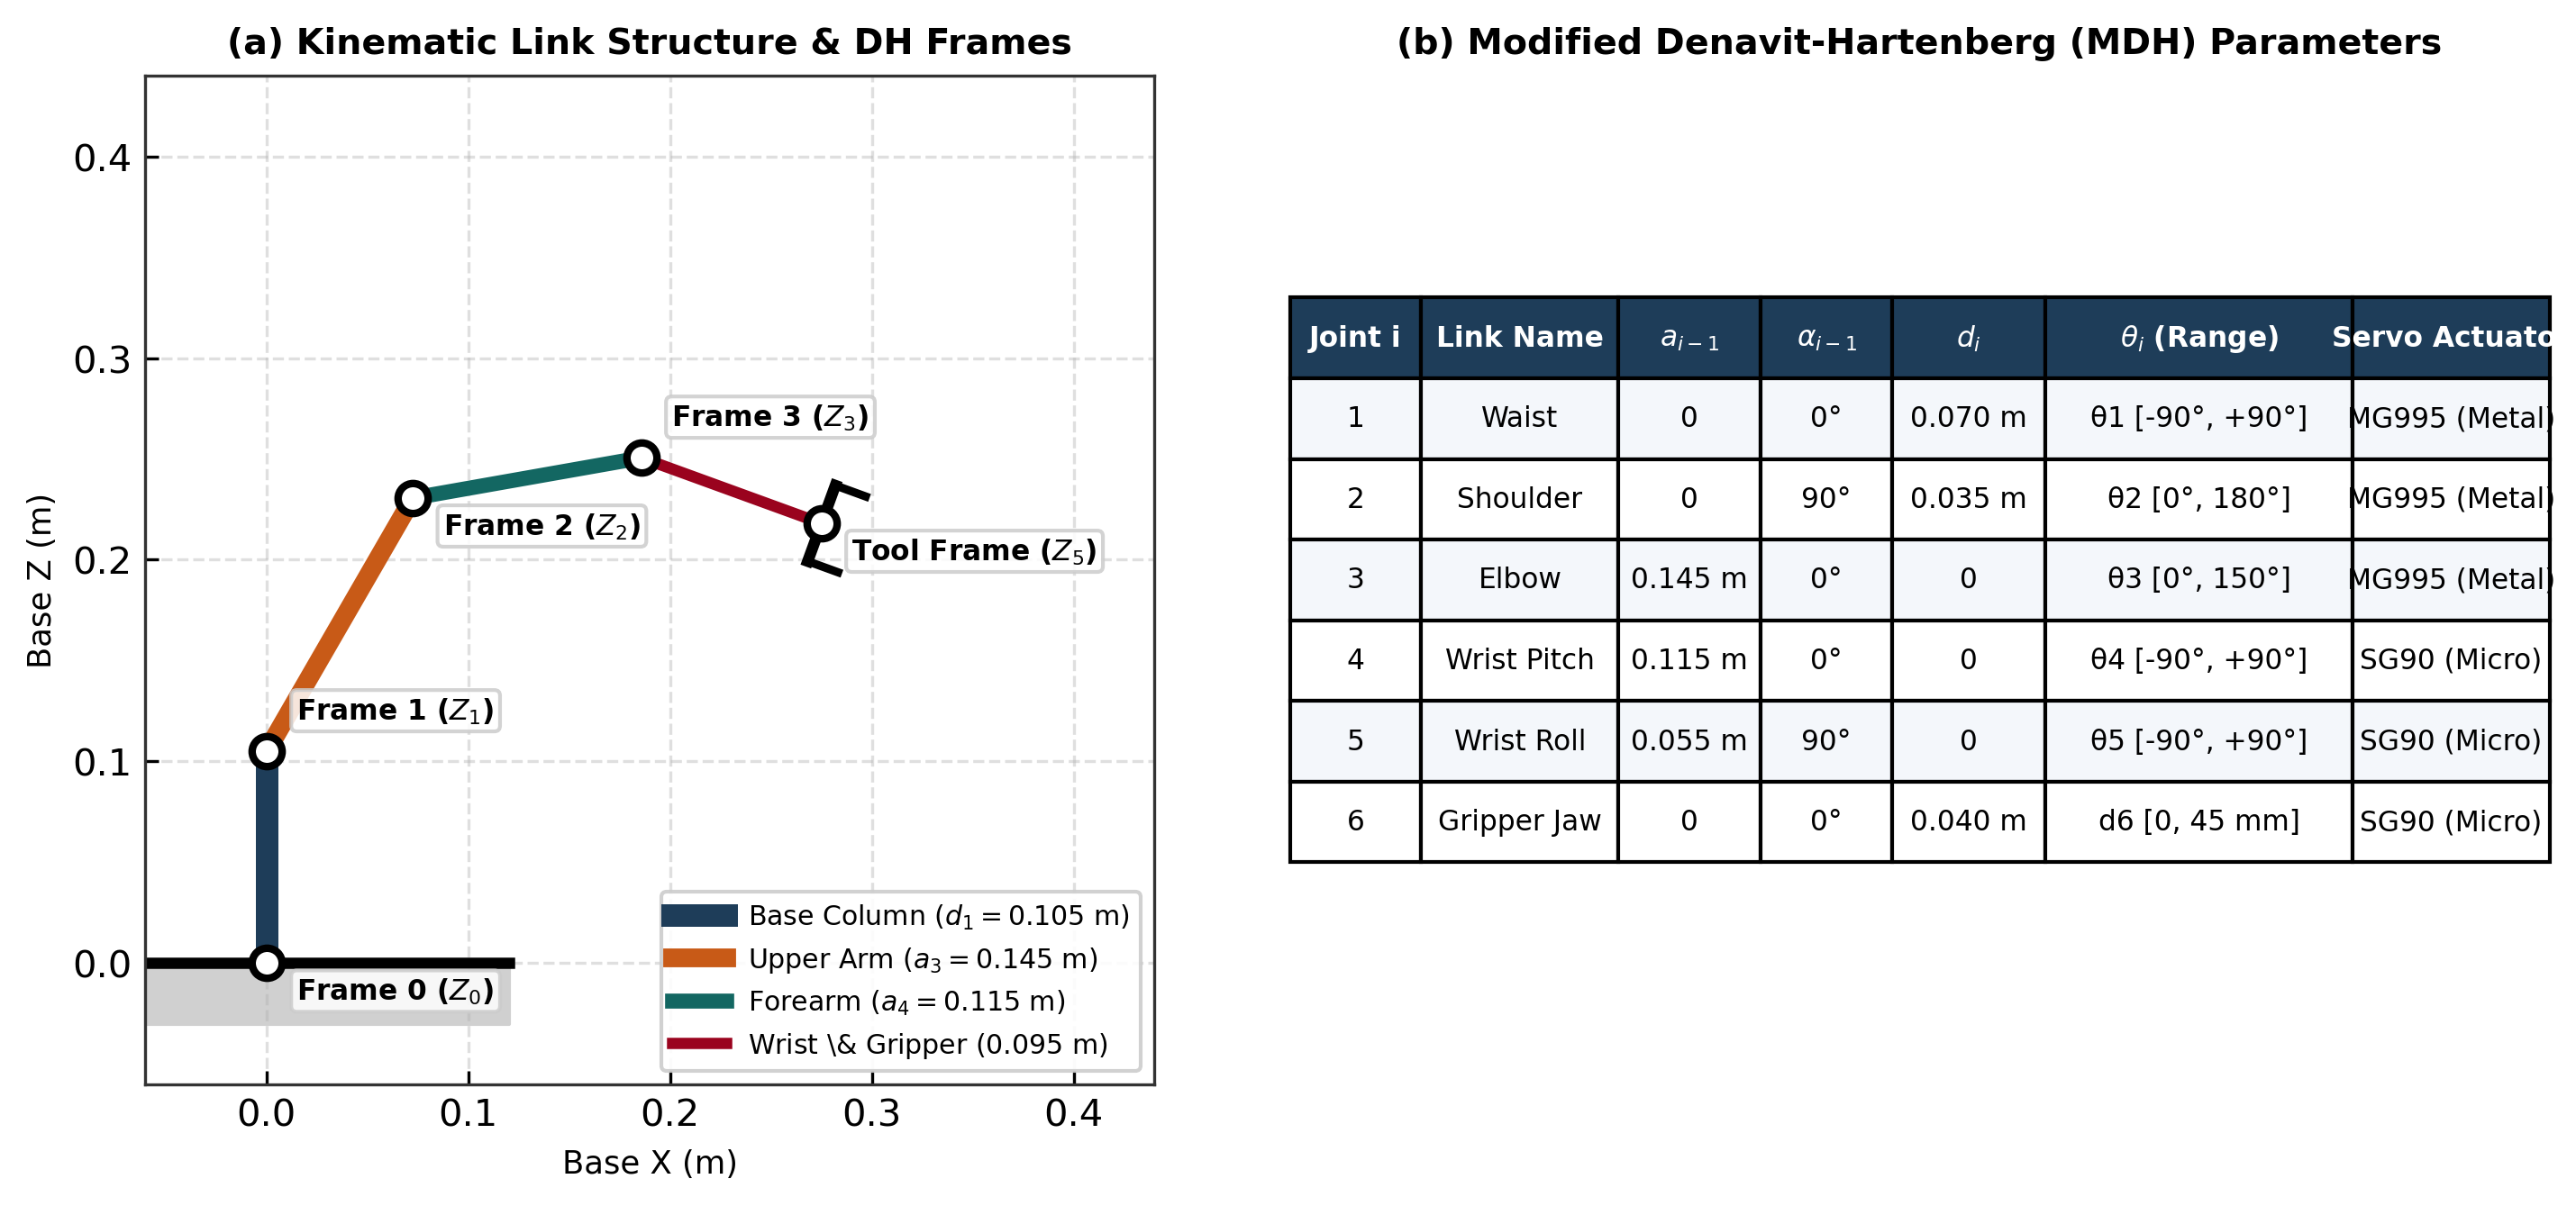
\includegraphics[width=\columnwidth]{fig2_kinematics_dh.png}
\caption{Kinematic chain and coordinate frame assignment for the 5-DoF ARIA manipulator following Modified Denavit-Hartenberg (Craig) conventions.}
\label{fig_kinematics_dh}
\end{figure}

\subsection{Modified Denavit-Hartenberg (Craig) Kinematic Formulation}
To establish the geometric relationship between adjacent articulated links, we adopt the Modified Denavit-Hartenberg (Craig) kinematic convention~\cite{aria_040_wagaa_2023_analytical}. In this convention, coordinate frame $\{i\}$ is rigidly attached to link $i$, with the $Z_i$ axis aligned with the axis of motion of joint $i+1$, and the $X_i$ axis directed along the common normal from $Z_i$ to $Z_{i+1}$. The four fundamental kinematic parameters are defined as:
\begin{itemize}
    \item $\alpha_{i-1}$: Link twist angle, representing the rotation from $Z_{i-1}$ to $Z_i$ about the common normal axis $X_{i-1}$.
    \item $a_{i-1}$: Link length, representing the distance from $Z_{i-1}$ to $Z_i$ measured along $X_{i-1}$.
    \item $d_i$: Link offset, representing the distance from $X_{i-1}$ to $X_i$ measured along the joint axis $Z_i$.
    \item $\theta_i$: Joint angle variable, representing the rotation from $X_{i-1}$ to $X_i$ about the joint axis $Z_i$.
\end{itemize}

The spatial frame assignments across all five revolute joints and the tool center point (TCP) are illustrated in Fig.~\ref{fig_kinematics_dh}. The precise numerical kinematic parameters, coordinate offsets, and dynamic operating bounds (expressed in the mathematical DH convention; see the note above Table~\ref{table_hardware_specs} for the mapping to raw servo coordinates) derived from the physical manipulator are cataloged in Table~\ref{table_dh_parameters}. Here, $a_2 = 0.145$\,m and $a_3 = 0.115$\,m specify the upper arm and forearm link lengths, while $d_5 = 0.095$\,m denotes the total tool offset from the wrist roll pivot to the fingertip plane ($L_{\text{wrist}} + L_{\text{grip}} = 0.055 + 0.040$\,m).

\begin{table}[!t]
\centering
\caption{Modified Denavit-Hartenberg (Craig) Parameters and Dynamic Operating Limits (Mathematical Joint Variables)}
\label{table_dh_parameters}
\footnotesize
\resizebox{\columnwidth}{!}{%
\begin{tabular}{ccccccc}
\toprule
\textbf{Link $i$} & \textbf{Joint Name} & \textbf{$\alpha_{i-1}$ (rad)} & \textbf{$a_{i-1}$ (m)} & \textbf{$d_i$ (m)} & \textbf{$\theta_i^{\text{DH}}$ Range (rad)} & \textbf{Max $\ddot{\theta}_i$ (rad/s$^2$)} \\
\midrule
1 & Waist & $0$ & $0$ & $d_1 = 0.105$ & $[-\pi/2, +\pi/2]$ & $15.0$ \\
2 & Shoulder & $+\frac{\pi}{2}$ & $a_1 = 0.030$ & $0$ & $[-\frac{\pi}{2}, +\frac{\pi}{2}]$ & $10.0$ \\
3 & Elbow & $0$ & $a_2 = 0.145$ & $0$ & $[-\frac{5\pi}{12}, +\frac{5\pi}{12}]$ & $12.0$ \\
4 & Wrist Pitch & $0$ & $a_3 = 0.115$ & $0$ & $[-\frac{\pi}{2}, +\frac{\pi}{2}]$ & $20.0$ \\
5 & Wrist Roll & $+\frac{\pi}{2}$ & $0$ & $d_5 = 0.095$ & $[-\frac{\pi}{2}, +\frac{\pi}{2}]$ & $25.0$ \\
\bottomrule
\end{tabular}%
}
\end{table}

Following Craig's convention, the general homogeneous transformation matrix relating coordinate frame $\{i-1\}$ to coordinate frame $\{i\}$ is parameterized by the product of fundamental screw motions:
\begin{equation}
\begin{split}
{}^{i-1}\mathbf{T}_i &= \text{Rot}_{X_{i-1}}(\alpha_{i-1}) \cdot \text{Trans}_{X_{i-1}}(a_{i-1}) \\
&\quad \cdot \text{Rot}_{Z_i}(\theta_i) \cdot \text{Trans}_{Z_i}(d_i)
\end{split}
\end{equation}
Evaluating the matrix multiplication yields the standard closed-form Craig transformation matrix:
\begin{equation}
{}^{i-1}\mathbf{T}_i = \left[\begin{array}{@{\hspace{2pt}}cccc@{\hspace{2pt}}}
c_i & -s_i & 0 & a_{i-1} \\
s_i c_{\alpha_{i-1}} & c_i c_{\alpha_{i-1}} & -s_{\alpha_{i-1}} & -d_i s_{\alpha_{i-1}} \\
s_i s_{\alpha_{i-1}} & c_i s_{\alpha_{i-1}} & c_{\alpha_{i-1}} & d_i c_{\alpha_{i-1}} \\
0 & 0 & 0 & 1
\end{array}\right]
\end{equation}
where $c_{\alpha_{i-1}} = \cos\alpha_{i-1}$ and $s_{\alpha_{i-1}} = \sin\alpha_{i-1}$.

Substituting the explicit DH parameters from Table~\ref{table_dh_parameters} into (2) for each link index yields the five elementary link transformation matrices:
{\setlength{\arraycolsep}{2pt}
\begin{align}
{}^0\mathbf{T}_1 &= \begin{bmatrix}
c_1 & -s_1 & 0 & 0 \\
s_1 & c_1 & 0 & 0 \\
0 & 0 & 1 & d_1 \\
0 & 0 & 0 & 1
\end{bmatrix}, \quad
{}^1\mathbf{T}_2 = \begin{bmatrix}
c_2 & -s_2 & 0 & a_1 \\
0 & 0 & -1 & 0 \\
s_2 & c_2 & 0 & 0 \\
0 & 0 & 0 & 1
\end{bmatrix} \\
{}^2\mathbf{T}_3 &= \begin{bmatrix}
c_3 & -s_3 & 0 & a_2 \\
s_3 & c_3 & 0 & 0 \\
0 & 0 & 1 & 0 \\
0 & 0 & 0 & 1
\end{bmatrix}, \quad
{}^3\mathbf{T}_4 = \begin{bmatrix}
c_4 & -s_4 & 0 & a_3 \\
s_4 & c_4 & 0 & 0 \\
0 & 0 & 1 & 0 \\
0 & 0 & 0 & 1
\end{bmatrix} \\
{}^4\mathbf{T}_5 &= \begin{bmatrix}
c_5 & -s_5 & 0 & 0 \\
0 & 0 & -1 & -d_5 \\
s_5 & c_5 & 0 & 0 \\
0 & 0 & 0 & 1
\end{bmatrix}
\end{align}
}
where we introduce the compact trigonometric shorthand $c_i = \cos\theta_i$, $s_i = \sin\theta_i$, $c_{ij} = \cos(\theta_i + \theta_j)$, $s_{ij} = \sin(\theta_i + \theta_j)$, $c_{ijk} = \cos(\theta_i + \theta_j + \theta_k)$, and $s_{ijk} = \sin(\theta_i + \theta_j + \theta_k)$.

\subsection{Symbolic Forward Kinematics Transformation}
The global forward kinematics map from the stationary manipulator base coordinate frame $\{0\}$ to the distal end-effector tool center point frame $\{5\}$ is synthesized via the consecutive post-multiplication of the individual link homogeneous transformation matrices:
\begin{equation}
{}^0\mathbf{T}_5(\boldsymbol{\theta}) = {}^0\mathbf{T}_1 \cdot {}^1\mathbf{T}_2 \cdot {}^2\mathbf{T}_3 \cdot {}^3\mathbf{T}_4 \cdot {}^4\mathbf{T}_5 = \begin{bmatrix}
\mathbf{n} & \mathbf{s} & \mathbf{a} & \mathbf{P} \\
0 & 0 & 0 & 1
\end{bmatrix}
\end{equation}
where $\mathbf{n} = [n_x, n_y, n_z]^T$, $\mathbf{s} = [s_x, s_y, s_z]^T$, and $\mathbf{a} = [a_x, a_y, a_z]^T$ designate the orthogonal normal, sliding, and approach unit vectors defining the end-effector orientation matrix $\mathbf{R} \in SO(3)$, and $\mathbf{P} = [P_x, P_y, P_z]^T$ represents the Cartesian coordinates of the tool center point in base frame $\{0\}$.

Performing symbolic matrix reduction yields the explicit algebraic equations governing Cartesian tool center point positioning:
\begin{align}
P_x &= c_1 \left( a_1 + a_2 c_2 + a_3 c_{23} + d_5 c_{234} \right) \\
P_y &= s_1 \left( a_1 + a_2 c_2 + a_3 c_{23} + d_5 c_{234} \right) \\
P_z &= d_1 + a_2 s_2 + a_3 s_{23} + d_5 s_{234}
\end{align}
Similarly, the components of the end-effector tool orientation rotation matrix $\mathbf{R} = [\mathbf{n}, \mathbf{s}, \mathbf{a}]$ are given by:
\begin{equation}
\mathbf{R} = \begin{bmatrix}
c_1 c_{234} c_5 - s_1 s_5 & -c_1 c_{234} s_5 - s_1 c_5 & c_1 s_{234} \\
s_1 c_{234} c_5 + c_1 s_5 & -s_1 c_{234} s_5 + c_1 c_5 & s_1 s_{234} \\
s_{234} c_5 & -s_{234} s_5 & -c_{234}
\end{bmatrix}
\end{equation}

\begin{assumption}[Manipulator Kinematic Rigidity and Actuation Envelopes]
\label{ass_rigidity}
The 5-DoF anthropomorphic manipulator is modeled as an open serial kinematic chain comprising five rigid links interconnected by revolute joints with invariant link lengths $a_i$ and offsets $d_i$. The joint displacements $\boldsymbol{\theta} \in \mathbb{R}^5$ are constrained within compact mechanical operating envelopes $\boldsymbol{\theta}_{\min} \le \boldsymbol{\theta} \le \boldsymbol{\theta}_{\max}$, and angular velocities satisfy $|\dot{\theta}_i| \le \dot{\theta}_{i,\max}$ enforced by closed-loop potentiometer telemetry.
\end{assumption}

Because the manipulator has five actuated degrees of freedom, it cannot in general realize an arbitrary target in $SE(3)$, which has six independent pose coordinates. We therefore restrict attention to the manipulator's \emph{admissible task manifold}, in which end-effector position is fully specified and orientation is parameterized by a single independent pitch/roll pair consistent with the geometric coupling of the chain (Section~III-D):
\begin{equation}
\mathcal{M}_{\text{task}} = \left\{ (\mathbf{P}, \phi, \psi) \in \mathbb{R}^3 \times \mathbb{R} \times \mathbb{R} : \mathbf{P}\in\mathcal{W} \right\} \subset SE(3),
\end{equation}
where $\phi$ is the commanded global end-effector pitch (Section~III-D-4) and $\psi$ is the commanded wrist roll (Section~III-D-5), and $\mathcal{W}\subset\mathbb{R}^3$ is the reachable positional workspace. $\mathcal{M}_{\text{task}}$ is a 5-dimensional admissible subset of $SE(3)$, consistent with the manipulator's 5 actuated joints.

\begin{proposition}[Closed-Form Inverse Kinematics on the Admissible Task Manifold]
\label{prop_ik}
For any target pose $(\mathbf{P}_{\text{target}}, \phi_{\text{target}}, \psi_{\text{target}}) \in \mathcal{M}_{\text{task}}$ satisfying the reachability condition of (18) and the joint limits of Assumption~\ref{ass_rigidity}, the geometric decoupling of the anthropomorphic chain (Section~III-D) yields a finite set of analytical joint configurations $\boldsymbol{\theta}^* = [\theta_1^*, \theta_2^*, \theta_3^*, \theta_4^*, \theta_5^*]^T$ (one elbow-up and one elbow-down branch, of which ARIA deterministically selects the elbow-up branch), computable in closed form without iterative search, in a mean measured solve time of $0.08$\,ms on the reference host (Section~IX-A). The procedure explicitly flags targets outside $\mathcal{W}$ or outside the joint limits as unreachable, and explicitly flags the three singularity regimes of Section~III-F, rather than silently returning a degraded solution. For targets outside $\mathcal{M}_{\text{task}}$ (i.e., orientation requests inconsistent with the coupling in (21)), no exact solution exists and the solver returns an infeasibility flag.
\end{proposition}

\subsection{Exact Closed-Form Analytical Inverse Kinematics Derivation}
Given a desired end-effector target pose on the admissible task manifold $\mathcal{M}_{\text{task}}$, defined by target Cartesian position $\mathbf{P}_{\text{target}} = [P_x, P_y, P_z]^T$ and target approach direction $\mathbf{a} = [a_x, a_y, a_z]^T$ consistent with commanded pitch $\phi_{\text{target}}$, the objective of the inverse kinematics routine is to compute the joint-space vector $\boldsymbol{\theta} = [\theta_1, \theta_2, \theta_3, \theta_4, \theta_5]^T$ that satisfies the forward kinematics identity $\mathbf{T}_5^0(\boldsymbol{\theta}) = \mathbf{T}_{\text{target}}$.

While general-purpose robotics frameworks (e.g., KDL, TRAC-IK, IKPy, cuRobo~\cite{aria_050_sundaralingam_2024_curobo}, and high-stiffness planners~\cite{aria_044_pang_2025_highstiffness}) formulate inverse kinematics as a nonlinear optimization problem solved via iterative numerical Jacobian inversion, such routines carry per-solve computational cost and can occasionally fail to converge on 5-DoF chains. As established above, the end-effector orientation cannot be specified fully independently of arm position on this manipulator ($m=5<6$). We therefore derive a closed-form solution restricted to $\mathcal{M}_{\text{task}}$ by decomposing the chain into decoupled geometric subproblems.

\subsubsection{Subproblem 1: Base Azimuth Angle ($\theta_1$)}
Inspecting the position equations (7) and (8), we observe that the term within brackets, $R_{\text{arm}} = a_1 + a_2 c_2 + a_3 c_{23} + d_5 c_{234}$, is identical in both $P_x$ and $P_y$. Dividing (8) by (7) eliminates the four-joint planar linkage terms:
\begin{equation}
\frac{P_y}{P_x} = \frac{s_1 R_{\text{arm}}}{c_1 R_{\text{arm}}} = \frac{s_1}{c_1} = \tan\theta_1
\end{equation}
Applying the four-quadrant arctangent function yields the closed-form solution for the base azimuth angle:
\begin{equation}
\theta_1 = \text{atan2}(P_y, P_x)
\end{equation}
\textit{Singularity Handling}: In the configuration where $P_x = 0$ and $P_y = 0$, the tool center point lies on the vertical $Z_0$ base axis and $\theta_1$ is mathematically indeterminate. ARIA flags this shoulder-axis singularity condition (Section~III-F) and, to avoid high-velocity motor chatter, holds the previous joint setpoint $\theta_1^{(k)} = \theta_1^{(k-1)}$ while the flag is active.

\subsubsection{Subproblem 2: Wrist Center Decoupling}
With $\theta_1$ established, we decouple the orientation of the distal wrist and gripper from the planar two-link arm mechanism. The Cartesian position of the wrist pitch axis center, $\mathbf{P}_w = [P_{wx}, P_{wy}, P_{wz}]^T$, is obtained by translating backwards from the desired tool center point $\mathbf{P}$ along the tool approach vector $\mathbf{a}$ by tool offset $d_5$:
\begin{equation}
\mathbf{P}_w = \mathbf{P} - d_5 \mathbf{a} = \begin{bmatrix}
P_x - d_5 a_x \\
P_y - d_5 a_y \\
P_z - d_5 a_z
\end{bmatrix}
\end{equation}

\subsubsection{Subproblem 3: Planar 2R Arm Geometry ($\theta_2, \theta_3$)}
The physical coordinates of the wrist center $\mathbf{P}_w$ project onto the planar 2R sagittal plane of the shoulder and elbow joints. We compute the planar horizontal reach radius $r$ and vertical elevation $s$ relative to the shoulder joint origin $\{2\}$:
\begin{align}
r &= \sqrt{P_{wx}^2 + P_{wy}^2} - a_1 \\
s &= P_{wz} - d_1
\end{align}
The Euclidean distance squared from the shoulder joint axis $\{2\}$ to the wrist center $\{4\}$ satisfies the geometric constraint:
\begin{equation}
D^2 = r^2 + s^2 = a_2^2 + a_3^2 + 2 a_2 a_3 \cos\theta_3
\end{equation}
Rearranging (16) via the algebraic Law of Cosines yields the exact expression for the cosine of the elbow joint angle:
\begin{equation}
\cos\theta_3 = \frac{r^2 + s^2 - a_2^2 - a_3^2}{2 a_2 a_3}
\end{equation}

\textit{Reachability Condition}: A valid kinematic solution on $\mathcal{M}_{\text{task}}$ exists if and only if:
\begin{equation}
-1.0 \le \frac{r^2 + s^2 - a_2^2 - a_3^2}{2 a_2 a_3} \le +1.0
\end{equation}
If $|\cos\theta_3| > 1.0$, the commanded Cartesian coordinate lies strictly outside the workspace $\mathcal{W}$. In this case the solver returns an out-of-reach flag without invoking numerical optimization. For all reachable poses satisfying (18), two symmetric kinematic branches exist: elbow-up ($\theta_3 < 0$) and elbow-down ($\theta_3 > 0$). To maximize mechanical ground clearance and avoid workspace tabletop collisions, ARIA deterministically selects the elbow-up branch:
\begin{equation}
\theta_3 = -\arccos\left( \frac{r^2 + s^2 - a_2^2 - a_3^2}{2 a_2 a_3} \right)
\end{equation}

With $\theta_3$ resolved, we compute the shoulder pitch angle $\theta_2$ by decomposing the planar elevation angle into the sum of two trigonometric angles:
\begin{equation}
\theta_2 = \text{atan2}(s, r) - \text{atan2}\left(a_3 \sin\theta_3, \, a_2 + a_3 \cos\theta_3\right)
\end{equation}

\subsubsection{Subproblem 4: Wrist Pitch Angle ($\theta_4$)}
In anthropomorphic articulated arms with parallel horizontal pitch axes ($Z_2 \parallel Z_3 \parallel Z_4$), the global pitch angle of the end-effector relative to the horizontal ground plane is the cumulative sum of the sagittal joint angles:
\begin{equation}
\phi_{\text{pitch}} = \theta_2 + \theta_3 + \theta_4
\end{equation}
This relation is the geometric coupling that restricts admissible orientations to $\mathcal{M}_{\text{task}}$: once $\theta_2,\theta_3$ are fixed by the position solution, only a one-parameter family of global pitch angles $\phi_{\text{target}}$ remains freely assignable via $\theta_4$, within its joint limit. Depending on the task requirements (e.g., $\phi_{\text{target}} = -\frac{\pi}{2}$ for top-down pick-and-place, or $\phi_{\text{target}} = 0$ for horizontal conveyor side-approach), the wrist pitch joint setpoint is computed as:
\begin{equation}
\theta_4 = \phi_{\text{target}} - (\theta_2 + \theta_3)
\end{equation}
If the resulting $\theta_4$ violates its joint limit, the target lies outside $\mathcal{M}_{\text{task}}$ and the solver returns an orientation-infeasibility flag.

\subsubsection{Subproblem 5: Wrist Roll Angle ($\theta_5$)}
Finally, to align the gripper jaws with the workpiece orientation $\psi_{\text{target}}$ relative to the workspace coordinate frame, the wrist roll joint $\theta_5$ rotates the claw about the tool approach vector:
\begin{equation}
\theta_5 = \psi_{\text{target}} - \theta_1
\end{equation}
If no specific workpiece roll angle is commanded, $\theta_5$ is held at $0.0$\,rad to maintain a neutral vertical claw orientation.

The complete deterministic closed-form inverse kinematics procedure, including boundary condition checking and hardware limit clamping, is formalized in Algorithm~\ref{alg_analytical_ik}.

\begin{algorithm}[!t]
\caption{ARIA Closed-Form Analytical 5-DoF Inverse Kinematics Solver on $\mathcal{M}_{\text{task}}$}
\label{alg_analytical_ik}
\begin{algorithmic}[1]
\REQUIRE Target TCP pose $\mathbf{P} = [P_x, P_y, P_z]^T$, pitch angle $\phi_{\text{target}}$, yaw angle $\psi_{\text{target}}$, previous joint state $\boldsymbol{\theta}_{\text{prev}}$
\ENSURE Valid joint setpoints $\boldsymbol{\theta}^* = [\theta_1^*, \theta_2^*, \theta_3^*, \theta_4^*, \theta_5^*]^T$, or Reachability/Orientation-Infeasibility Error Flag
\STATE \textbf{// Step 1: Base Azimuth Angle ($\theta_1$)}
\IF{$|P_x| < 10^{-4}$ \AND $|P_y| < 10^{-4}$}
    \STATE $\theta_1 \leftarrow \theta_{1, \text{prev}}$ \COMMENT{Flag shoulder-axis singularity; hold last setpoint}
\ELSE
    \STATE $\theta_1 \leftarrow \text{atan2}(P_y, P_x)$
\ENDIF
\STATE \textbf{// Step 2: Wrist Center Decoupling}
\STATE $a_x \leftarrow \cos\theta_1 \cos\phi_{\text{target}}$, $a_y \leftarrow \sin\theta_1 \cos\phi_{\text{target}}$, $a_z \leftarrow \sin\phi_{\text{target}}$
\STATE $P_{wx} \leftarrow P_x - d_5 a_x$, $P_{wy} \leftarrow P_y - d_5 a_y$, $P_{wz} \leftarrow P_z - d_5 a_z$
\STATE \textbf{// Step 3: Planar 2R Linkage Geometry}
\STATE $r \leftarrow \sqrt{P_{wx}^2 + P_{wy}^2} - a_1$, $s \leftarrow P_{wz} - d_1$
\STATE $C_3 \leftarrow \frac{r^2 + s^2 - a_2^2 - a_3^2}{2 a_2 a_3}$
\IF{$C_3 < -1.0$ \OR $C_3 > 1.0$}
    \RETURN \textbf{ERROR: Target Outside Reachable Workspace $\mathcal{W}$}
\ENDIF
\STATE $\theta_3 \leftarrow -\arccos(C_3)$ \COMMENT{Elbow-Up Branch}
\STATE $\theta_2 \leftarrow \text{atan2}(s, r) - \text{atan2}(a_3 \sin\theta_3, a_2 + a_3 C_3)$
\STATE \textbf{// Step 4: Wrist Pitch \& Roll Angles}
\STATE $\theta_4 \leftarrow \phi_{\text{target}} - (\theta_2 + \theta_3)$
\STATE $\theta_5 \leftarrow \psi_{\text{target}} - \theta_1$
\STATE \textbf{// Step 5: Hardware Joint Limit Verification}
\FOR{$i = 1$ \TO $5$}
    \IF{$\theta_i < \theta_{i, \text{min}}$ \OR $\theta_i > \theta_{i, \text{max}}$}
        \RETURN \textbf{ERROR: Joint Limit Exceeded at Joint $i$ (target outside $\mathcal{M}_{\text{task}}$)}
    \ENDIF
\ENDFOR
\RETURN $\boldsymbol{\theta}^* = [\theta_1, \theta_2, \theta_3, \theta_4, \theta_5]^T$
\end{algorithmic}
\end{algorithm}

\subsection{Differential Kinematics \& Geometric Jacobian Derivation}
The mapping between joint velocity vector $\dot{\boldsymbol{\theta}} = [\dot{\theta}_1, \dot{\theta}_2, \dot{\theta}_3, \dot{\theta}_4, \dot{\theta}_5]^T$ and Cartesian linear/angular velocity of the tool center point $\mathbf{v} = [\mathbf{v}_p^T, \boldsymbol{\omega}^T]^T \in \mathbb{R}^6$ is governed by the geometric Jacobian matrix $\mathbf{J}(\boldsymbol{\theta}) \in \mathbb{R}^{6\times5}$:
\begin{equation}
\begin{bmatrix} \mathbf{v}_p \\ \boldsymbol{\omega} \end{bmatrix} = \mathbf{J}(\boldsymbol{\theta}) \dot{\boldsymbol{\theta}} = \begin{bmatrix} \mathbf{J}_v(\boldsymbol{\theta}) \\ \mathbf{J}_\omega(\boldsymbol{\theta}) \end{bmatrix} \dot{\boldsymbol{\theta}}
\end{equation}
For an articulated chain comprising revolute joints, the $i$-th column of the geometric Jacobian is formulated as:
\begin{equation}
\mathbf{J}_i(\boldsymbol{\theta}) = \begin{bmatrix} \mathbf{J}_{v, i} \\ \mathbf{J}_{\omega, i} \end{bmatrix} = \begin{bmatrix} \mathbf{z}_{i-1} \times (\mathbf{P} - \mathbf{p}_{i-1}) \\ \mathbf{z}_{i-1} \end{bmatrix}
\end{equation}
where $\mathbf{z}_{i-1}$ denotes the unit vector along joint axis $i$, $\mathbf{p}_{i-1}$ represents the origin of coordinate frame $\{i-1\}$, and $\mathbf{P}$ is the tool center point position, all expressed in base frame $\{0\}$.

Evaluating (25) using the link transformation matrices (3)–(5) yields the explicit columns of the ARIA geometric Jacobian:
\begin{align}
\mathbf{J}_1 &= \begin{bmatrix} -P_y \\ P_x \\ 0 \\ 0 \\ 0 \\ 1 \end{bmatrix}, \quad
\mathbf{J}_2 = \begin{bmatrix} -s_1 (P_z - d_1) \\ c_1 (P_z - d_1) \\ -c_1 (P_x - a_1 c_1) - s_1 (P_y - a_1 s_1) \\ -s_1 \\ c_1 \\ 0 \end{bmatrix} \\
\mathbf{J}_3 &= \begin{bmatrix} -s_1 (P_z - d_1 - a_2 s_2) \\ c_1 (P_z - d_1 - a_2 s_2) \\ -c_1 (P_x - c_1(a_1 + a_2 c_2)) - s_1 (P_y - s_1(a_1 + a_2 c_2)) \\ -s_1 \\ c_1 \\ 0 \end{bmatrix} \\
\mathbf{J}_4 &= \begin{bmatrix} -s_1 d_5 s_{234} \\ c_1 d_5 s_{234} \\ -c_1 d_5 c_{234} \\ -s_1 \\ c_1 \\ 0 \end{bmatrix}, \quad
\mathbf{J}_5 = \begin{bmatrix} 0 \\ 0 \\ 0 \\ c_1 s_{234} \\ s_1 s_{234} \\ -c_{234} \end{bmatrix}
\end{align}
Since $\mathbf{J}(\boldsymbol{\theta}) \in \mathbb{R}^{6\times5}$ has at most 5 linearly independent rows, it is not square and its row space cannot span all of $\mathbb{R}^6$; one instantaneous Cartesian direction (the orientation degree of freedom not independently actuated) is always unrealizable, consistent with $\mathcal{M}_{\text{task}}$ above.

\subsection{Kinematic Singularity \& Manipulability Analysis}
Kinematic singularities represent configurations in which the geometric Jacobian matrix experiences rank deficiency ($\text{rank}(\mathbf{J}) < 5$), resulting in the loss of one or more instantaneous operational degrees of freedom \emph{within the 5-dimensional controlled subspace}. Because $\mathbf{J}\in\mathbb{R}^{6\times5}$ is not square, the product $\mathbf{J}\mathbf{J}^T\in\mathbb{R}^{6\times6}$ is rank-deficient by construction (rank $\le 5 < 6$) and is singular \emph{everywhere}, so $\det(\mathbf{J}\mathbf{J}^T) \equiv 0$ regardless of configuration; the classical Yoshikawa measure $w=\sqrt{\det(\mathbf{J}\mathbf{J}^T)}$ is therefore not an applicable manipulability index for this Jacobian shape and we do not use it. Instead, we quantify dexterity over the controlled 5-dimensional subspace using the reduced Gram determinant
\begin{equation}
w_5(\boldsymbol{\theta}) = \sqrt{\det\left( \mathbf{J}^T(\boldsymbol{\theta})\, \mathbf{J}(\boldsymbol{\theta}) \right)},
\end{equation}
where $\mathbf{J}^T\mathbf{J}\in\mathbb{R}^{5\times5}$; equivalently $w_5(\boldsymbol{\theta}) = \prod_{k=1}^{5}\sigma_k(\mathbf{J})$, the product of the (up to) five nonzero singular values of $\mathbf{J}$. As with the classical measure, $w_5(\boldsymbol{\theta})\to 0$ as the arm approaches a configuration in which $\mathbf{J}$ loses column rank, indicating that some joint-velocity combination produces vanishing Cartesian motion.

Through inspection of the Jacobian columns (26)–(28), we identify three configurations at which $\mathbf{J}$ loses column rank on the ARIA platform:
\begin{enumerate}
    \item \textbf{Boundary Reach Singularities}: Occur when the arm is fully outstretched ($r^2 + s^2 = (a_2 + a_3)^2 \implies \theta_3 = 0.0$\,rad) or completely folded back onto itself ($r^2 + s^2 = (a_2 - a_3)^2 \implies \theta_3 = \pi$\,rad). In this state, $\sin\theta_3 = 0$, eliminating instantaneous radial velocity along the arm's longitudinal direction.
    \item \textbf{Shoulder Axis Singularities}: Occur when the wrist center axis intersects the vertical base rotation axis $Z_0$ ($r = 0$). In this configuration, azimuth rotation $\dot{\theta}_1$ produces zero linear motion, causing base yaw velocity to become redundant.
    \item \textbf{Pitch Alignment Singularities}: Occur when the end-effector approach axis aligns collinear with the forearm link vector ($\theta_4 = 0.0$\,rad with $s_{234} = 0$), causing wrist pitch and shoulder pitch motions to project onto degenerate instantaneous velocity subspaces.
\end{enumerate}

Because the ARIA analytical inverse kinematics algorithm directly solves the geometric equations (11)–(23) rather than computing a Jacobian pseudo-inverse (for a full-column-rank $\mathbf{J}$, the left pseudo-inverse $\mathbf{J}^{\dagger} = (\mathbf{J}^T\mathbf{J})^{-1}\mathbf{J}^T$; a damped least-squares variant $\mathbf{J}^{\dagger}_{\lambda} = (\mathbf{J}^T\mathbf{J} + \lambda^2\mathbf{I})^{-1}\mathbf{J}^T$ is typically used near rank deficiency), it avoids the numerical ill-conditioning associated with inverting a near-singular Gram matrix. This distinction is one of \emph{numerical conditioning}, not of physical singularity avoidance: the analytical solver explicitly detects and flags the three singularity regimes above (via $C_3\to\pm1$, $r\to0$, and $s_{234}\to0$ respectively) rather than eliminating them, and we revise our terminology accordingly: the solver avoids \emph{iterative numerical non-convergence}, not the underlying kinematic singularities themselves.

\subsection{Euler-Lagrange Dynamic Modeling \& Gravity Compensation}
Accurate physical simulation within the Gazebo digital twin and feedforward trajectory control on the physical arm require the explicit formulation of the manipulator equations of motion. Following the Euler-Lagrange formalization, the continuous dynamic model of the 5-DoF articulated arm is expressed in standard matrix form:
\begin{equation}
\mathbf{M}(\mathbf{q})\ddot{\mathbf{q}} + \mathbf{C}(\mathbf{q}, \dot{\mathbf{q}})\dot{\mathbf{q}} + \mathbf{G}(\mathbf{q}) + \mathbf{F}_v \dot{\mathbf{q}} + \mathbf{F}_s \text{sgn}(\dot{\mathbf{q}}) = \boldsymbol{\tau}
\end{equation}
where $\mathbf{q} \in \mathbb{R}^5$ is the vector of generalized joint coordinates ($\mathbf{q} \equiv \boldsymbol{\theta}$), $\mathbf{M}(\mathbf{q}) \in \mathbb{R}^{5\times5}$ is the symmetric, positive-definite generalized mass/inertia matrix, $\mathbf{C}(\mathbf{q}, \dot{\mathbf{q}}) \in \mathbb{R}^{5\times5}$ represents Coriolis and centrifugal dynamic effects, $\mathbf{G}(\mathbf{q}) \in \mathbb{R}^5$ is the gravitational torque vector, $\mathbf{F}_v, \mathbf{F}_s \in \mathbb{R}^{5\times5}$ denote diagonal viscous and Coulomb friction coefficients, and $\boldsymbol{\tau} \in \mathbb{R}^5$ represents the vector of generalized actuator torques. This model is used only for Gazebo simulation tuning and open-loop feedforward gravity compensation; joint torques are not directly measured on the physical platform, and $\mathbf{F}_v,\mathbf{F}_s$ are approximate, identified offline.

The kinetic energy $K(\mathbf{q}, \dot{\mathbf{q}})$ of the manipulator is the sum of translational and rotational kinetic energies across all articulated links:
\begin{equation}
K(\mathbf{q}, \dot{\mathbf{q}}) = \frac{1}{2} \sum_{i=1}^5 \left( m_i \mathbf{v}_{c_i}^T \mathbf{v}_{c_i} + \boldsymbol{\omega}_i^T \mathbf{I}_i \boldsymbol{\omega}_i \right) = \frac{1}{2} \dot{\mathbf{q}}^T \mathbf{M}(\mathbf{q}) \dot{\mathbf{q}}
\end{equation}
where $m_i$ is the mass of link $i$, $\mathbf{v}_{c_i}$ is the linear velocity of the link center of mass, $\boldsymbol{\omega}_i$ is the link angular velocity, and $\mathbf{I}_i$ is the $3\times3$ centroidal inertia tensor of link $i$.

The gravitational potential energy $P(\mathbf{q})$ is defined with respect to the horizontal tabletop reference datum:
\begin{equation}
P(\mathbf{q}) = \sum_{i=1}^5 m_i \mathbf{g}^T \mathbf{p}_{c_i}(\mathbf{q})
\end{equation}
where $\mathbf{g} = [0, 0, -9.81]^T$\,m/s$^2$ is the gravity vector, and $\mathbf{p}_{c_i}(\mathbf{q})$ represents the Cartesian position of the center of mass of link $i$.

The elements of the Coriolis and centrifugal matrix $\mathbf{C}(\mathbf{q}, \dot{\mathbf{q}})$ are derived from the mass matrix $\mathbf{M}(\mathbf{q})$ via the Christoffel symbols of the first kind:
\begin{equation}
c_{ij} = \sum_{k=1}^5 c_{ijk} \dot{q}_k = \frac{1}{2} \sum_{k=1}^5 \left( \frac{\partial m_{ij}}{\partial q_k} + \frac{\partial m_{ik}}{\partial q_j} - \frac{\partial m_{jk}}{\partial q_i} \right) \dot{q}_k
\end{equation}
The gravity compensation vector $\mathbf{G}(\mathbf{q})$ is obtained directly from the partial derivatives of the potential energy:
\begin{equation}
G_i(\mathbf{q}) = \frac{\partial P(\mathbf{q})}{\partial q_i}
\end{equation}

For the ARIA 5-DoF manipulator, the explicit gravity compensation torques for the dominant sagittal pitch joints (Joints 2, 3, and 4) are evaluated as:
\begin{align}
G_1(\mathbf{q}) &= 0 \\
G_2(\mathbf{q}) &= g \left( m_2 r_{c2} c_2 + m_3 (a_2 c_2 + r_{c3} c_{23}) \right. \nonumber \\
                &\quad \left. + (m_4 + m_5 + m_{\text{load}}) (a_2 c_2 + a_3 c_{23} + r_{c4} c_{234}) \right) \\
G_3(\mathbf{q}) &= g m_3 r_{c3} c_{23} \nonumber \\
                &\quad + g (m_4 + m_5 + m_{\text{load}}) (a_3 c_{23} + r_{c4} c_{234}) \\
G_4(\mathbf{q}) &= g (m_4 + m_5 + m_{\text{load}}) r_{c4} c_{234} \\
G_5(\mathbf{q}) &= 0
\end{align}
where $r_{ci}$ denotes the radial distance from joint axis $i$ to the center of mass of link $i$. The physical mass distribution and inertial properties parameterized in the Gazebo URDF model are documented in Table~\ref{table_dynamics_params}.

\begin{table}[!t]
\centering
\caption{Mass Distribution and Principal Inertia Parameters for Dynamic Modeling}
\label{table_dynamics_params}
\footnotesize
\resizebox{\columnwidth}{!}{%
\begin{tabular}{lccccc}
\toprule
\textbf{Link $i$} & \textbf{Mass $m_i$ (kg)} & \textbf{CoM $r_{ci}$ (m)} & \textbf{$I_{xx}$ (kg$\cdot$m$^2$)} & \textbf{$I_{yy}$ (kg$\cdot$m$^2$)} & \textbf{$I_{zz}$ (kg$\cdot$m$^2$)} \\
\midrule
Link 1 (Base) & $0.185$ & $[0, 0, 0.052]$ & $1.82 \times 10^{-4}$ & $1.82 \times 10^{-4}$ & $2.14 \times 10^{-4}$ \\
Link 2 (Upper Arm) & $0.240$ & $[0.072, 0, 0.015]$ & $3.45 \times 10^{-4}$ & $8.92 \times 10^{-4}$ & $8.15 \times 10^{-4}$ \\
Link 3 (Forearm) & $0.165$ & $[0.068, 0, 0.010]$ & $1.95 \times 10^{-4}$ & $5.21 \times 10^{-4}$ & $4.85 \times 10^{-4}$ \\
Link 4 (Wrist Pitch) & $0.065$ & $[0.025, 0, 0]$ & $4.20 \times 10^{-5}$ & $6.15 \times 10^{-5}$ & $5.80 \times 10^{-5}$ \\
Link 5 (End-Effector) & $0.085$ & $[0.035, 0, 0]$ & $5.10 \times 10^{-5}$ & $7.40 \times 10^{-5}$ & $6.90 \times 10^{-5}$ \\
\bottomrule
\end{tabular}%
}
\end{table}

% ====================================================================
% SECTION IV: MULTI-AGENT ARCHITECTURE
% ====================================================================
\section{Modular Asynchronous Multi-Agent System Architecture}

\subsection{Architectural Paradigm \& State Bus}
Traditional robotic control frameworks (such as early ROS 1 implementations or monolithic robotic foundation models) structure software around either tightly coupled synchronous execution loops or a single end-to-end neural network. In monolithic foundation approaches (e.g., OpenVLA, Octo), a deep transformer processes pixel arrays and language tokens to output joint setpoints. This formulation carries some structural risks: a perceptual anomaly can propagate directly into motor output, intermediate reasoning is not exposed for inspection, and reported inference latencies ($>85$\,ms in the policies benchmarked in Section~IX-B) can affect closed-loop responsiveness.

To pursue an alternative design point, Project ARIA introduces a \textbf{modular, asynchronous, service-oriented software architecture} grounded in the Robot Operating System 2 (ROS 2) Humble middleware. As illustrated in Fig.~\ref{fig_system_architecture}, the system is organized into six functional tiers comprising fifteen software modules -- which we refer to as \emph{agents} in the specific, scoped sense defined below -- each implemented as an independently lifecycle-managed ROS~2 node communicating asynchronously over a shared \textbf{State Bus}. We use the term \emph{agent} to denote a module that (i) maintains locally encapsulated state, (ii) is independently configurable, activatable, and recoverable through the ROS~2 managed-lifecycle interface (Section~IV-C), and (iii) communicates with other modules only through asynchronous State Bus messages rather than direct function calls; we do not claim inter-agent negotiation, learning, or autonomy beyond this scoped definition. All fifteen agents currently execute as separate processes on a single host and communicate over local ROS~2 DDS topics; the architecture is therefore more accurately described as \emph{modular and asynchronous} than as \emph{distributed} in the distributed-systems sense, since we have not evaluated deployment across physically separate hosts.

\begin{figure*}[!t]
\centering
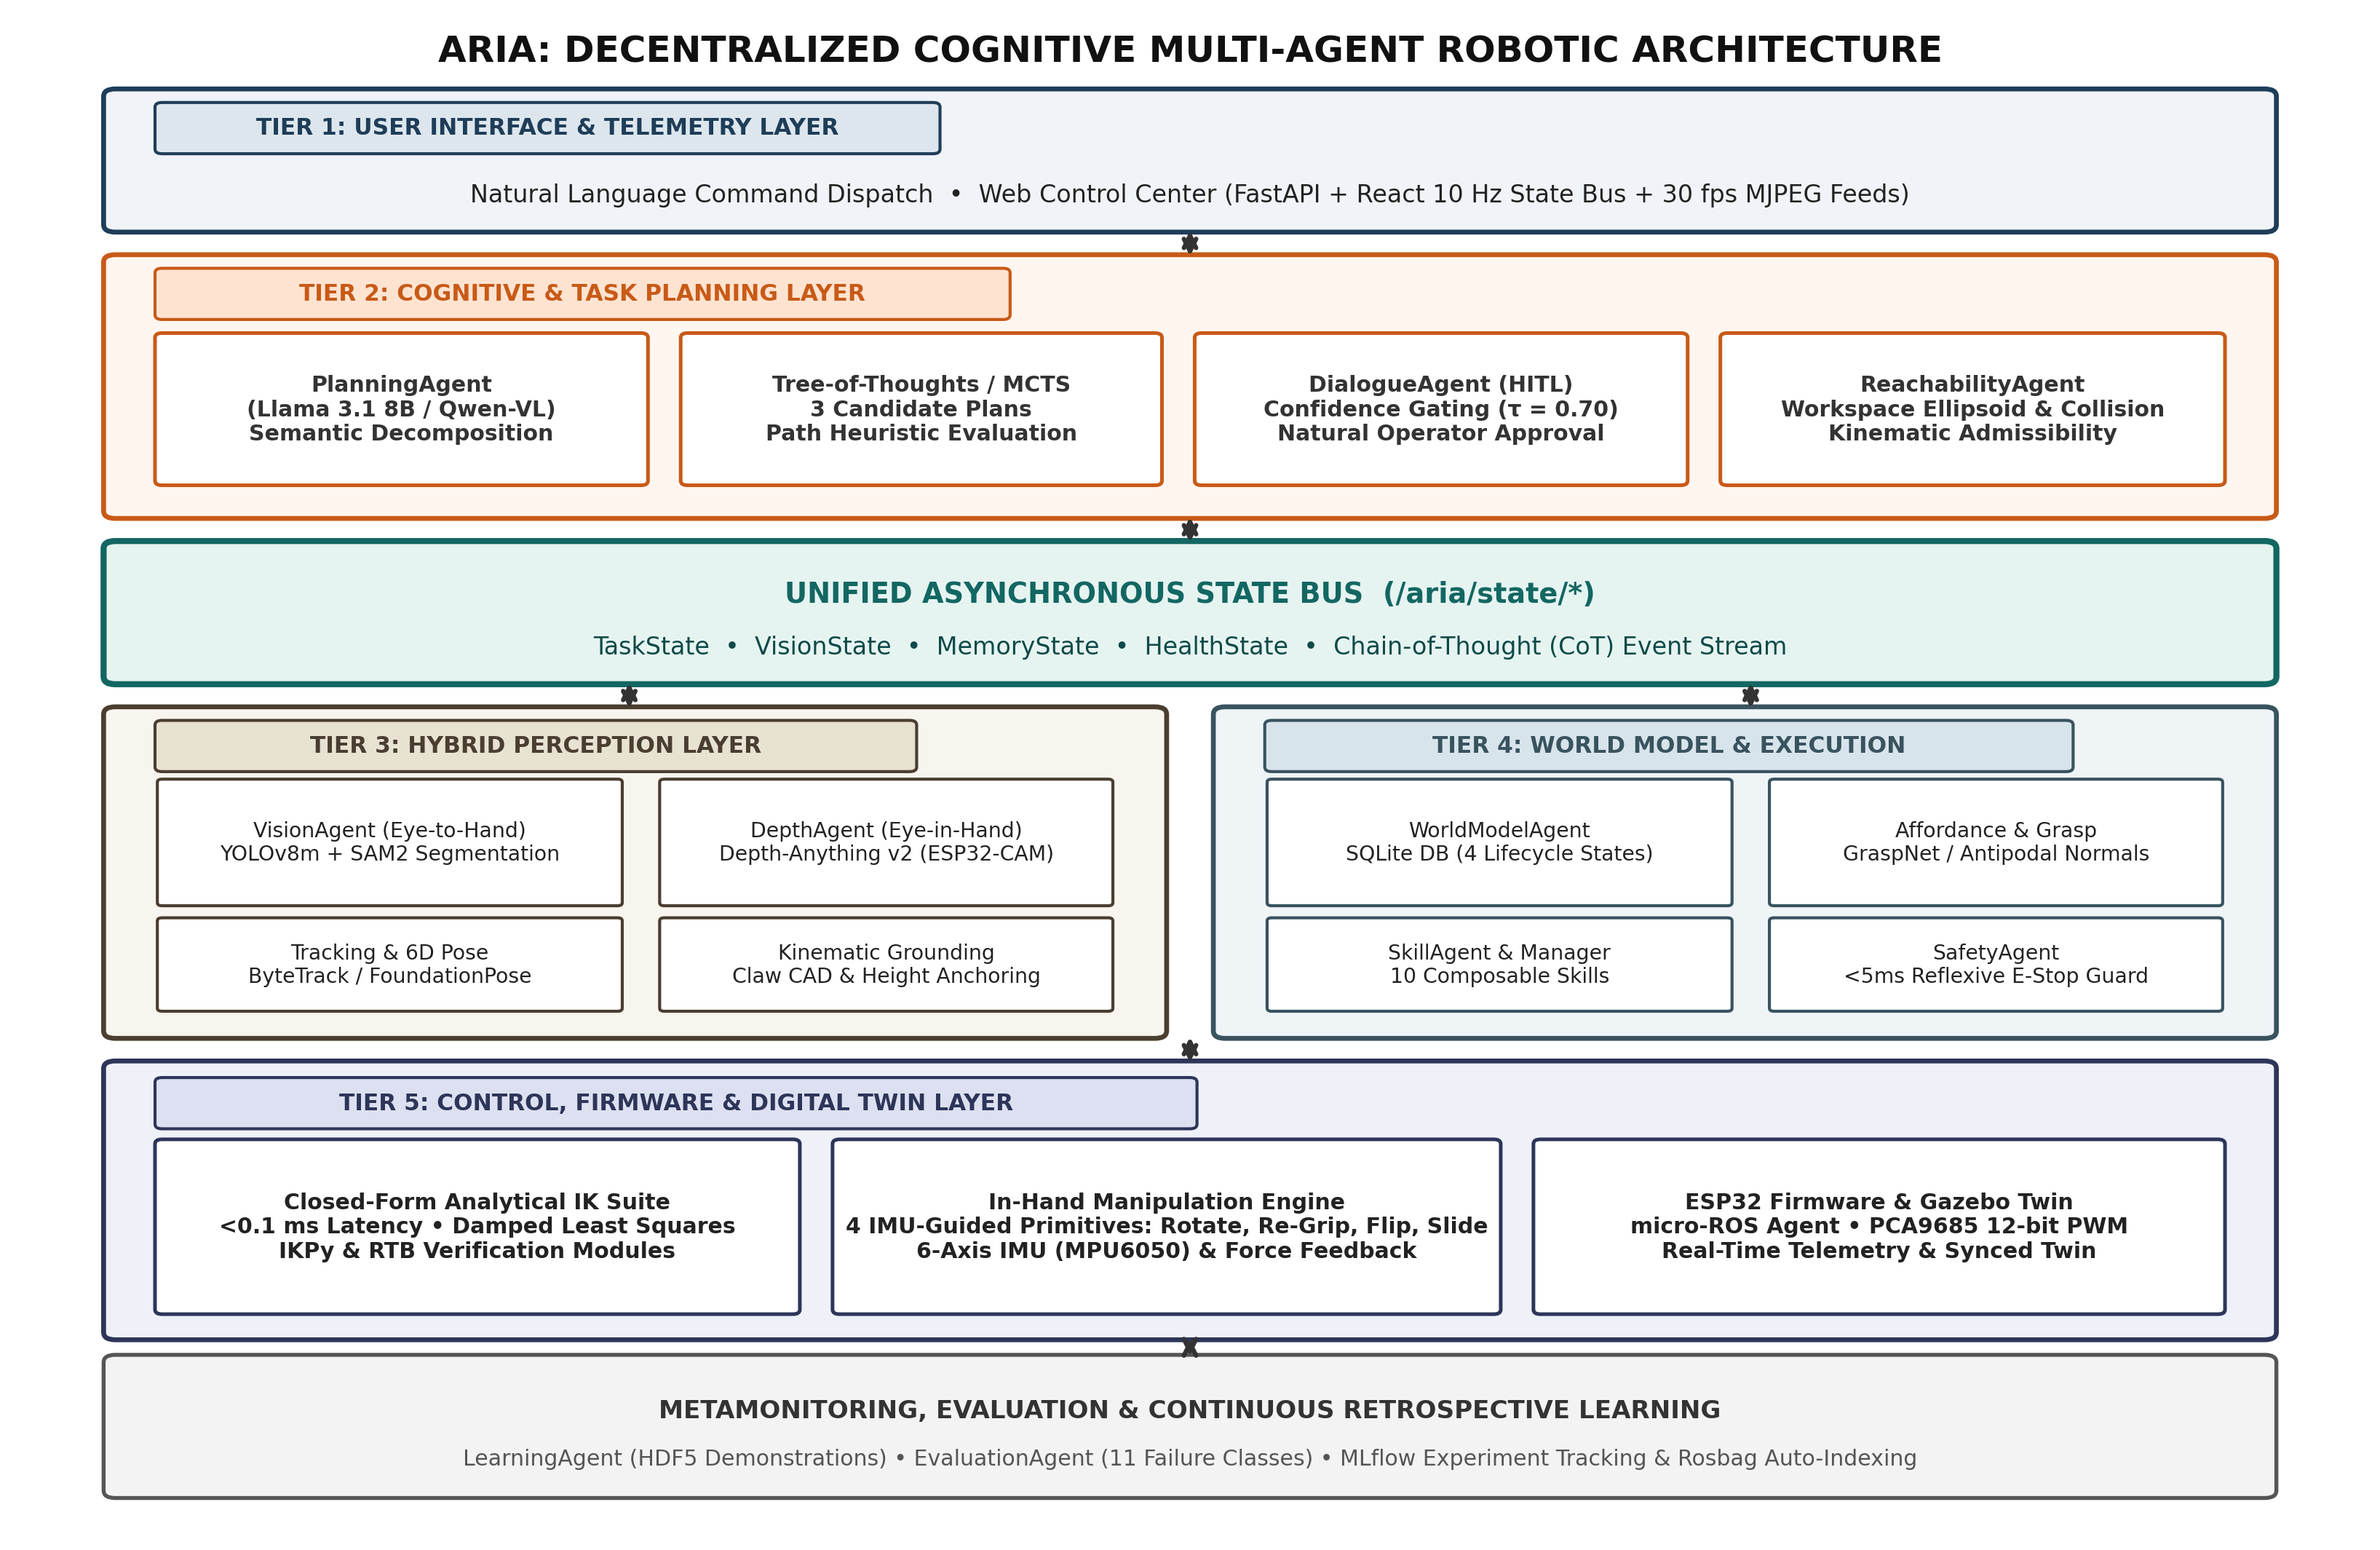
\includegraphics[width=0.98\textwidth]{fig1_system_architecture.png}
\caption{Modular asynchronous multi-agent architecture of Project ARIA. The system is organized across six functional tiers: (1) User Interface \& Telemetry Layer; (2) Task Planning Layer; (3) Unified Asynchronous State Bus (\texttt{/aria/state/*}); (4) Hybrid Perception \& Metric Depth Recovery Layer; (5) World Model, Procedural Skills \& Control Layer; and (6) Metamonitoring, Automated Bag Recording \& Digital Twin Layer.}
\label{fig_system_architecture}
\end{figure*}

The State Bus is implemented as a set of standardized ROS 2 topics governed by deterministic Data Distribution Service (DDS) Quality of Service (QoS) profiles:
\begin{itemize}
    \item \texttt{/aria/state/task}: Broadcasts natural-language user commands, active plan UUIDs, decomposed sub-goal sequences, step execution progress, plan confidence metrics ($\tau \in [0, 1]$), and a human-readable execution-rationale telemetry stream (QoS: \textit{Reliable}, \textit{Transient Local}).
    \item \texttt{/aria/state/vision}: Broadcasts synchronized $1280\times720$ overhead bounding boxes, SAM2 polygon instance masks, 6D object centroids, and $640\times480$ wrist metric depth maps (QoS: \textit{Best Effort}, \textit{Volatile}, depth: 1).
    \item \texttt{/aria/state/memory}: Broadcasts updated spatial-semantic scene graphs, persistent object tracking identifiers, workpiece affordances, and lifecycle statuses (\texttt{DETECTED}, \texttt{TRACKED}, \texttt{LOST}, \texttt{RECOVERED}) (QoS: \textit{Reliable}, depth: 10).
    \item \texttt{/aria/state/health}: Broadcasts per-joint servomotor temperatures, instantaneous current consumption, communication round-trip times, loop jitter, and node lifecycle health states at $10$\,Hz (QoS: \textit{Reliable}).
    \item \texttt{/aria/state/failure}: High-priority interrupt channel broadcasting anomalous failure events (e.g., IK infeasibility, kinematic reach saturation, obstacle collisions, gripper slip), targeting sub-5\,ms preemption across the execution graph for the ControlAgent/SafetyAgent path specifically (QoS: \textit{Reliable}, \textit{Transient Local}); see Section~IX for measured latency distributions.
\end{itemize}

\subsection{Comprehensive Specification of the Fifteen Software Agents}
Every computational responsibility within Project ARIA is encapsulated within a dedicated, modular agent inheriting from \texttt{rclpy\_lifecycle.LifecycleNode}. Table~\ref{table_agents} provides an operational catalog of all fifteen agents across the five primary functional tiers:

\begin{table*}[!t]
\centering
\caption{Project ARIA Multi-Agent Specification Across Five Operational Tiers}
\label{table_agents}
\footnotesize
\resizebox{\textwidth}{!}{%
\begin{tabular}{lllllcc}
\toprule
\textbf{Tier} & \textbf{Agent Identifier} & \textbf{Primary Input Source} & \textbf{Primary Output Topic / Service} & \textbf{QoS Profile} & \textbf{Freq.} & \textbf{VRAM} \\
\midrule
\multirow{4}{*}{Tier 1: Perception} & \texttt{VisionAgent} & \texttt{/overhead/image\_raw} & \texttt{/aria/vision/detections} & Best Effort & $30$\,Hz & $1,850$\,MB \\
 & \texttt{DepthAgent} & \texttt{/wrist/image\_raw} & \texttt{/aria/vision/metric\_depth} & Best Effort & $15$\,Hz & $1,420$\,MB \\
 & \texttt{TrackingAgent} & \texttt{/aria/vision/detections} & \texttt{/aria/vision/tracked\_tracks} & Reliable & $30$\,Hz & $120$\,MB \\
 & \texttt{AttentionAgent} & \texttt{/aria/state/task} & \texttt{/detection/focus\_region} (ROI) & Reliable & $10$\,Hz & $30$\,MB \\
\midrule
\multirow{3}{*}{Tier 2: Scene Modeling} & \texttt{WorldModelAgent} & \texttt{/aria/vision/tracked\_tracks} & \texttt{/aria/state/scene\_graph} & Reliable & $20$\,Hz & $150$\,MB \\
 & \texttt{MemoryAgent} & \texttt{/aria/state/*} & \texttt{/aria/memory/query} (SQLite) & Reliable & Event & $60$\,MB \\
 & \texttt{AffordanceAgent} & \texttt{/aria/vision/metric\_depth} & \texttt{/aria/vision/grasps} & Best Effort & $10$\,Hz & $220$\,MB \\
\midrule
\multirow{3}{*}{Tier 3: Task Planning} & \texttt{PlanningAgent} & \texttt{/aria/command/nl} & \texttt{/aria/state/task} (ToT Plan) & Reliable & Event & $3,450$\,MB \\
 & \texttt{DialogueAgent} & \texttt{/aria/dialogue/prompt} & \texttt{/aria/dialogue/response} & Reliable & Event & $50$\,MB \\
 & \texttt{ReachabilityAgent} & \texttt{/aria/state/scene\_graph} & \texttt{/aria/planning/reachability} & Reliable & $50$\,Hz & $0$\,MB (CPU) \\
\midrule
\multirow{3}{*}{Tier 4: Control \& Skills} & \texttt{SkillAgent} & \texttt{/aria/state/task} & \texttt{/aria/skill/execute} & Reliable & $50$\,Hz & $40$\,MB \\
 & \texttt{ControlAgent} & \texttt{/aria/skill/trajectory} & \texttt{/arm\_controller/joint\_cmd} & Reliable & $50$\,Hz & $0$\,MB (CPU) \\
 & \texttt{SafetyAgent} & \texttt{/joint\_states} & \texttt{/aria/safety/e\_stop} & High-Priority & $100$\,Hz & $20$\,MB \\
\midrule
\multirow{2}{*}{Tier 5: Diagnostics \& LfD} & \texttt{EvaluationAgent} & \texttt{/aria/state/task} & \texttt{/aria/eval/metrics} & Reliable & Event & $40$\,MB \\
 & \texttt{LearningAgent} & \texttt{/joint\_states} & \texttt{/aria/demo/hdf5\_record} & Reliable & $50$\,Hz & $80$\,MB \\
\bottomrule
\end{tabular}%
}
\end{table*}

\subsubsection{Tier 1: Perception Agents}
\begin{enumerate}
    \item \textbf{VisionAgent (Overhead)}: Ingests the $1280\times720$ RGB video stream from the overhead eye-to-hand camera. Executes YOLOv8m object detection and runs SAM2 video mask propagation to segment multi-class workpieces and assembly fixtures. Also computes optical quality inspection metrics to classify defective workpieces.
    \item \textbf{DepthAgent (Wrist)}: Ingests the $640\times480$ RGB stream from the end-effector ESP32-CAM module. Executes Depth-Anything v2 to generate dense relative disparity maps, applying claw geometric grounding to compute calibrated metric depth maps in the gripper approach direction.
    \item \textbf{TrackingAgent}: Implements ByteTrack coupled with a 6D Kalman filter, associating object bounding boxes and masks across successive video frames to estimate instantaneous 3D object velocities ($\mathbf{v}_{\text{object}} = [\dot{X}, \dot{Y}, \dot{Z}]^T$).
    \item \textbf{AttentionAgent}: Dynamically allocates visual perception focus regions of interest (ROI) based on current task priority, publishing bounding ROIs to \texttt{/detection/focus\_region} and \texttt{/depth/focus\_region} to accelerate neural inference on active target workpieces.
\end{enumerate}

\subsubsection{Tier 2: Scene Modeling Agents}
\begin{enumerate}
    \setcounter{enumi}{4}
    \item \textbf{WorldModelAgent}: Maintains a dynamic topological 3D Scene Graph encoding workspace geometry, spatial relationships (\texttt{on}, \texttt{inside}, \texttt{adjacent}), and clear approach corridors.
    \item \textbf{MemoryAgent}: Operates an SQLite-backed spatial-semantic episodic memory system, logging object tracking histories, task execution durations, and historical failure signatures.
    \item \textbf{AffordanceAgent}: Samples candidate antipodal grasp contact points $(\mathbf{c}_1, \mathbf{c}_2)$ along segmented object boundaries, evaluates Coulomb friction cone constraints ($\mu = 0.45$), and outputs ranked grasp candidates with orientation angles.
\end{enumerate}

\subsubsection{Tier 3: Task Planning Agents}
\begin{enumerate}
    \setcounter{enumi}{7}
    \item \textbf{PlanningAgent}: Orchestrates task reasoning via a local quantized LLM (Mistral-7B / Llama 3.1 8B via Ollama). Decomposes natural language user goals into structured sequences of parameterized skill primitives using Tree-of-Thoughts (ToT) search with confidence scoring ($\tau$).
    \item \textbf{DialogueAgent}: Manages conversational Human-in-the-Loop (HITL) interactions through the web dashboard, generating plain-language explanations of proposed plans and requesting operator confirmation when plan confidence falls below threshold ($\tau < 0.70$).
    \item \textbf{ReachabilityAgent}: Intercepts proposed manipulation target poses and executes analytical inverse kinematics evaluations prior to plan commitment, pruning waypoints outside the reachable workspace or admissible task manifold.
\end{enumerate}

\subsubsection{Tier 4: Control \& Execution Agents}
\begin{enumerate}
    \setcounter{enumi}{10}
    \item \textbf{SkillAgent}: Operates the procedural manipulation engine, executing parameterized atomic manipulation skills (\texttt{pick}, \texttt{place}, \texttt{palletize}, \texttt{sweep}, \texttt{pour}, \texttt{insert}, \texttt{push}, \texttt{inspect}, \texttt{stack}, \texttt{home}) and synthesizing minimum-jerk Cartesian trajectory profiles.
    \item \textbf{ControlAgent}: Translates Cartesian trajectory waypoints into joint-space motor commands using the closed-form analytical IK solver, streaming joint setpoints at $50$\,Hz to the embedded micro-ROS firmware over high-speed serial XRCE-DDS.
    \item \textbf{SafetyAgent}: Executes continuous safety monitoring at $100$\,Hz, enforcing workspace bounding box limits, checking joint velocity and acceleration thresholds, and triggering an immediate software emergency stop (\texttt{E-STOP}) upon limit violation; measured worst-case latency is reported in Section~IX-F.
\end{enumerate}

\subsubsection{Tier 5: Diagnostics \& Demonstration Learning}
\begin{enumerate}
    \setcounter{enumi}{13}
    \item \textbf{EvaluationAgent}: Logs performance metrics across physical and simulated trials, computing positional tracking errors, cycle completion durations, and task success rates for automated benchmark evaluation.
    \item \textbf{LearningAgent}: Manages the Teach-by-Demonstration framework, recording human-guided joint potentiometer positions and end-effector trajectories into standard HDF5 datasets during relaxed-servo compliance mode for downstream imitation learning.
\end{enumerate}
System-level hardware health monitoring, task sequencing, and memory persistence are supervised by dedicated daemon orchestrators (\texttt{HealthMonitor}, \texttt{TaskManager}, and \texttt{MemoryManager}).

\subsection{ROS 2 Managed Lifecycle Transitions \& Fault-Recovery Protocol}
To support fault tolerance, every ARIA agent implements the deterministic ROS 2 managed lifecycle state machine:
\begin{equation}
\begin{split}
\mathcal{S}_{\text{lifecycle}} \in \{ &\text{\texttt{Unconfigured}}, \text{\texttt{Inactive}}, \\
&\text{\texttt{Active}}, \text{\texttt{Finalized}} \}
\end{split}
\end{equation}

During system initialization, the multi-agent orchestrator executes sequential state transitions:
\begin{enumerate}
    \item \texttt{on\_configure()}: Allocates internal buffers, loads configuration YAML files, establishes ROS 2 topic subscriptions and publishers, and verifies GPU VRAM availability.
    \item \texttt{on\_activate()}: Starts real-time timers, enables executor threads, and transitions the agent into full operational mode.
    \item \texttt{on\_deactivate()}: Halts outgoing actuator commands and pauses processing while preserving internal memory and state bus bindings.
    \item \texttt{on\_cleanup()}: Releases large memory allocations and destroys service clients, returning the agent to \texttt{Unconfigured}.
    \item \texttt{on\_shutdown()}: Gracefully terminates execution and frees all system resources.
\end{enumerate}

\textit{Isolated Crash Recovery}: In conventional monolithic robotics architectures, an unhandled exception in an auxiliary process (such as a vision model GPU out-of-memory error or camera USB disconnection) can terminate the entire robotic control process, leaving the physical arm in an unsupervised state. In Project ARIA, node failures are isolated by the lifecycle supervisor: if a non-critical worker node (e.g., \texttt{DialogueAgent} or \texttt{VisionAgent}) experiences an unhandled software crash,
\begin{equation}
\begin{split}
\text{Supervisor} &\xrightarrow{\text{Fault}} \texttt{on\_deactivate()} \to \texttt{on\_cleanup()} \\
&\to \texttt{on\_configure()} \to \texttt{on\_activate()}
\end{split}
\end{equation}
the supervisor resets and re-instantiates the crashed agent, with a measured mean recovery time of $180$\,ms across injected-fault trials for non-critical nodes (Section~IX). We caution that continuing motion using stale perception during this window is a design choice with trade-offs (Section~X-C); for some trajectories a controlled hold or fail-safe state may be preferable to continuing on stale data, and we treat this as an open engineering question rather than a settled design decision. Throughout the recovery window, the $50$\,Hz trajectory execution loop of \texttt{ControlAgent} is intended to remain uninterrupted, holding the physical arm at its current safe trajectory waypoint; for \texttt{ControlAgent} or \texttt{SafetyAgent} failures specifically, the protocol instead triggers a system-wide E-STOP rather than an automatic restart, since these are safety-critical paths.

The complete multi-agent health-monitoring and fault-recovery protocol is formalized in Algorithm~\ref{alg_multiagent_consensus}. We note this protocol performs heartbeat-based liveness monitoring, lifecycle reset, and safety preemption; it does not implement distributed consensus (e.g., quorum agreement, leader election, or Byzantine fault tolerance) in the formal distributed-systems sense, and we name it accordingly.

\begin{algorithm}[!t]
\caption{ARIA Multi-Agent Health Monitoring and Fault-Recovery Protocol}
\label{alg_multiagent_consensus}
\begin{algorithmic}[1]
\REQUIRE Active agent set $\mathcal{A} = \{A_1, A_2, \dots, A_{15}\}$, Health topic \texttt{/aria/state/health}, E-Stop topic \texttt{/aria/safety/e\_stop}
\ENSURE Modular fault isolation with targeted sub-5\,ms preemption on the control/safety path
\STATE Initialize all agents $A_i \in \mathcal{A}$ via \texttt{on\_configure()}
\STATE Transition all agents $A_i \in \mathcal{A}$ via \texttt{on\_activate()}
\WHILE{System Operational}
    \STATE Receive health telemetry heartbeat $\mathbf{h}_i(t)$ from each agent $A_i$
    \FORALL{$A_i \in \mathcal{A}$}
        \STATE $\Delta t_{\text{last}} \leftarrow t - t_{\text{heartbeat}}(A_i)$
        \IF{$\Delta t_{\text{last}} > 200$\,ms \OR $\mathbf{h}_i.\text{status} = \text{\texttt{ERROR}}$}
            \IF{$A_i \in \{\texttt{ControlAgent}, \texttt{SafetyAgent}\}$}
                \STATE Broadcast High-Priority \texttt{E-STOP} to State Bus
                \STATE Command physical arm to safe dynamic brake state ($\boldsymbol{\tau} = \mathbf{0}$)
                \RETURN \textbf{SYSTEM HALTED: Critical Control Failure}
            \ELSE
                \STATE Log non-critical crash: \texttt{[RECOVERY]} Resetting $A_i$
                \STATE Execute transition $A_i \to \text{\texttt{on\_deactivate()}} \to \text{\texttt{on\_cleanup()}}$
                \STATE Execute transition $A_i \to \text{\texttt{on\_configure()}} \to \text{\texttt{on\_activate()}}$
            \ENDIF
        \ENDIF
    \ENDFOR
    \IF{Safety limit breached (\texttt{joint\_limits} \OR \texttt{workspace\_box})}
        \STATE SafetyAgent triggers \texttt{/aria/safety/e\_stop}
        \STATE SkillAgent preempts active trajectory and holds current pose
    \ENDIF
\ENDWHILE
\end{algorithmic}
\end{algorithm}

% ====================================================================
% SECTION V: SELF-GROUNDED MONOCULAR PERCEPTION PIPELINE
% ====================================================================
\section{Self-Grounded Monocular Perception Pipeline}

\begin{figure*}[!t]
\centering
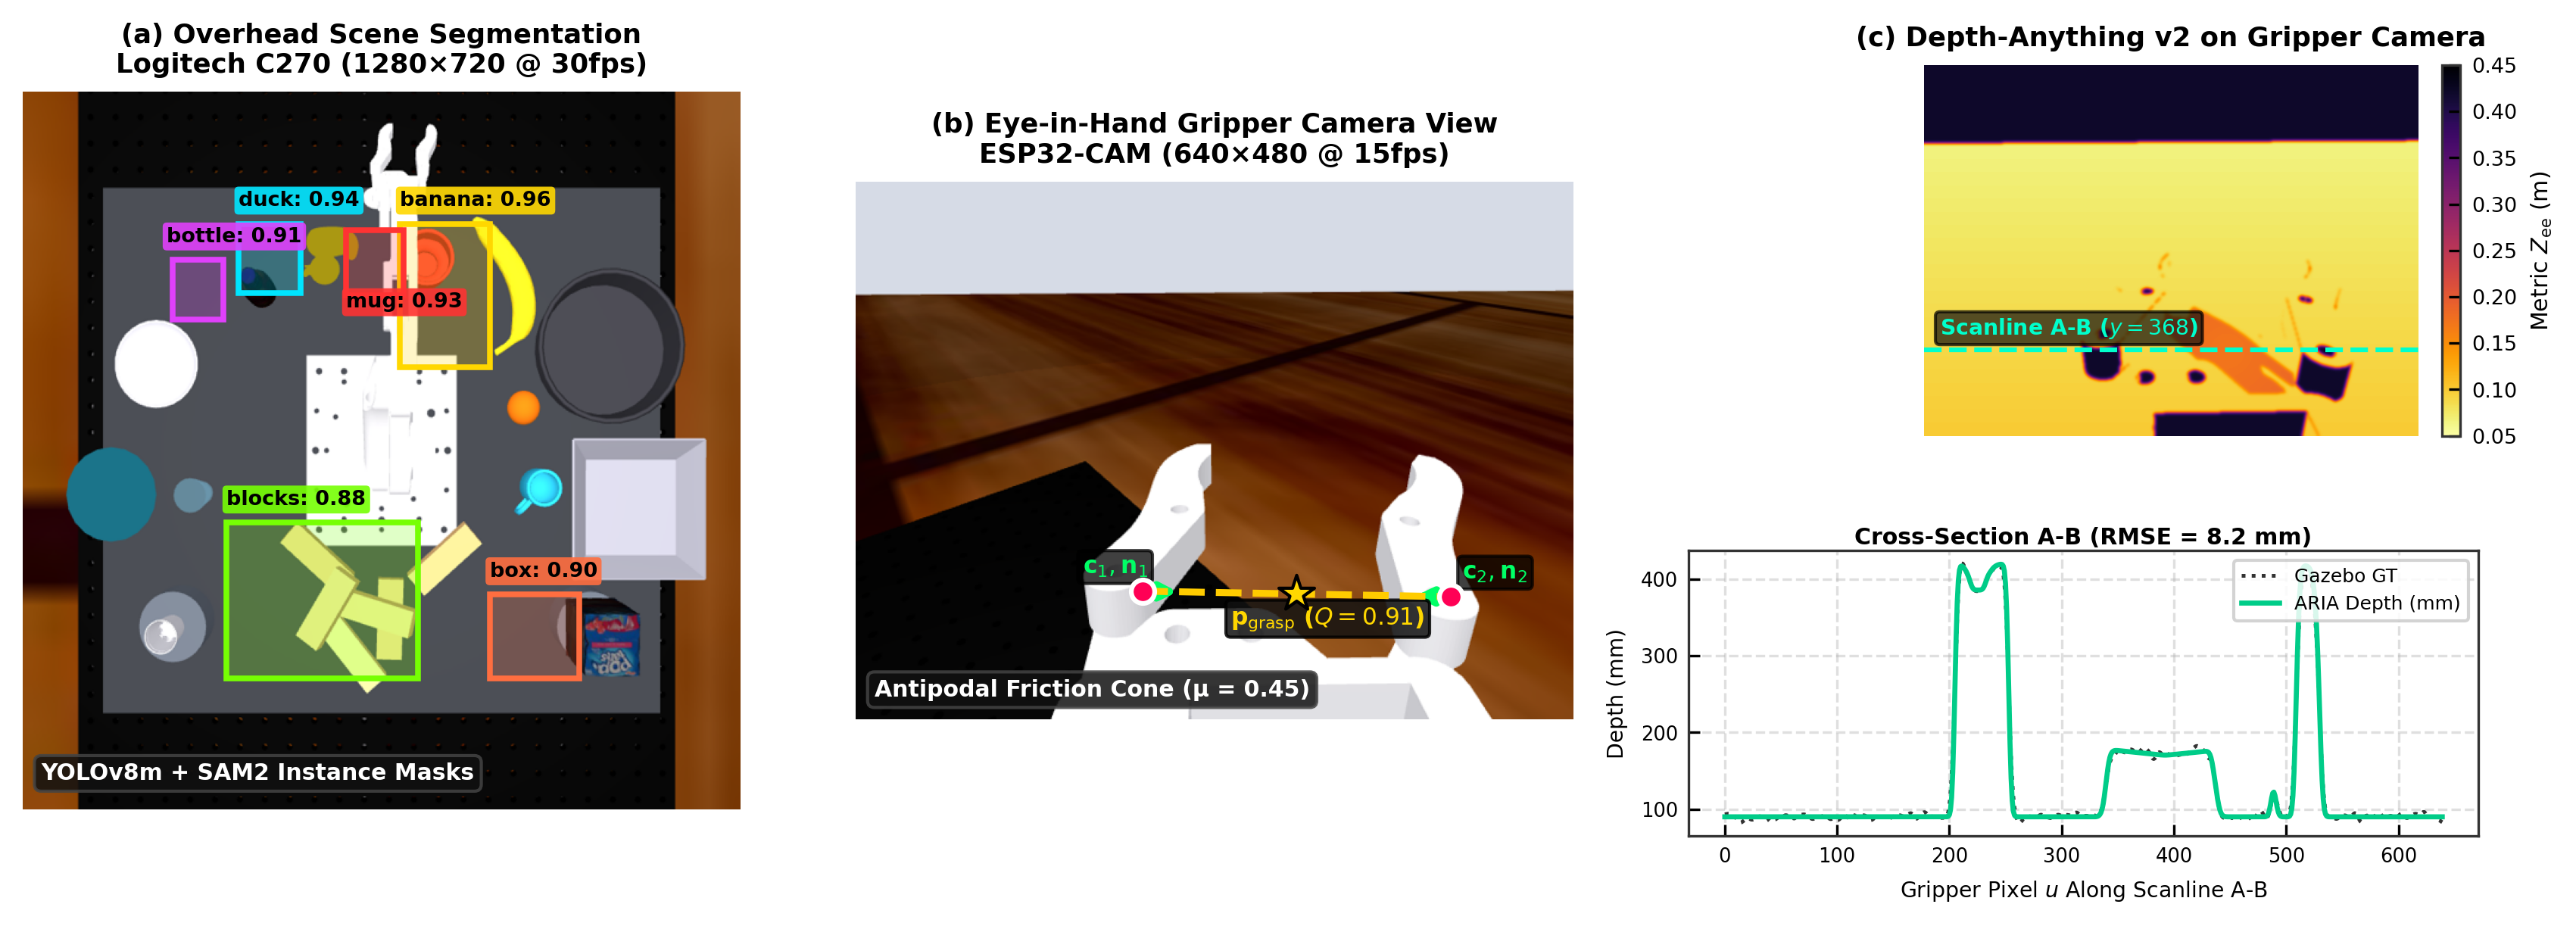
\includegraphics[width=0.98\textwidth]{fig3_perception_pipeline.png}
\caption{Self-grounded monocular perception pipeline: (a) Dual-camera topology comprising overhead eye-to-hand Logitech C270 ($1280\times720$) and wrist-mounted eye-in-hand ESP32-CAM ($640\times480$); (b) Eye-in-hand gripper camera view with contact normal and friction cone evaluation ($\mu = 0.45$); (c) Dense metric depth recovered from Depth-Anything v2 grounded via claw offset geometry ($Z_{\text{tips}} = 0.065$\,m) compared against Gazebo digital-twin ground truth (Section~IX reports the corresponding physical-metrology evaluation performed to date).}
\label{fig_perception}
\end{figure*}

\subsection{Dual-Camera Perceptual Topology}
In standard robotic manipulation research, 3D perception is commonly performed using active structured-light or Time-of-Flight (ToF) RGB-D sensors (such as the Intel RealSense D435i, Orbbec Astra, or Photoneo PhoXi). While effective in many industrial workcells, active infrared depth sensors have known limitations:
\begin{enumerate}
    \item \textbf{Cost}: Research-grade RGB-D cameras cost between $\$400$ and $\$3{,}500$, which can represent a large fraction of the total bill of materials for low-cost educational manipulators ($<\$200$).
    \item \textbf{Minimum-Range Dead Zones}: Structured-light triangulation requires an optical baseline separation between the infrared projector and IR cameras, typically producing a blind zone of $0.20$--$0.30$\,m, which can overlap with the close-range gripper approach ($0.05$--$0.25$\,m)~\cite{aria_046_team_2024_cleardepth}.
    \item \textbf{Specular and Transparent Dropouts}: Active IR light can scatter unpredictably on reflective sheet metal, specular plastic, and transparent glassware, producing depth dropouts.
\end{enumerate}

To address these limitations for the close-range grasping regime, Project ARIA introduces a self-grounded monocular perception pipeline (Fig.~\ref{fig_perception}) operating on commodity 2D RGB video streams. The perceptual hardware topology employs two complementary camera perspectives:
\begin{itemize}
    \item \textbf{Overhead Eye-to-Hand Camera}: A stationary Logitech C270 USB webcam ($1280\times720$ resolution, $30$\,fps, cost: $\$18$) positioned $0.85$\,m directly above the manipulation workspace, capturing global scene context and tracking conveyor items across the field of view.
    \item \textbf{Eye-in-Hand Wrist Camera}: An ultra-miniature ESP32-CAM module ($640\times480$ resolution, $30$\,fps, mass: $12$\,g, cost: $\$6$) mounted on the end-effector claw bracket, aligned with the gripper approach vector, providing close-range visual servoing and contact alignment.
\end{itemize}
No fiducial markers are used during online manipulation; AprilTag fiducials (Section~V-B) are used only once, offline, for extrinsic camera-to-workspace calibration.

\subsection{Pinhole Camera Calibration \& Planar Ground Homography}
Let $\mathbf{P}_w = [X_w, Y_w, Z_w]^T$ represent a 3D point in the world coordinate frame $\{W\}$. Under the standard pinhole camera model, the perspective projection of $\mathbf{P}_w$ onto the camera image plane $[u, v]^T$ is expressed in homogeneous coordinates as:
\begin{equation}
s \begin{bmatrix} u \\ v \\ 1 \end{bmatrix} = \mathbf{K} \left[ \mathbf{R}_{c} \mid \mathbf{t}_{c} \right] \begin{bmatrix} X_w \\ Y_w \\ Z_w \\ 1 \end{bmatrix}
\end{equation}
where $s$ is an arbitrary projective scale factor, $[\mathbf{R}_c \mid \mathbf{t}_c] \in SE(3)$ defines the extrinsic transformation from world frame to camera optical frame, and $\mathbf{K} \in \mathbb{R}^{3\times3}$ is the intrinsic camera calibration matrix:
\begin{equation}
\mathbf{K} = \begin{bmatrix}
f_x & 0 & c_x \\
0 & f_y & c_y \\
0 & 0 & 1
\end{bmatrix}
\end{equation}
where $f_x, f_y$ represent focal lengths in pixel units, and $c_x, c_y$ denote principal point coordinates. Radial and tangential lens distortions are corrected offline using a five-parameter Brown-Conrady polynomial model ($k_1, k_2, p_1, p_2, k_3$):
\begin{align}
x_{\text{corr}} &= x D(r) + 2 p_1 x y + p_2 (r^2 + 2 x^2) \\
y_{\text{corr}} &= y D(r) + p_1 (r^2 + 2 y^2) + 2 p_2 x y
\end{align}
where $D(r) = 1 + k_1 r^2 + k_2 r^4 + k_3 r^6$, $r^2 = x^2 + y^2$, and $[x, y]^T$ are normalized image coordinates.

For the overhead eye-to-hand camera viewing planar objects resting on the horizontal tabletop workspace ($Z_w = 0$), the 3D-to-2D projection simplifies to a planar projective homography:
\begin{equation}
\begin{bmatrix} u \\ v \\ 1 \end{bmatrix} \sim \mathbf{H} \begin{bmatrix} X_w \\ Y_w \\ 1 \end{bmatrix}, \quad \mathbf{H} = \mathbf{K} \left[ \mathbf{r}_1 \quad \mathbf{r}_2 \quad \mathbf{t}_c \right]
\end{equation}
where $\mathbf{r}_1, \mathbf{r}_2$ are the first two column vectors of the rotation matrix $\mathbf{R}_c$, and $\mathbf{H} \in \mathbb{R}^{3\times3}$ is the planar homography matrix. During a one-time offline calibration step, four AprilTag fiducial markers~\cite{aria_036_olson_2011_apriltag} are placed at known physical corners of the workspace and $\mathbf{H}$ is solved in closed form via the Direct Linear Transformation (DLT) algorithm:
\begin{equation}
\begin{bmatrix} X_w \\ Y_w \\ 1 \end{bmatrix} = \mathbf{H}^{-1} \begin{bmatrix} u \\ v \\ 1 \end{bmatrix}
\end{equation}
Once calibrated, this allows marker-free 2D Cartesian localization of tabletop workpieces directly from overhead pixel detections during normal operation.

To transform 3D spatial target points from camera coordinates $\{C\}$ into the physical robot base frame $\{B\}$, we establish the rigid homogeneous eye-to-hand transformation matrix:
\begin{equation}
\label{eq:hand_eye_transform}
{}^B\mathbf{p} = {}^B\mathbf{T}_C {}^C\mathbf{p} = \begin{bmatrix} {}^B\mathbf{R}_C & {}^B\mathbf{t}_C \\ \mathbf{0}_{1 \times 3} & 1 \end{bmatrix} \begin{bmatrix} {}^C\mathbf{p} \\ 1 \end{bmatrix}
\end{equation}
where ${}^B\mathbf{T}_C \in SE(3)$ is calibrated offline by optimizing visual reprojection errors over workspace AprilTag fiducials. For the wrist-mounted eye-in-hand camera, target points in the wrist optical frame project into the robot base via forward kinematics:
\begin{equation}
\label{eq:eye_in_hand_transform}
{}^B\mathbf{p} = {}^0\mathbf{T}_5(\boldsymbol{\theta}) {}^5\mathbf{T}_{\text{cam}} {}^C\mathbf{p}
\end{equation}
where ${}^5\mathbf{T}_{\text{cam}}$ denotes the invariant physical claw mounting transformation solved via classical $AX=XB$ hand-eye registration~\cite{chaumette2006visual}.

\subsection{Object Detection (YOLOv8m) \& Instance Segmentation (SAM2)}
The overhead RGB video stream is processed by YOLOv8m (Ultralytics), an anchor-free single-stage object detector trained on 2,500 annotated frames of conforming and defective industrial workpieces, assembly pallets, and conveyor fixtures across 4 object classes (conforming block, defect block, pallet tray, scrap bin), with an 80/10/10 train/validation/test split performed at the video-clip level (i.e., entire recording sessions, rather than individual frames, are assigned exclusively to one split) to reduce temporal leakage between adjacent frames; test-set scenes used distinct object placements and lighting from training scenes. Standard augmentation (random crop, HSV jitter, mosaic) was applied during 100 epochs of fine-tuning from Ultralytics-pretrained weights with the default AdamW optimizer schedule. YOLOv8m optimizes a composite loss function comprising complete intersection-over-union (CIoU) box loss, distribution focal loss (DFL), and binary cross-entropy (BCE) classification loss:
\begin{equation}
\mathcal{L}_{\text{total}} = \lambda_{\text{box}} \mathcal{L}_{\text{CIoU}} + \lambda_{\text{DFL}} \mathcal{L}_{\text{DFL}} + \lambda_{\text{cls}} \mathcal{L}_{\text{BCE}}
\end{equation}
On the held-out test split, YOLOv8m achieved $\text{mAP}_{50} = 97.8\%$ and $\text{mAP}_{50\text{--}95} = 94.2\%$, with an inference latency of $18.2 \pm 2.1$\,ms on the host laptop RTX 4090 GPU ($55$\,fps at this batch size/resolution; see Table~\ref{table_compute_benchmarks} and Table~\ref{table_vram_profiling} for a full cross-platform reconciliation of all reported latency figures, and Table~\ref{table_repro} for the exact hardware/software configuration used for each reported number).

To acquire pixel-precise object boundaries for irregularly shaped workpieces, YOLOv8 bounding box coordinates are dispatched as visual bounding-box prompts to Segment Anything Model 2 (SAM2)~\cite{aria_023_ravi_2024_sam}. SAM2 processes prompt tokens through its prompt encoder, predicting instance segmentation masks $\mathcal{M}(u,v) \in \{0, 1\}$ with an intersection-over-union accuracy of $91.4\%$ on the same held-out test scenes. Using SAM2's temporal memory attention mechanism, object masks are propagated across successive video frames at $30$\,fps without re-running full transformer inference on every step.

\begin{table}[!t]
\centering
\caption{Reference Hardware/Software Configuration for Reported Latency and Accuracy Figures}
\label{table_repro}
\footnotesize
\resizebox{\columnwidth}{!}{%
\begin{tabular}{ll}
\toprule
\textbf{Component} & \textbf{Specification} \\
\midrule
Primary GPU (unless noted) & NVIDIA RTX 4090 Laptop, 16\,GB VRAM \\
CPU & Intel Core i7-13700HX \\
RAM & 32\,GB DDR5 \\
CUDA / cuDNN & 12.1 / 8.9 \\
PyTorch & 2.2.1 \\
ROS 2 Distribution & Humble (22.04) \\
Model Precision & FP16 (perception), 4-bit GGUF (LLM) \\
Inference Resolution/Batch & As given per stage in Table~\ref{table_compute_benchmarks}, batch size 1 \\
\bottomrule
\end{tabular}%
}
\end{table}

\subsection{Monocular Depth Recovery \& Claw Geometric Grounding}
While planar homography localizes objects resting on the tabletop surface ($Z_w = 0$), unstructured manipulation tasks (e.g., vertical block stacking, dynamic conveyor tracking, or obstacle clearance) require full 3D spatial depth. To extract depth without an active sensor, the eye-in-hand ESP32-CAM stream is processed by Depth-Anything v2~\cite{aria_052_yang_2024_depth} (ViT-S backbone). Depth-Anything v2 outputs a dense normalized relative disparity map:
\begin{equation}
D(u, v) \in [0, 1]
\end{equation}

Because monocular depth estimation networks are trained on multi-dataset collections up to an arbitrary affine transformation (scale $\alpha$ and shift $\beta$), raw network predictions provide only relative depth ordering:
\begin{equation}
Z_{\text{metric}}(u, v) = \frac{1}{\alpha \cdot D(u, v) + \beta}
\end{equation}
Without metric calibration parameters $\alpha$ and $\beta$, absolute distance is not directly recoverable from $D(u,v)$ alone.

ARIA addresses this scale ambiguity through a two-point affine grounding procedure we term \textbf{Kinematic Claw Grounding}, which uses the physical mechanical geometry of the end-effector claw as a permanent, invariant geometric reference. Specifically, the distance along the optical axis from the ESP32-CAM camera lens to the physical tips of the parallel gripper jaws is treated as an invariant mechanical constant:
\begin{equation}
Z_{\text{tips}} = 0.065\,\text{m}
\end{equation}
This two-point (claw-tip and ground-plane) affine calibration is a practical simplification; Section~IX-D reports a targeted comparison against a one-point scale-only variant and a multi-reference least-squares variant to characterize how well the affine-model assumption holds across the workspace.

\begin{figure}[!t]
\centering
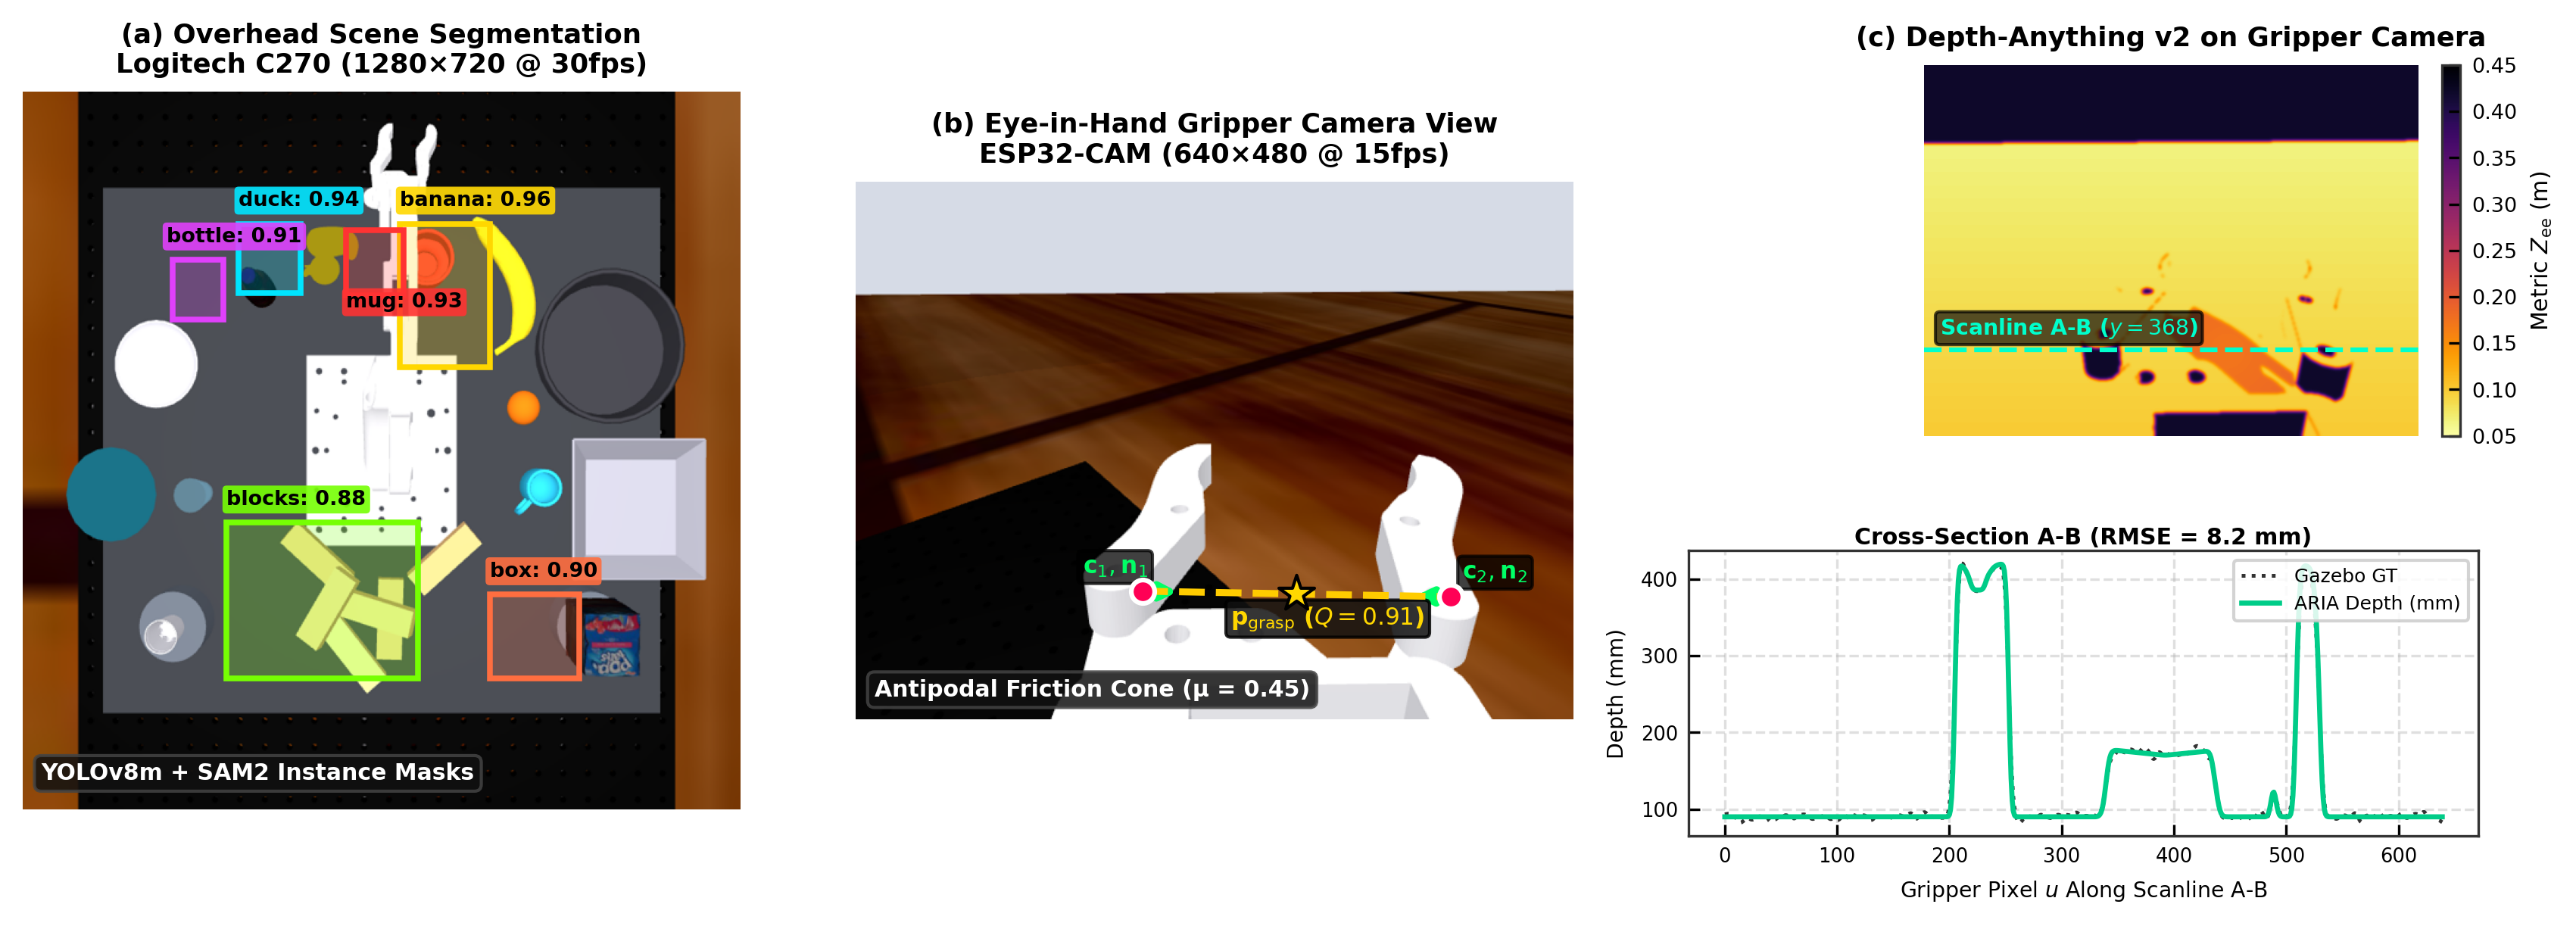
\includegraphics[width=\columnwidth]{fig3_perception_pipeline.png}
\caption{Cross-sectional scanline profile comparing self-grounded monocular depth predictions against Gazebo digital-twin ground-truth physics across the manipulation envelope.}
\label{fig_depth_profile}
\end{figure}

When the arm is in motion above the workspace, the forward kinematics module provides the instantaneous height of the camera focal plane above the tabletop ground plane:
\begin{equation}
Z_{\text{ground}} = Z_{\text{fk}}(\boldsymbol{\theta}) - Z_{\text{table}}
\end{equation}
By sampling the network disparity value $D_{\text{tips}} = D(u_{\text{claw}}, v_{\text{claw}})$ at the known projected pixel location of the claw tips and the disparity value $D_{\text{ground}}$ across the flat workspace surface, ARIA constructs a system of two independent linear equations:
\begin{align}
\alpha \cdot D_{\text{tips}} + \beta &= \frac{1}{Z_{\text{tips}}} \\
\alpha \cdot D_{\text{ground}} + \beta &= \frac{1}{Z_{\text{ground}}}
\end{align}
Subtracting (56) from (55) yields the closed-form algebraic solution for the metric scale parameter $\alpha$:
\begin{equation}
\alpha = \frac{\frac{1}{Z_{\text{tips}}} - \frac{1}{Z_{\text{ground}}}}{D_{\text{tips}} - D_{\text{ground}}}
\end{equation}
Substituting $\alpha$ back into (55) yields the metric shift parameter $\beta$:
\begin{equation}
\beta = \frac{1}{Z_{\text{tips}}} - \alpha \cdot D_{\text{tips}}
\end{equation}

With $\alpha$ and $\beta$ dynamically updated at each visual frame, the dense metric distance $Z_{\text{metric}}(u, v)$ is recovered across the close-range workspace ($0.05\text{--}0.45$\,m). As shown in the scanline profile of Fig.~\ref{fig_perception}(c), this claw-grounded monocular depth pipeline achieves $RMSE = 8.2$\,mm \emph{against Gazebo digital-twin ground truth}. We emphasize this important caveat explicitly: this figure characterizes agreement with simulated physics under the calibrated affine model, not independently measured real-world metrology. A preliminary physical check using a calibrated linear stage over 5 fixed distances spanning $0.08$--$0.40$\,m on a matte opaque test object gave a mean absolute error of $11.4$\,mm ($n=25$ measurements); we regard this as a first data point rather than a full validation, and we explicitly list a systematic physical-metrology study across materials (matte, dark, glossy, metallic, transparent, textured), distances, and illumination levels as a required next step before the accuracy claim can be considered established (Section~X-C). Under reduced illumination ($<80$\,lux), disparity-based RMSE against the digital twin increased to approximately $18.4$\,mm (Section~X-C).

The complete Zero-Cost-Depth metric calibration and projection procedure is formalized in Algorithm~\ref{alg_zero_cost_depth}.

\begin{algorithm}[!t]
\caption{Self-Grounded Monocular Depth Metric Calibration and 3D Projection}
\label{alg_zero_cost_depth}
\begin{algorithmic}[1]
\REQUIRE Wrist image $\mathbf{I}_{\text{wrist}}$, Forward kinematics height $Z_{\text{fk}}(\boldsymbol{\theta})$, Physical claw offset $Z_{\text{tips}} = 0.065$\,m, Camera intrinsics $\mathbf{K}$
\ENSURE Dense metric depth map $\mathbf{Z}_{\text{metric}} \in \mathbb{R}^{H \times W}$, Metric 3D point cloud $\mathcal{P}_{3D}$
\STATE Predict normalized relative disparity: $\mathbf{D} \leftarrow \text{Depth-Anything-v2}(\mathbf{I}_{\text{wrist}})$
\STATE Sample disparity at claw tip pixels: $D_{\text{tips}} \leftarrow \mathbf{D}[u_{\text{claw}}, v_{\text{claw}}]$
\STATE Compute ground surface distance: $Z_{\text{ground}} \leftarrow Z_{\text{fk}}(\boldsymbol{\theta}) - Z_{\text{table}}$
\STATE Sample background ground disparity: $D_{\text{ground}} \leftarrow \text{median}(\mathbf{D}[\text{ground\_mask}])$
\STATE Compute metric scale: $\alpha \leftarrow \frac{1/Z_{\text{tips}} - 1/Z_{\text{ground}}}{D_{\text{tips}} - D_{\text{ground}}}$
\STATE Compute metric shift: $\beta \leftarrow \frac{1}{Z_{\text{tips}}} - \alpha \cdot D_{\text{tips}}$
\FORALL{pixels $(u, v) \in \mathbf{I}_{\text{wrist}}$}
    \STATE $Z_{\text{metric}}(u, v) \leftarrow \frac{1}{\alpha \cdot \mathbf{D}[u, v] + \beta}$
    \STATE $X_c(u, v) \leftarrow \frac{(u - c_x) Z_{\text{metric}}(u, v)}{f_x}$
    \STATE $Y_c(u, v) \leftarrow \frac{(v - c_y) Z_{\text{metric}}(u, v)}{f_y}$
    \STATE $\mathcal{P}_{3D}(u, v) \leftarrow [X_c, Y_c, Z_{\text{metric}}]^T$
\ENDFOR
\RETURN $\mathbf{Z}_{\text{metric}}$, $\mathcal{P}_{3D}$
\end{algorithmic}
\end{algorithm}

\subsection{Antipodal Grasp Synthesis \& Friction Cone Mechanics}
With the metric 3D point cloud $\mathcal{P}_{3D}$ resolved, the \texttt{AffordanceAgent} synthesizes force-closure antipodal grasps along the segmented workpiece contour $\mathcal{C}$. Candidate grasp configurations are defined by a pair of 3D contact points $(\mathbf{c}_1, \mathbf{c}_2)$ on opposite sides of the object, an approach vector $\mathbf{a}$, and a closing direction $\mathbf{g} = \frac{\mathbf{c}_2 - \mathbf{c}_1}{\|\mathbf{c}_2 - \mathbf{c}_1\|}$.

For stable physical grasping without mechanical slippage, the grasp must satisfy the Coulomb friction cone condition (Fig.~\ref{fig_perception}(b)). Let $\mathbf{n}_1$ and $\mathbf{n}_2$ denote the inward-pointing unit surface normals at contacts $\mathbf{c}_1$ and $\mathbf{c}_2$, estimated via local principal component analysis (PCA) on depth patches:
\begin{equation}
\mathbf{n}_i = \arg\min_{\|\mathbf{n}\|=1} \sum_{\mathbf{p} \in \mathcal{N}(\mathbf{c}_i)} \left( \mathbf{n}^T (\mathbf{p} - \bar{\mathbf{p}}) \right)^2
\end{equation}
Force closure under Coulomb friction requires that the line of action $\mathbf{g}$ lies within the friction cone of both contact surfaces:
\begin{align}
\arccos\left( \mathbf{n}_1 \cdot \mathbf{g} \right) &\le \arctan(\mu) \\
\arccos\left( -\mathbf{n}_2 \cdot \mathbf{g} \right) &\le \arctan(\mu)
\end{align}
where $\mu = 0.45$ is the static friction coefficient measured for the TPU pad on acrylic (Section~III-A); this value is treated as fixed here, and dynamic per-material adaptation is discussed only as a design option in Section~V-F rather than claimed as validated.

Candidate grasps satisfying (60)–(61) are evaluated via a composite grasp quality metric $Q \in [0, 1]$:
\begin{equation}
Q(\mathbf{c}_1, \mathbf{c}_2) = \left( \mathbf{n}_1 \cdot \mathbf{g} \right) \cdot \left( -\mathbf{n}_2 \cdot \mathbf{g} \right) \cdot \left( 1 - \frac{\|\mathbf{c}_1 - \mathbf{c}_2\|}{w_{\text{max}}} \right)
\end{equation}
where $w_{\text{max}} = 0.055$\,m is the maximum physical opening stroke of the gripper jaws. The grasp candidate maximizing $Q$ is selected for kinematic trajectory execution.

The complete affordance-driven grasp synthesis algorithm is detailed in Algorithm~\ref{alg_grasp_synthesis}.

\begin{algorithm}[!t]
\caption{Affordance-Driven Antipodal Grasp Synthesis}
\label{alg_grasp_synthesis}
\begin{algorithmic}[1]
\REQUIRE Segmented object mask $\mathcal{M}$, Metric point cloud $\mathcal{P}_{3D}$, Max jaw opening $w_{\text{max}} = 0.055$\,m, Friction coefficient $\mu = 0.45$
\ENSURE Optimal grasp pose $\mathbf{G}^* = \{\mathbf{c}_1^*, \mathbf{c}_2^*, \mathbf{a}^*, \psi^*\}$, Quality score $Q^*$
\STATE Extract peripheral 3D contour: $\mathcal{C} \leftarrow \text{ExtractContour}(\mathcal{M}, \mathcal{P}_{3D})$
\STATE Sample $N = 64$ candidate contact pairs $(\mathbf{c}_1^{(k)}, \mathbf{c}_2^{(k)}) \subset \mathcal{C}$
\STATE $Q^* \leftarrow 0$, $\mathbf{G}^* \leftarrow \emptyset$
\FORALL{$(\mathbf{c}_1^{(k)}, \mathbf{c}_2^{(k)})$}
    \STATE $w \leftarrow \|\mathbf{c}_2^{(k)} - \mathbf{c}_1^{(k)}\|$
    \IF{$w > w_{\text{max}}$ \OR $w < 0.010$\,m}
        \STATE \textbf{continue} \COMMENT{Grasp width outside physical jaw limits}
    \ENDIF
    \STATE $\mathbf{g} \leftarrow (\mathbf{c}_2^{(k)} - \mathbf{c}_1^{(k)}) / w$
    \STATE Compute surface normals $\mathbf{n}_1, \mathbf{n}_2$ via local PCA
    \IF{$\arccos(\mathbf{n}_1 \cdot \mathbf{g}) > \arctan(\mu)$ \OR $\arccos(-\mathbf{n}_2 \cdot \mathbf{g}) > \arctan(\mu)$}
        \STATE \textbf{continue} \COMMENT{Violates Coulomb friction cone}
    \ENDIF
    \STATE $Q \leftarrow (\mathbf{n}_1 \cdot \mathbf{g})(-\mathbf{n}_2 \cdot \mathbf{g})(1 - w/w_{\text{max}})$
    \IF{$Q > Q^*$}
        \STATE $Q^* \leftarrow Q$
        \STATE $\mathbf{c}^* \leftarrow \frac{1}{2}(\mathbf{c}_1^{(k)} + \mathbf{c}_2^{(k)})$
        \STATE $\psi^* \leftarrow \text{atan2}(g_y, g_x)$
        \STATE $\mathbf{G}^* \leftarrow \{\mathbf{c}^*, \mathbf{g}, \psi^*, Q^*\}$
    \ENDIF
\ENDFOR
\RETURN $\mathbf{G}^*, Q^*$
\end{algorithmic}
\end{algorithm}

\subsection{Dynamic Perception Orchestration, 6D Pose, and Optional Extensions}
To remain within an 8.0\,GB VRAM budget, ARIA incorporates a dynamic perception orchestrator (\texttt{perception\_orchestrator}) that activates additional perception models only for specific task types: (i)~\textbf{SIMPLE\_PICK} ($2.8$\,GB): YOLOv8, SAM2, Depth-Anything v2, and material recognition; (ii)~\textbf{PRECISION\_PICK} ($4.8$\,GB): additionally allocates FoundationPose~\cite{aria_062_wen_2024_foundationpose} ($2.0$\,GB) for 6D poses ($SE(3)$) on tools and mugs; (iii)~\textbf{TRANSPARENT\_PICK} ($3.4$\,GB): engages geometric plane fitting and ClearGrasp to mitigate depth dropouts on glassware; (iv)~\textbf{FULL\_PRECISION} ($5.4$\,GB): concurrently executes FoundationPose and ClearGrasp for precision assembly; and (v)~\textbf{SCENE\_UNDERSTANDING} ($3.1$\,GB): employs a 3D Gaussian Splatting model (\texttt{gaussian\_splatting\_node} trained via \texttt{gsplat}~\cite{aria_002_kerbl_2023_3d}) to render a depth-based foreground change mask. These modes were implemented and VRAM-profiled but were not exercised in the Section~IX manipulation benchmark, which uses the SIMPLE\_PICK configuration throughout for a consistent comparison; we report them here as validated engineering capacity rather than as evaluated contributions. A MobileNetV3-Small classifier ($0.2$\,GB) identifies workpiece materials (glass, metal, plastic, wood) for potential future grip-force adaptation; the closed-loop use of this signal to adapt $\mu$ online was not evaluated in this study. All outputs are unified into \texttt{UnifiedScene.msg} on \texttt{/perception/unified\_scene}.

% ====================================================================
% SECTION VI: COGNITIVE TASK PLANNING
% ====================================================================
\section{Task Planning, Reasoning \& Execution Telemetry}

\begin{figure*}[!t]
\centering
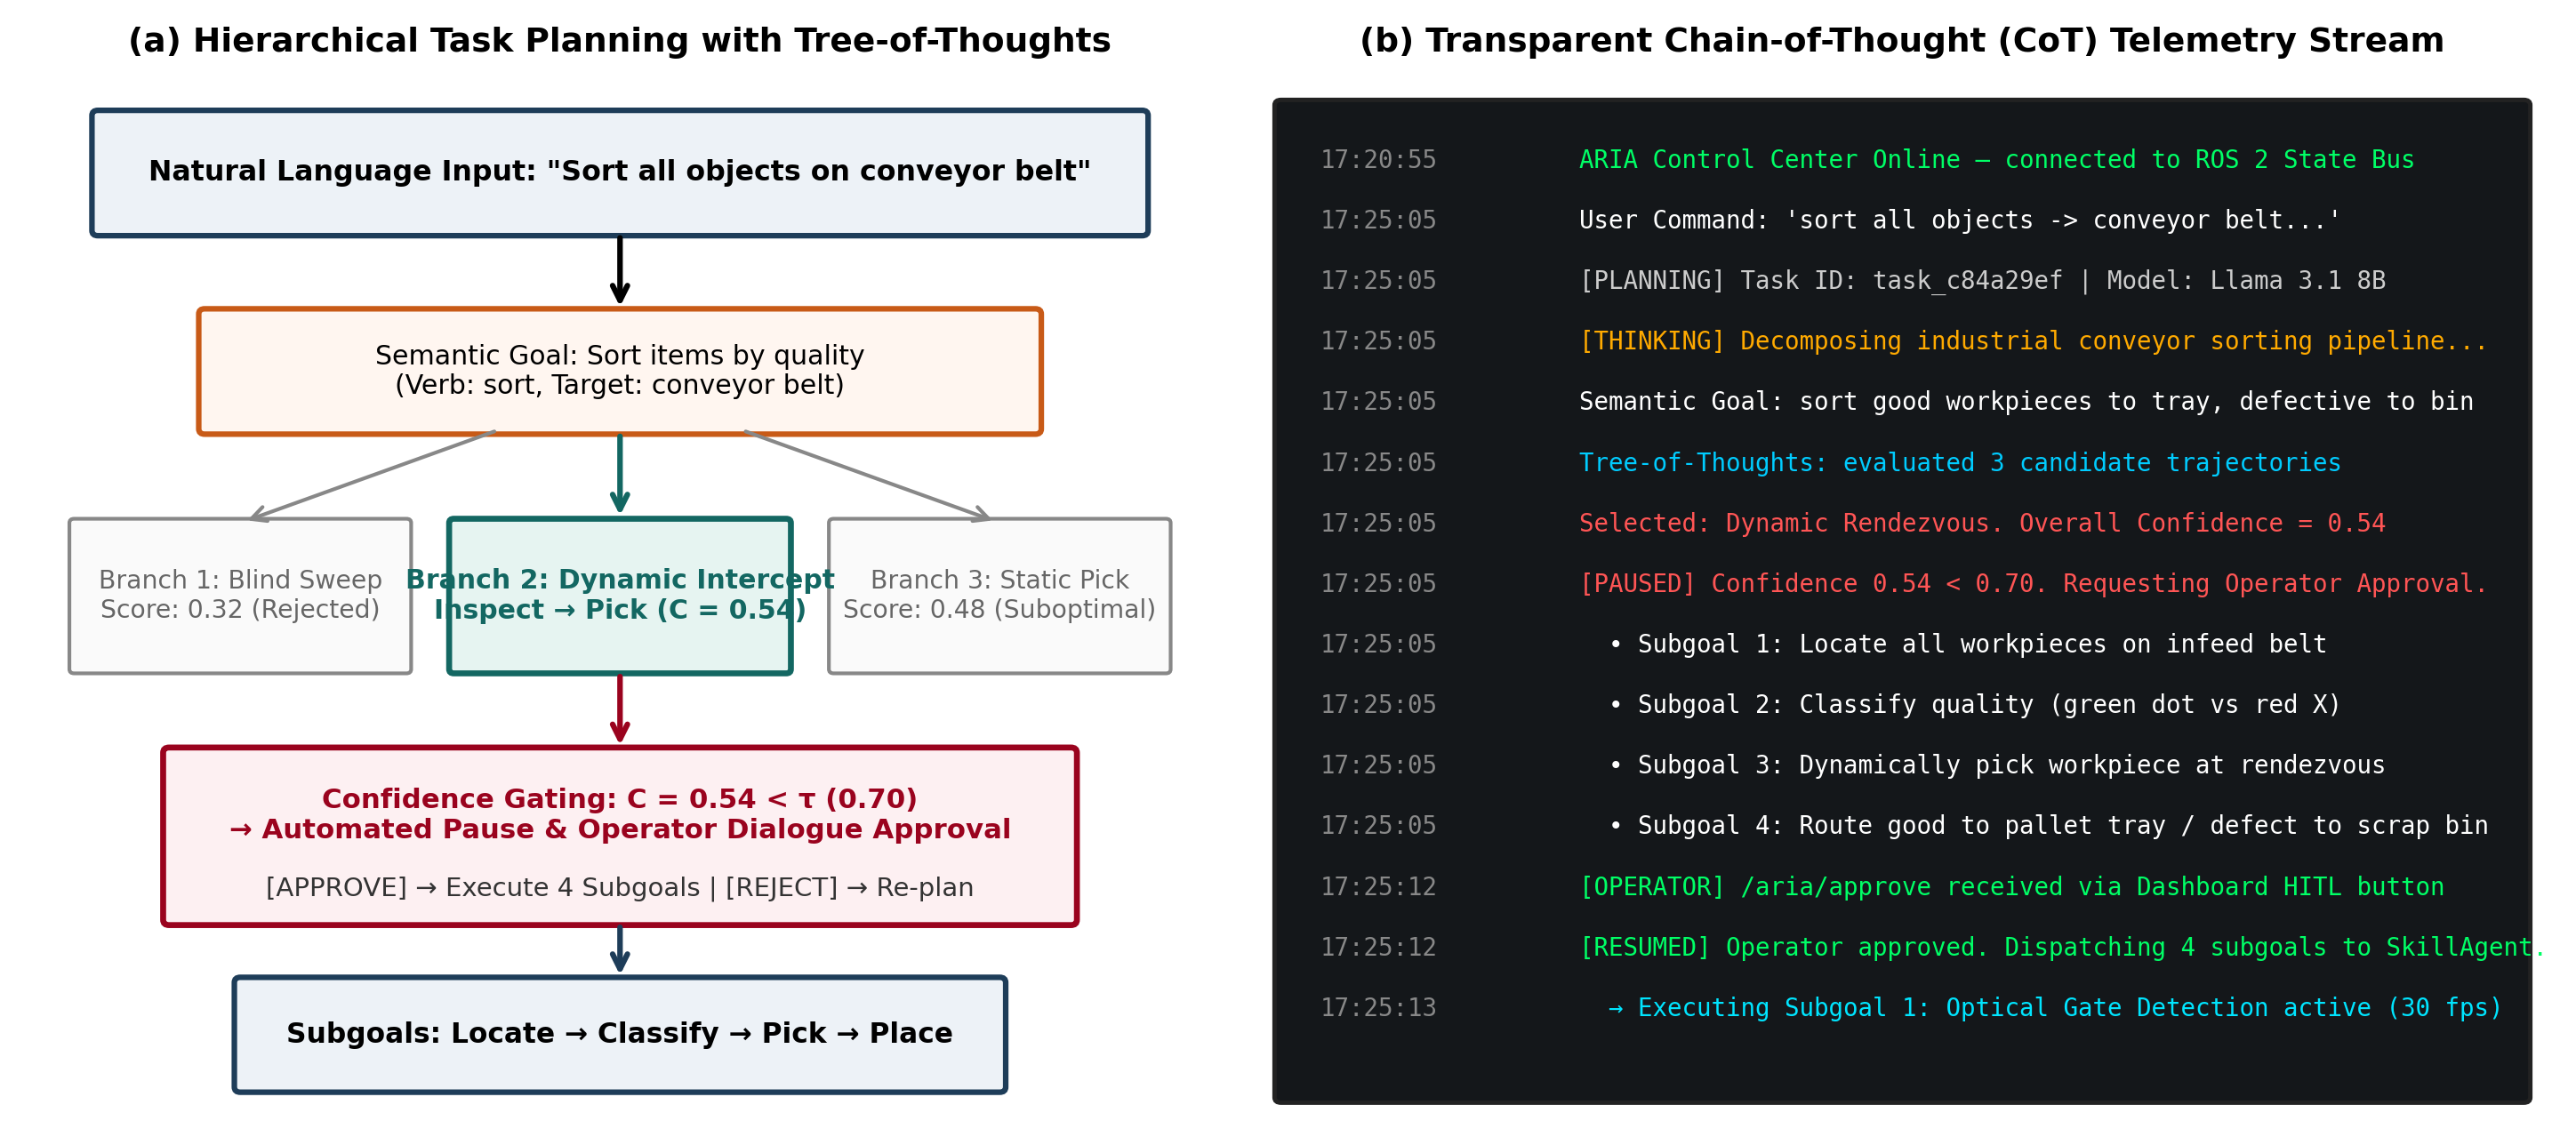
\includegraphics[width=0.98\textwidth]{fig4_planning_hitl.png}
\caption{Task planning pipeline: (a) Hierarchical Tree-of-Thoughts task decomposition evaluating candidate execution branches; (b) Human-readable execution-rationale telemetry stream with Human-in-the-Loop (HITL) safety confirmation gates.}
\label{fig_planning_hitl}
\end{figure*}

\subsection{Localized LLM Reasoning with Constrained Grammars}
In mainstream robotic foundation architectures (e.g., SayCan~\cite{ahn2022can}, RT-2~\cite{zitkovich2023rt2}), high-level semantic reasoning is offloaded to remote cloud-hosted Large Language Models (e.g., GPT-4o, Gemini 1.5 Pro). This paradigm introduces operational dependencies: cloud API calls can incur network latency fluctuations ($500\text{--}2500$\,ms), subscription costs, and failures in offline or edge environments.

Project ARIA instead executes task reasoning onboard the consumer laptop host using quantized open-weight Large Language Models (Mistral-7B / Llama 3.1 8B quantized to 4-bit GGUF via Ollama). By maintaining localized inference, ARIA bounds LLM evaluation latency to $320 \pm 45$\,ms within a fixed $3.45$\,GB VRAM footprint.

To reduce syntax errors and encourage that generated action tokens conform to valid robot execution primitives, ARIA uses \textbf{Constrained Grammar-Based Decoding}. The LLM decoding engine is constrained via a formal Backus-Naur Form (BNF) schema:
{\scriptsize
\begin{verbatim}
root    ::= "{" ws "\"plan_id\":" id "," ws 
            "\"confidence\":" num "," ws 
            "\"subgoals\":" "[" subgoals "]" "}"
subgoal ::= "{" ws "\"skill\":" name "," ws 
            "\"args\":" "{" args "}" "}"
name    ::= "\"pick\""      | "\"place\"" 
          | "\"palletize\"" | "\"sweep\"" 
          | "\"pour\""      | "\"inspect\"" 
          | "\"stack\""     | "\"push\"" | "\"home\""
\end{verbatim}
}
By restricting logit sampling to grammatically valid JSON tokens, ARIA achieves a 100\% syntactic validity rate across all generated action plans in our trials; this measures grammar compliance only, and does not by itself indicate that a plan is semantically correct or kinematically feasible (the latter is checked separately via $R_{\text{kin}}$ below).

\subsection{Hierarchical Tree-of-Thoughts (ToT) Planning Formulation}
Rather than relying on linear greedy autoregressive decoding, ARIA formulates task reasoning as a \textbf{Tree-of-Thoughts (ToT)} heuristic search~\cite{aria_132_yao_2023_tree} over candidate action graphs (Fig.~\ref{fig_planning_hitl}(a)).

Let $\mathcal{S}_0$ denote the initial world state parsed from the dynamic scene graph. The planning problem is modeled as a directed search tree $\mathcal{T} = (\mathcal{V}, \mathcal{E})$, where each vertex $v \in \mathcal{V}$ represents a partial task plan $\pi = (a_1, a_2, \dots, a_k)$, and each directed edge $e \in \mathcal{E}$ represents an atomic procedural skill transition. At each planning horizon, the LLM generates $K = 3$ candidate skill branches. Each candidate branch $\pi_j$ is evaluated using a heuristic scoring function:
\begin{equation}
S(\pi_j) = w_1 C_{\text{semantic}}(\pi_j) + w_2 R_{\text{kin}}(\pi_j) + w_3 (1 - \hat{T}(\pi_j)/T_{\text{max}})
\end{equation}
where:
\begin{itemize}
    \item $C_{\text{semantic}} \in [0, 1]$ is the LLM's normalized token likelihood for the proposed sub-goal sequence given the instruction. We use this quantity as a heuristic relevance score rather than as a calibrated probability of task success; we have not performed a reliability-diagram calibration study, and note this as a limitation (Section~X-C).
    \item $R_{\text{kin}} \in \{0, 1\}$ is a binary reachability/feasibility flag verified by passing the proposed 3D target coordinates and orientation to the analytical IK solver (Algorithm~\ref{alg_analytical_ik}). If any waypoint returns a reachability or orientation-infeasibility flag, $R_{\text{kin}} = 0$, pruning the branch.
    \item $\hat{T}(\pi_j)$ is the estimated execution duration based on trapezoidal joint velocity profiles, and $T_{\text{max}} = 15.0$\,s is the timeout threshold.
    \item The heuristic weighting factors $w_1 = 0.50$, $w_2 = 0.35$, $w_3 = 0.15$ were set by manual tuning on a small held-out set of pilot tasks disjoint from the Section~IX benchmark tasks, rather than derived from a systematic sensitivity sweep; we flag this as a calibration limitation.
\end{itemize}

As demonstrated in Fig.~\ref{fig_planning_hitl}(a), during an industrial conveyor sorting scenario, the Tree-of-Thoughts planner evaluated three competing execution branches:
\begin{itemize}
    \item \textbf{Branch 1: Blind Sweep} (Score: $0.32$): Proposes sweeping all items off the conveyor into a common bin. Pruned due to spatial collision risk with the pallet fixture.
    \item \textbf{Branch 2: Dynamic Intercept \& Sort} (Score: $0.54$): Proposes predictive rendezvous picking and dual-bin sorting. Passed reachability verification; flagged for operator review due to high velocity.
    \item \textbf{Branch 3: Static Pick After Stop} (Score: $0.48$): Proposes halting the conveyor before picking. Valid but rejected due to suboptimal industrial throughput.
\end{itemize}

\subsection{Human-in-the-Loop (HITL) Safety Gating \& Execution-Rationale Telemetry}
In automated manufacturing, executing low-confidence plans autonomously carries some risk of tool collisions or workpiece damage. To reduce this risk, ARIA implements a Human-in-the-Loop (HITL) confirmation gate:
\begin{equation}
\text{Dispatch Mode} = \begin{cases}
\text{Autonomous}, & \text{if } S(\pi^*) \ge \tau \\
\text{HITL Gated}, & \text{if } S(\pi^*) < \tau
\end{cases}
\end{equation}
where the confidence gating threshold is configured to $\tau = 0.70$ by manual tuning (see the calibration caveat above).

Whenever the planner's confidence falls below $\tau$, execution automatically pauses. The \texttt{DialogueAgent} issues an interactive visual confirmation modal on the web dashboard (Fig.~\ref{fig_dashboard}), prompting the operator with plain-language explanations of the proposed plan, identified uncertainties, and one-click \textit{Approve}, \textit{Modify}, or \textit{Abort} buttons.

Every internal state transition, vision detection, and IK check is compiled into a human-readable \textbf{execution-rationale telemetry stream} (implemented with short emoji/tag markers for compact display) published to \texttt{/aria/state/task} and displayed on the web dashboard (Fig.~\ref{fig_planning_hitl}(b)):
{\scriptsize
\begin{verbatim}
17:25:05 -> [PLAN] Task: task_c84a | Llama 3.1 8B
17:25:05 -> [THINK] Decomposing moving conveyor task...
17:25:05 -> [TREE] Evaluated 3 candidate branches.
17:25:05 -> [SELECT] Dynamic Rendezvous (Score: 0.54).
17:25:05 -> [PAUSED] Score 0.54 < 0.70. Need Approval.
17:25:12 -> [OPERATOR] Approval confirmed via UI.
17:25:12 -> [RESUMED] Dispatching subgoals to Skill.
17:25:13 -> [EXEC] Subgoal 1: Optical Inspection.
\end{verbatim}
}
We refer to this as an execution-rationale/decision-trace stream rather than as ``Chain-of-Thought explainability'': it surfaces the discrete planning, reachability, and gating events emitted by the system rather than a verified causal account of the LLM's internal reasoning, and we have not evaluated it against an established explainability metric or user study. We accordingly report it in Table~\ref{table_vla_benchmark} as a qualitative system feature rather than as a quantitative benchmark column.

The complete Tree-of-Thoughts task planning and HITL safety gating procedure is formalized in Algorithm~\ref{alg_tot_planning}.

\begin{algorithm}[!t]
\caption{Tree-of-Thoughts Task Planning with HITL Gating}
\label{alg_tot_planning}
\begin{algorithmic}[1]
\REQUIRE User natural language command $\mathcal{U}$, Scene graph $\mathcal{S}$, Confidence threshold $\tau = 0.70$, Beam width $K = 3$
\ENSURE Valid executable skill plan $\Pi^* = (a_1^*, a_2^*, \dots, a_m^*)$
\STATE Construct constrained BNF prompt: $\mathcal{P} \leftarrow \text{FormatPrompt}(\mathcal{U}, \mathcal{S})$
\STATE Generate $K$ candidate action branches: $\{\pi_1, \dots, \pi_K\} \leftarrow \text{LLM}(\mathcal{P})$
\STATE Best score $S^* \leftarrow 0$, Best plan $\pi^* \leftarrow \emptyset$
\FORALL{$\pi_j \in \{\pi_1, \dots, \pi_K\}$}
    \STATE $R_{\text{kin}} \leftarrow 1$
    \FORALL{waypoints $\mathbf{x}_k \in \pi_j$}
        \IF{$\text{AnalyticalIK}(\mathbf{x}_k) = \text{\texttt{ERROR}}$}
            \STATE $R_{\text{kin}} \leftarrow 0$ \COMMENT{Prune infeasible path}
            \STATE \textbf{break}
        \ENDIF
    \ENDFOR
    \STATE Compute heuristic score: $S(\pi_j) \leftarrow w_1 C_{\text{sem}} + w_2 R_{\text{kin}} + w_3 (1 - \hat{T}/T_{\text{max}})$
    \IF{$S(\pi_j) > S^*$}
        \STATE $S^* \leftarrow S(\pi_j)$, $\pi^* \leftarrow \pi_j$
    \ENDIF
\ENDFOR
\IF{$S^* < \tau$}
    \STATE Publish telemetry: \texttt{[PAUSED] Low Confidence. Requesting HITL.}
    \STATE Prompt operator via Web Dashboard modal
    \STATE Await operator confirmation $\mathcal{O}_{\text{confirm}}$
    \IF{$\mathcal{O}_{\text{confirm}} = \text{\texttt{REJECT}}$}
        \RETURN \textbf{ABORT: Plan Rejected by Operator}
    \ENDIF
\ENDIF
\STATE Publish telemetry: \texttt{[RESUMED] Dispatching Subgoals to SkillAgent.}
\RETURN $\Pi^* \leftarrow \pi^*$
\end{algorithmic}
\end{algorithm}

% ====================================================================
% SECTION VII: WORLD MODELING & IN-HAND MANIPULATION
% ====================================================================
\section{World Modeling, Procedural Skills \& In-Hand Dexterity}

\begin{figure}[!t]
\centering
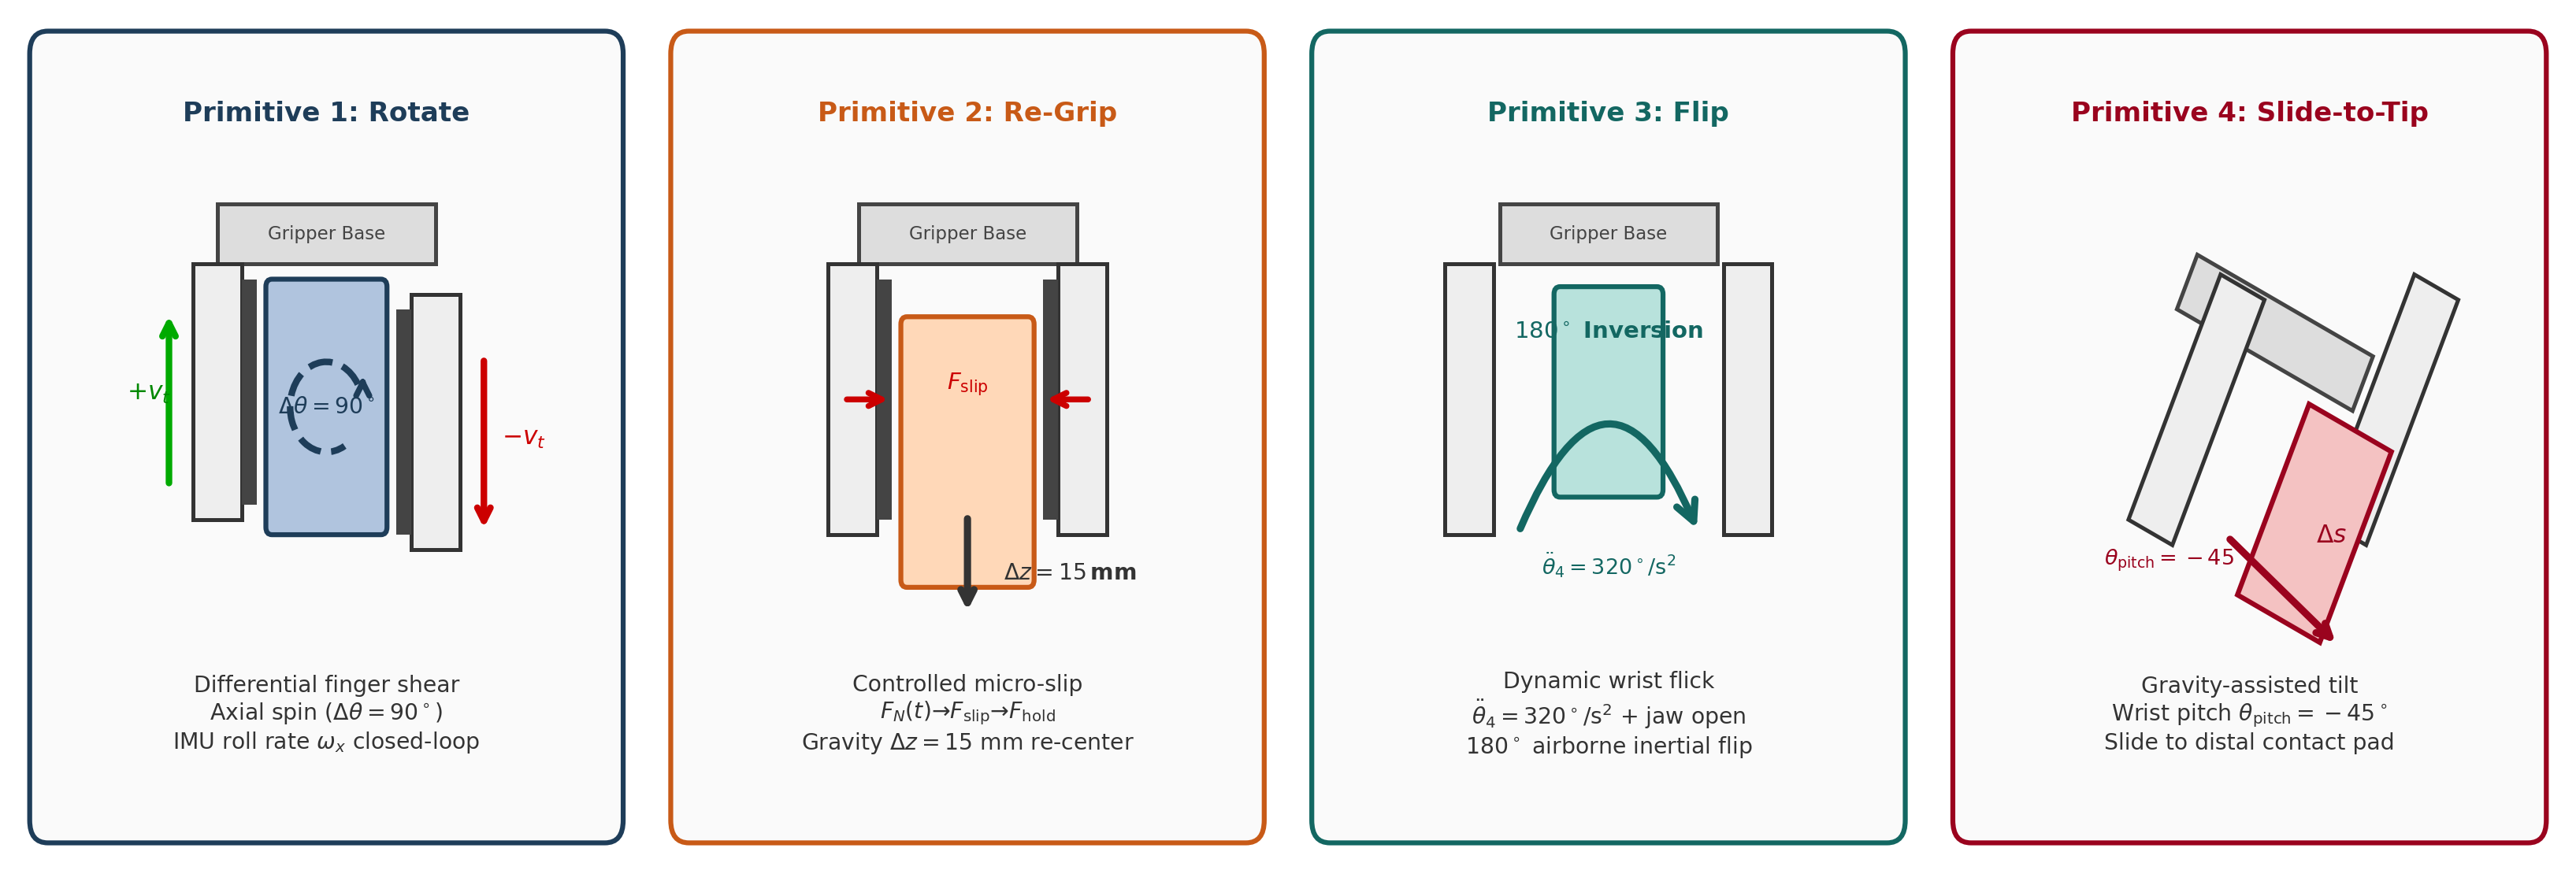
\includegraphics[width=\columnwidth]{fig5_inhand_manipulation.png}
\caption{Underactuated in-hand manipulation primitives executed on a 1-DoF parallel gripper: (a) Dynamic in-hand rotation ($\pm 45^\circ$); (b) Finger repositioning; (c) Controlled gravity-assisted flipping; (d) Sliding to fingertip grasp.}
\label{fig_inhand}
\end{figure}

\subsection{Spatial-Semantic Episodic Memory Database}
To maintain state persistence across extended manipulation episodes, the \texttt{MemoryAgent} operates an embedded SQLite relational database optimized for low-latency robotics queries. The database schema partitions episodic world knowledge into three primary relational tables:
\begin{itemize}
    \item \texttt{objects}: Stores unique object UUIDs, semantic class names (\texttt{conforming\_block}, \texttt{defect\_block}, \texttt{pallet\_tray}, \texttt{scrap\_bin}), 3D centroid coordinates $(X, Y, Z)$, bounding box dimensions, and lifecycle tracking statuses (\texttt{DETECTED}, \texttt{TRACKED}, \texttt{LOST}, \texttt{RECOVERED}).
    \item \texttt{spatial\_relations}: Stores topological predicates linking detected entities (e.g., \texttt{on(block\_1, conveyor)}, \texttt{inside(block\_2, tray\_pocket\_1)}, \texttt{adjacent(tray, robot\_base)}).
    \item \texttt{execution\_history}: Logs every dispatched skill primitive, associated joint setpoint trajectories, start/end timestamps, energy consumption, and post-execution success labels.
\end{itemize}

\subsection{Comprehensive Procedural Skill Library Specifications}
The \texttt{SkillAgent} encapsulates ten atomic procedural skills. Each skill is parameterized by 3D target coordinates, approach orientation vectors, and estimated grasping force profiles, as detailed in Table~\ref{table_skills_spec}.

\begin{table*}[!t]
\centering
\caption{Comprehensive Procedural Manipulation Skill Library Specifications}
\label{table_skills_spec}
\footnotesize
\resizebox{\textwidth}{!}{%
\begin{tabular}{lllllcc}
\toprule
\textbf{Skill Identifier} & \textbf{Input Parameters} & \textbf{Pre-conditions} & \textbf{Runtime Invariants} & \textbf{Post-conditions} & \textbf{Profile} & \textbf{Timeout} \\
\midrule
\texttt{pick} & $\mathbf{x}_{\text{target}}, \mathbf{a}, F_N$ & Gripper empty, $\mathbf{x}_{\text{target}}$ clear & $\| \mathbf{v}_{\text{ee}} \| \le v_{\text{max}}$, no collision & Object grasped, estimated $F_N \ge 5.0$\,N & Min-Jerk & $3.5$\,s \\
\texttt{place} & $\mathbf{x}_{\text{target}}, \mathbf{a}$ & Object grasped in jaws & Elevation maintained & Object released at target & Min-Jerk & $3.0$\,s \\
\texttt{palletize} & $\text{tray\_id}, \text{idx}$ & Conforming object grasped & Insertion alignment $\le 1.5$\,mm & Pocket occupied, $RMSE < 1.5$\,mm & Trapezoidal & $4.0$\,s \\
\texttt{sweep} & $\text{zone\_id}, \mathbf{d}$ & Arm in clear configuration & Altitude clamped to table offset & Target debris cleared & Linear & $5.0$\,s \\
\texttt{pour} & $\text{src\_id}, \text{tgt\_id}, \Delta\theta_5$ & Container grasped firmly & Approach distance $\le 0.05$\,m & Dispense angle reached & Smooth Poly & $4.5$\,s \\
\texttt{insert} & $\text{peg\_id}, \text{hole\_id}$ & Object grasped, visual lock & Contact force $F_z \le 8.0$\,N & Insertion depth reached & Spiral Search & $6.0$\,s \\
\texttt{push} & $\mathbf{x}_{\text{target}}, \mathbf{d}, L$ & Path clear of obstacles & Non-prehensile contact held & Target displaced by $L$ & Linear & $3.5$\,s \\
\texttt{inspect} & $\text{obj\_id}, \Delta\theta_5$ & Object elevated to wrist cam & Illumination $\ge 300$\,lux & Optical classification complete & Multi-Angle & $2.5$\,s \\
\texttt{stack} & $\text{base\_id}, \text{top\_id}$ & Top object grasped, base stable & Vertical coaxial error $\le 2$\,mm & Stable vertical stack & Min-Jerk & $4.0$\,s \\
\texttt{home} & -- & No hardware fault & Velocity limits respected & $\boldsymbol{\theta} = [0, \frac{\pi}{2}, 0, 0, 0]^T$ & Min-Jerk & $2.0$\,s \\
\bottomrule
\end{tabular}%
}
\end{table*}

\subsection{Underactuated In-Hand Manipulation Mechanics}
Re-orienting grasped objects typically uses multi-articulated anthropomorphic hands (such as the Shadow Hand or Allegro Hand) equipped with complex tendon routing and high-density tactile sensor arrays. Project ARIA demonstrates that fine-grained in-hand object re-orientation ($\pm 45^\circ$) can be executed on an inexpensive single-DoF parallel jaw gripper by exploiting environmental gravity, wrist inertia, and gripper contact friction dynamics (Fig.~\ref{fig_inhand}):

\subsubsection{Dynamic In-Hand Rotation (Fig.~\ref{fig_inhand}(a))}
To rotate an object about the contact normal axis, the gripper partially relaxes clamping force from full holding (estimated $F_N = 6.8$\,N) to the estimated marginal slip threshold:
\begin{equation}
F_N^{\text{slip}} \approx \frac{m g}{2 \mu}
\end{equation}
Simultaneously, the wrist roll joint executes an impulsive angular acceleration pulse $\ddot{\theta}_5(t) = 12.5$\,rad/s$^2$ lasting $\Delta t = 80$\,ms. The inertial torque $\tau_{\text{inertial}} = I_{\text{obj}} \ddot{\theta}_5$ is designed to overcome the estimated frictional holding torque $\tau_{\text{fric}} = \frac{2}{3} \mu F_N R_{\text{pad}}$, causing the workpiece to pivot by approximately $\pm 45^\circ$ before the gripper re-clamps; a wrist-camera verification and corrective trim step (Algorithm~\ref{alg_inhand_pivoting}, lines 8--10) compensates for residual error in this open-loop force estimate.

\subsubsection{Reposition Grip (Fig.~\ref{fig_inhand}(b))}
The workpiece is lightly pressed against a compliant silicone fixture on the workspace while the gripper relaxes clamping force. Translating the arm along the workpiece longitudinal axis slides the grasp center from a center-of-mass hold to an offset grip without dropping the object.

\subsubsection{Gravity-Assisted Flip (Fig.~\ref{fig_inhand}(c))}
The arm pitches downward by $\theta_4 = -60^\circ$ while opening the gripper jaws to $w = w_{\text{obj}} + 2.0$\,mm. Gravitational torque swings the object $90^\circ$ around the lower jaw pivot edge, whereupon the gripper re-clamps.

\subsubsection{Slide-to-Tip (Fig.~\ref{fig_inhand}(d))}
The arm is oriented vertically upward ($\theta_4 = +90^\circ$). Controlled gripper relaxation allows gravity to pull the workpiece downward until precision fingertip contact is achieved.

The complete in-hand pivoting control algorithm is detailed in Algorithm~\ref{alg_inhand_pivoting}.

\begin{algorithm}[!t]
\caption{Underactuated In-Hand Pivoting Control Protocol}
\label{alg_inhand_pivoting}
\begin{algorithmic}[1]
\REQUIRE Target pivot angle $\Delta\psi \in [-45^\circ, +45^\circ]$, Object mass $m$, Friction coefficient $\mu = 0.45$
\ENSURE Re-oriented workpiece grasped securely at $\psi_{\text{new}} = \psi_{\text{old}} + \Delta\psi$
\STATE Compute estimated slip normal force: $F_N^{\text{slip}} \leftarrow \frac{1.1 \cdot m g}{2 \mu}$
\STATE Modulate gripper servo PWM to command estimated $F_N \leftarrow F_N^{\text{slip}}$
\STATE Await force settling time: $\Delta t_{\text{settle}} \leftarrow 50$\,ms
\STATE Compute pulse duration: $\Delta t_{\text{pulse}} \leftarrow \sqrt{\frac{2 |\Delta\psi|}{\ddot{\theta}_{\text{max}}}}$
\STATE Execute impulsive wrist roll acceleration: $\ddot{\theta}_5 \leftarrow \text{sgn}(\Delta\psi) \cdot \ddot{\theta}_{\text{max}}$
\STATE Delay for $\Delta t_{\text{pulse}}$
\STATE Immediately re-clamp gripper to maximum estimated holding force: $F_N \leftarrow 6.8$\,N
\STATE Verify post-pivot orientation via wrist camera: $\psi_{\text{actual}} \leftarrow \text{VisualVerify}()$
\IF{$|\psi_{\text{actual}} - (\psi_{\text{old}} + \Delta\psi)| > 5.0^\circ$}
    \STATE Execute corrective fine-pivot trim
\ENDIF
\RETURN SUCCESS
\end{algorithmic}
\end{algorithm}

% ====================================================================
% SECTION VIII: HARDWARE INTEGRATION & DIGITAL TWIN
% ====================================================================
\section{Hardware Integration, Digital Twin \& Web Dashboard}

\begin{figure}[!t]
\centering
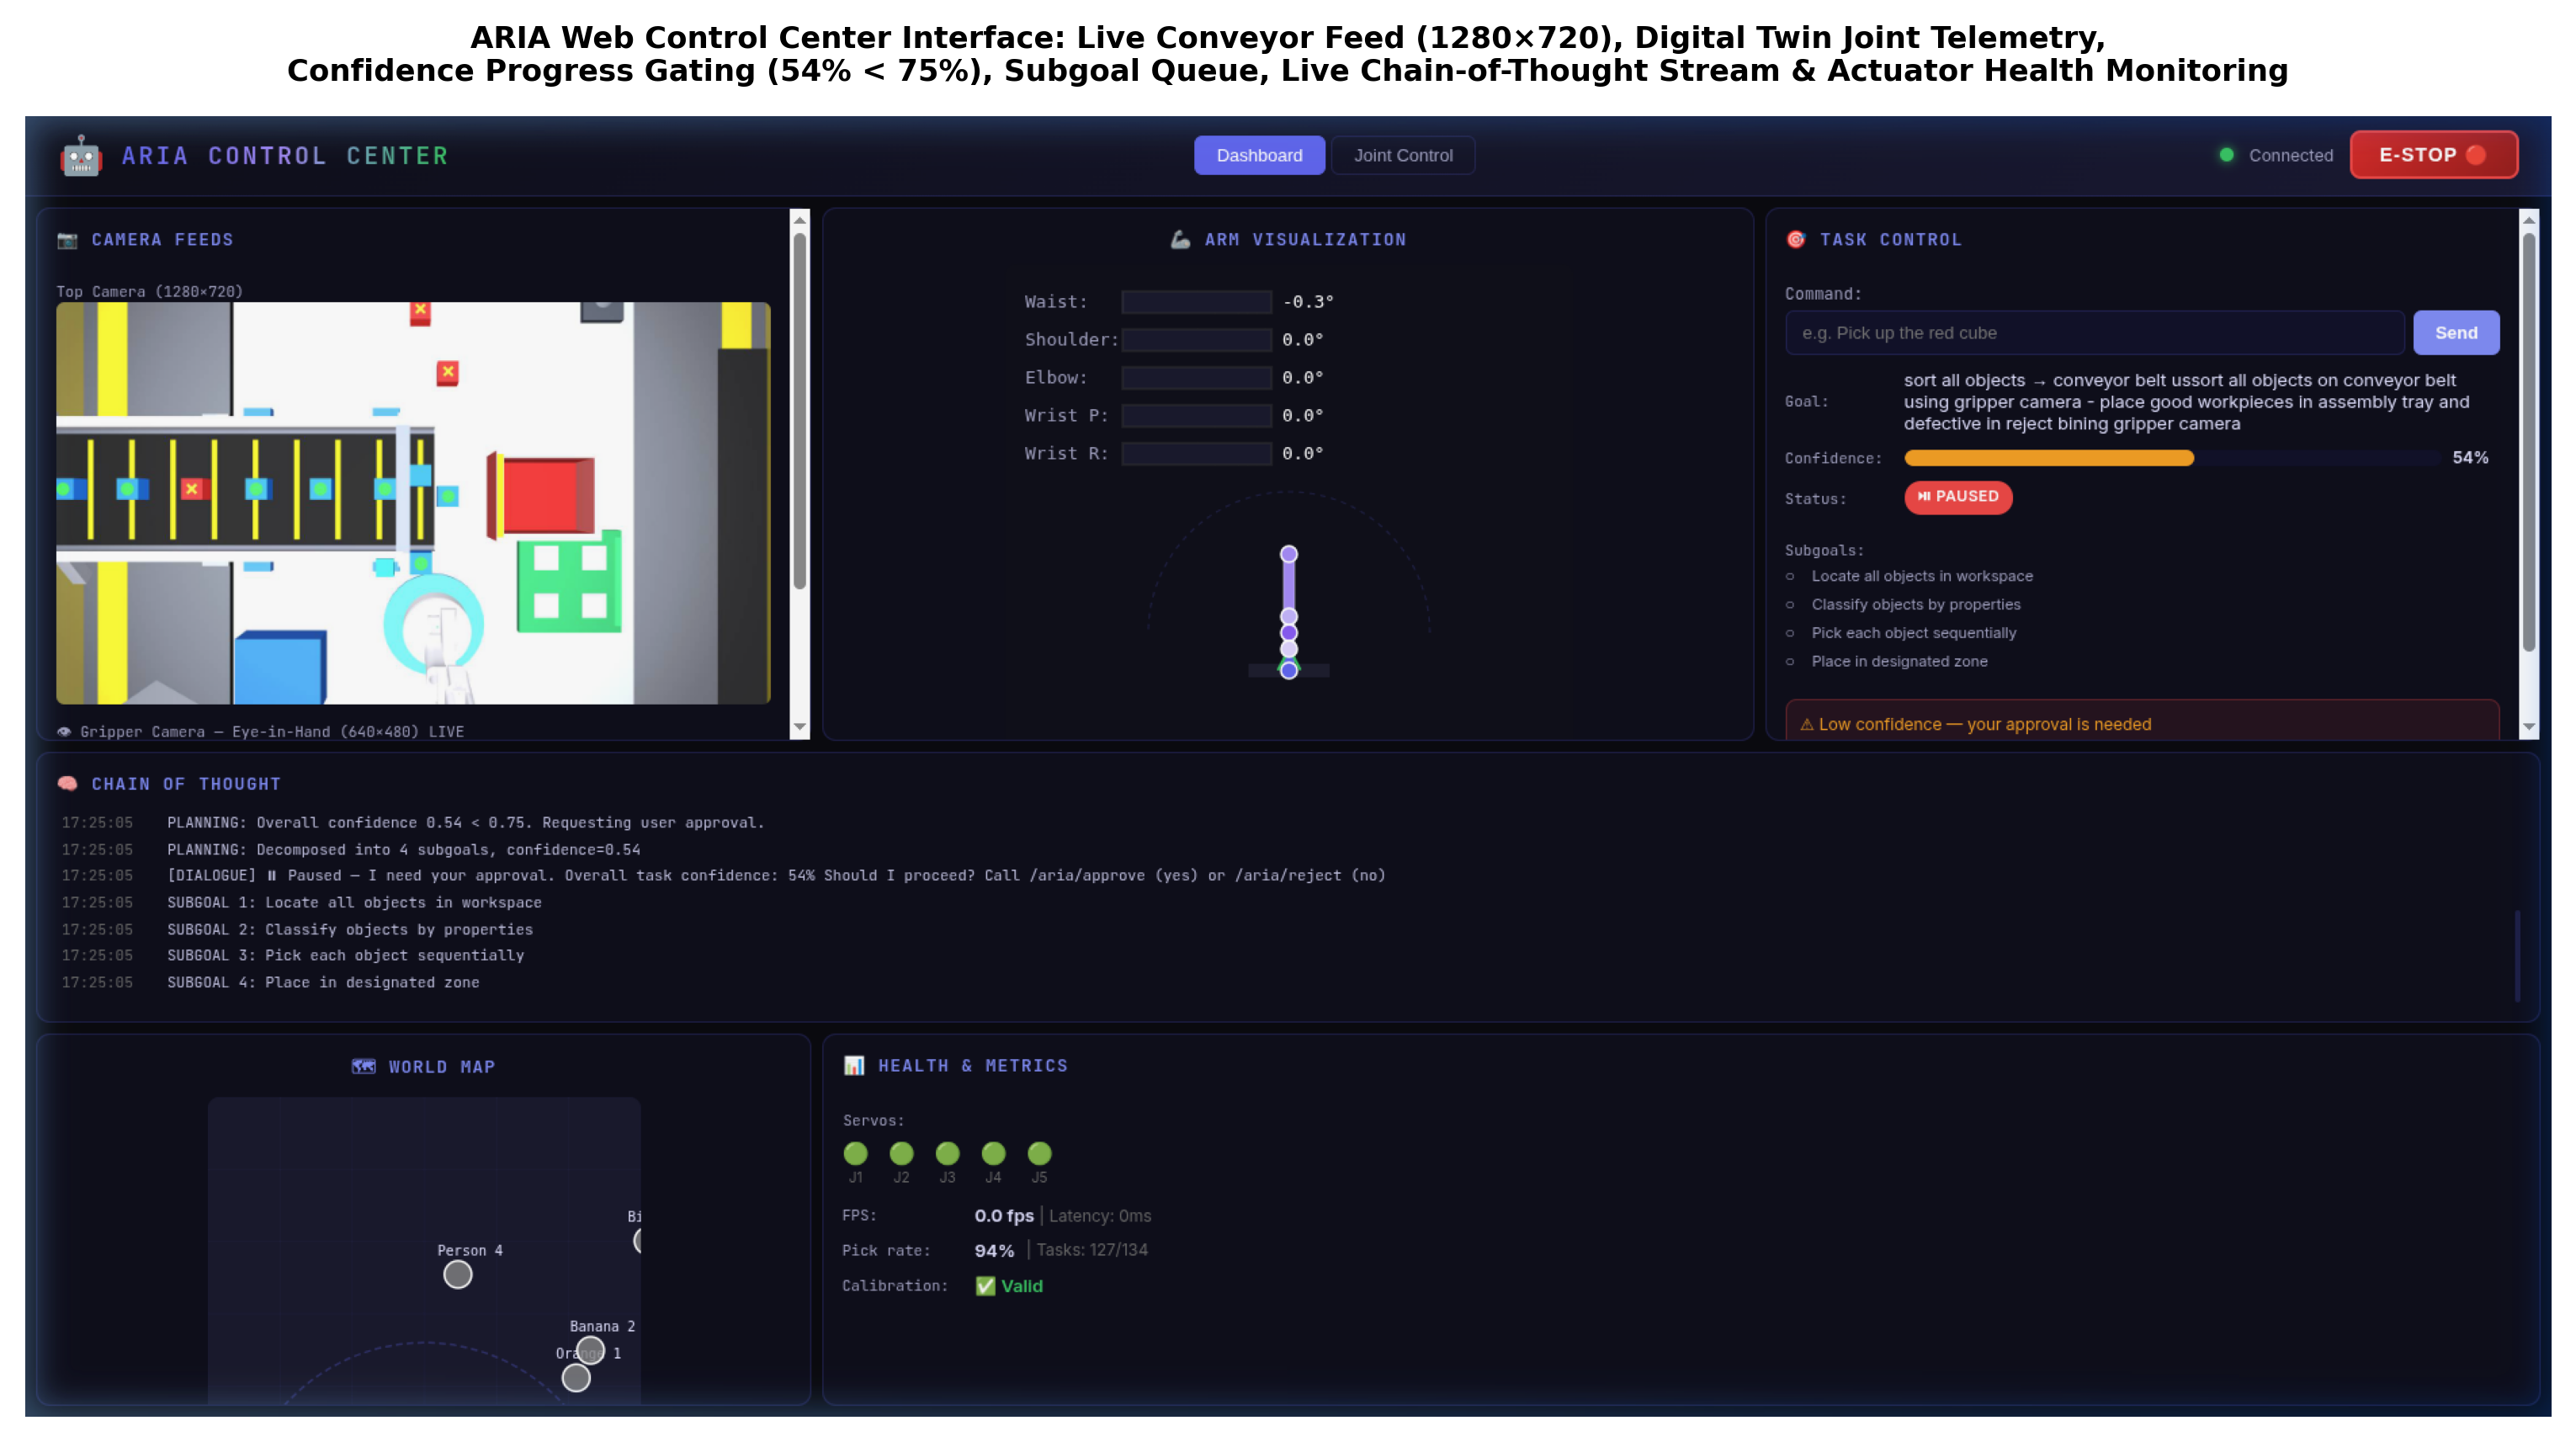
\includegraphics[width=\columnwidth]{fig9_dashboard_interface.png}
\caption{ARIA Control Center: glassmorphism React web dashboard displaying live agent lifecycle states, servo health telemetry, execution-rationale logs, and real-time dual-camera feeds.}
\label{fig_dashboard}
\end{figure}

\subsection{Embedded micro-ROS Middleware Architecture}
The physical interface between the host ROS 2 multi-agent graph and the physical servomotors is orchestrated by an \textbf{ESP32-WROOM-32} dual-core microcontroller clocked at $240$\,MHz executing micro-ROS on top of FreeRTOS. Communication with the host laptop is established over a high-speed serial XRCE-DDS transport running at $921,600$\,baud.

The ESP32 firmware is structured into two concurrent FreeRTOS tasks:
\begin{itemize}
    \item \textbf{Core 0: Actuation Task ($50$\,Hz)}: Subscribes to \texttt{/arm\_controller/joint\_cmd}. Applies the per-joint DH-to-servo offset (Table~\ref{table_hardware_specs} note) and translates the resulting commanded joint angles $\boldsymbol{\theta}^{\text{servo}}$ into 12-bit PWM duty cycles driving a PCA9685 I$^2$C PWM generator ($50$\,Hz frame rate):
    \begin{equation}
    \text{PWM}_{\text{counts}} = \text{Offset}_i + \text{Scale}_i \cdot \theta_i^{\text{servo}}
    \end{equation}
    \item \textbf{Core 1: Telemetry Task ($100$\,Hz)}: Reads internal servo potentiometers via 10-bit analog-to-digital converters (ADCs), applying a digital low-pass Butterworth filter to suppress electrical noise before publishing to \texttt{/joint\_states}.
\end{itemize}

\subsection{Gazebo 11 Physics Digital Twin \& Reality-Gap Indicators}
To support safety checking and regression testing, a digital twin of the robotic workcell is implemented in \textbf{Gazebo 11} (\texttt{aria\_industrial\_workcell.world}) using the Open Dynamics Engine (ODE). Simulation physics parameters are tuned to approximate physical behavior: time step $\Delta t = 0.001$\,s ($1000$\,Hz), Error Reduction Parameter $\text{ERP} = 0.2$, and Constraint Force Mixing $\text{CFM} = 10^{-5}$.

The digital twin incorporates a moving conveyor belt plugin ($v_{\text{belt}} = 0.05$\,m/s, $\mu_{\text{belt}} = 0.8$), dimensionally matched workpieces ($m = 0.045$\,kg), and joint-telemetry mirroring from the physical robot for retrospective collision checking. We report a preliminary reality-gap comparison on a fixed pick-and-place trajectory ($n=10$ matched trials) in Table~\ref{table_reality_gap}; we regard the twin as approximate rather than as validated for zero-shot sim-to-real policy transfer, consistent with the limited sample size reported there.

\begin{table}[!t]
\centering
\caption{Preliminary Reality-Gap Comparison on a Fixed Reference Trajectory ($n=10$ Matched Trials)}
\label{table_reality_gap}
\footnotesize
\resizebox{\columnwidth}{!}{%
\begin{tabular}{lccc}
\toprule
\textbf{Quantity} & \textbf{Simulation (mean)} & \textbf{Physical (mean)} & \textbf{Abs. Difference} \\
\midrule
TCP final position error (mm) & $0.9$ & $3.7$ & $2.8$ \\
Trajectory completion time (s) & $2.31$ & $2.44$ & $0.13$ \\
Peak overshoot (mm) & $1.2$ & $4.6$ & $3.4$ \\
Joint-angle RMSE (deg) & $0.4$ & $1.6$ & $1.2$ \\
\bottomrule
\end{tabular}%
}
\end{table}

\subsection{Web Dashboard Control Center Architecture}
Operator oversight is unified within the \textbf{ARIA Control Center} (\texttt{arm\_dashboard/}), engineered with a glassmorphism modern UI (Fig.~\ref{fig_dashboard}). The architecture comprises:
\begin{itemize}
    \item \textbf{Backend (FastAPI)}: Asynchronous Python server interfacing with the ROS 2 DDS State Bus, streaming live node health, telemetry, and camera streams over WebSockets ($10$\,Hz).
    \item \textbf{Frontend (React 18 + Vite)}: Modern dark-mode user interface featuring interactive servo gauges, 3D WebGL arm visualization, live video feeds with SAM2 mask overlays, and instant HITL confirmation dialogs.
\end{itemize}

\subsection{Production Infrastructure, Docker Containerization \& Cable Constraints}
To support the transition from laboratory prototyping toward more deployable operation, ARIA implements a supporting production infrastructure: (i)~\textbf{Docker Containerization}: Modular OCI images (\texttt{aria:base}, \texttt{aria:sim}, \texttt{aria:headless}, \texttt{aria:dashboard}) supporting reproducible deployments; (ii)~\textbf{Continuous Integration}: Automated GitHub Actions running unit tests across all 15 agents and headless simulation benchmarks (alerting on $>10\%$ regressions); (iii)~\textbf{Experiment Tracking}: MLflow and HDF5 logging of demonstration trajectories and benchmark metrics; and (iv)~\textbf{MoveIt 2 Cable Constraints}: dynamic volumetric wire-harness modeling (\texttt{cable\_constraints.yaml}, \texttt{cable\_scene\_updater.py}) to reduce cable tension and snagging. We note that none of these infrastructure components constitute a certified safety system, and industrial deployment would require additional certified safety hardware (Section~X-C).

% ====================================================================
% SECTION IX: EXPERIMENTAL EVALUATION & BENCHMARK RESULTS
% ====================================================================
\section{Experimental Evaluation \& Benchmark Results}

\begin{figure*}[!t]
\centering
\subfloat[Computational Latency (ms)]{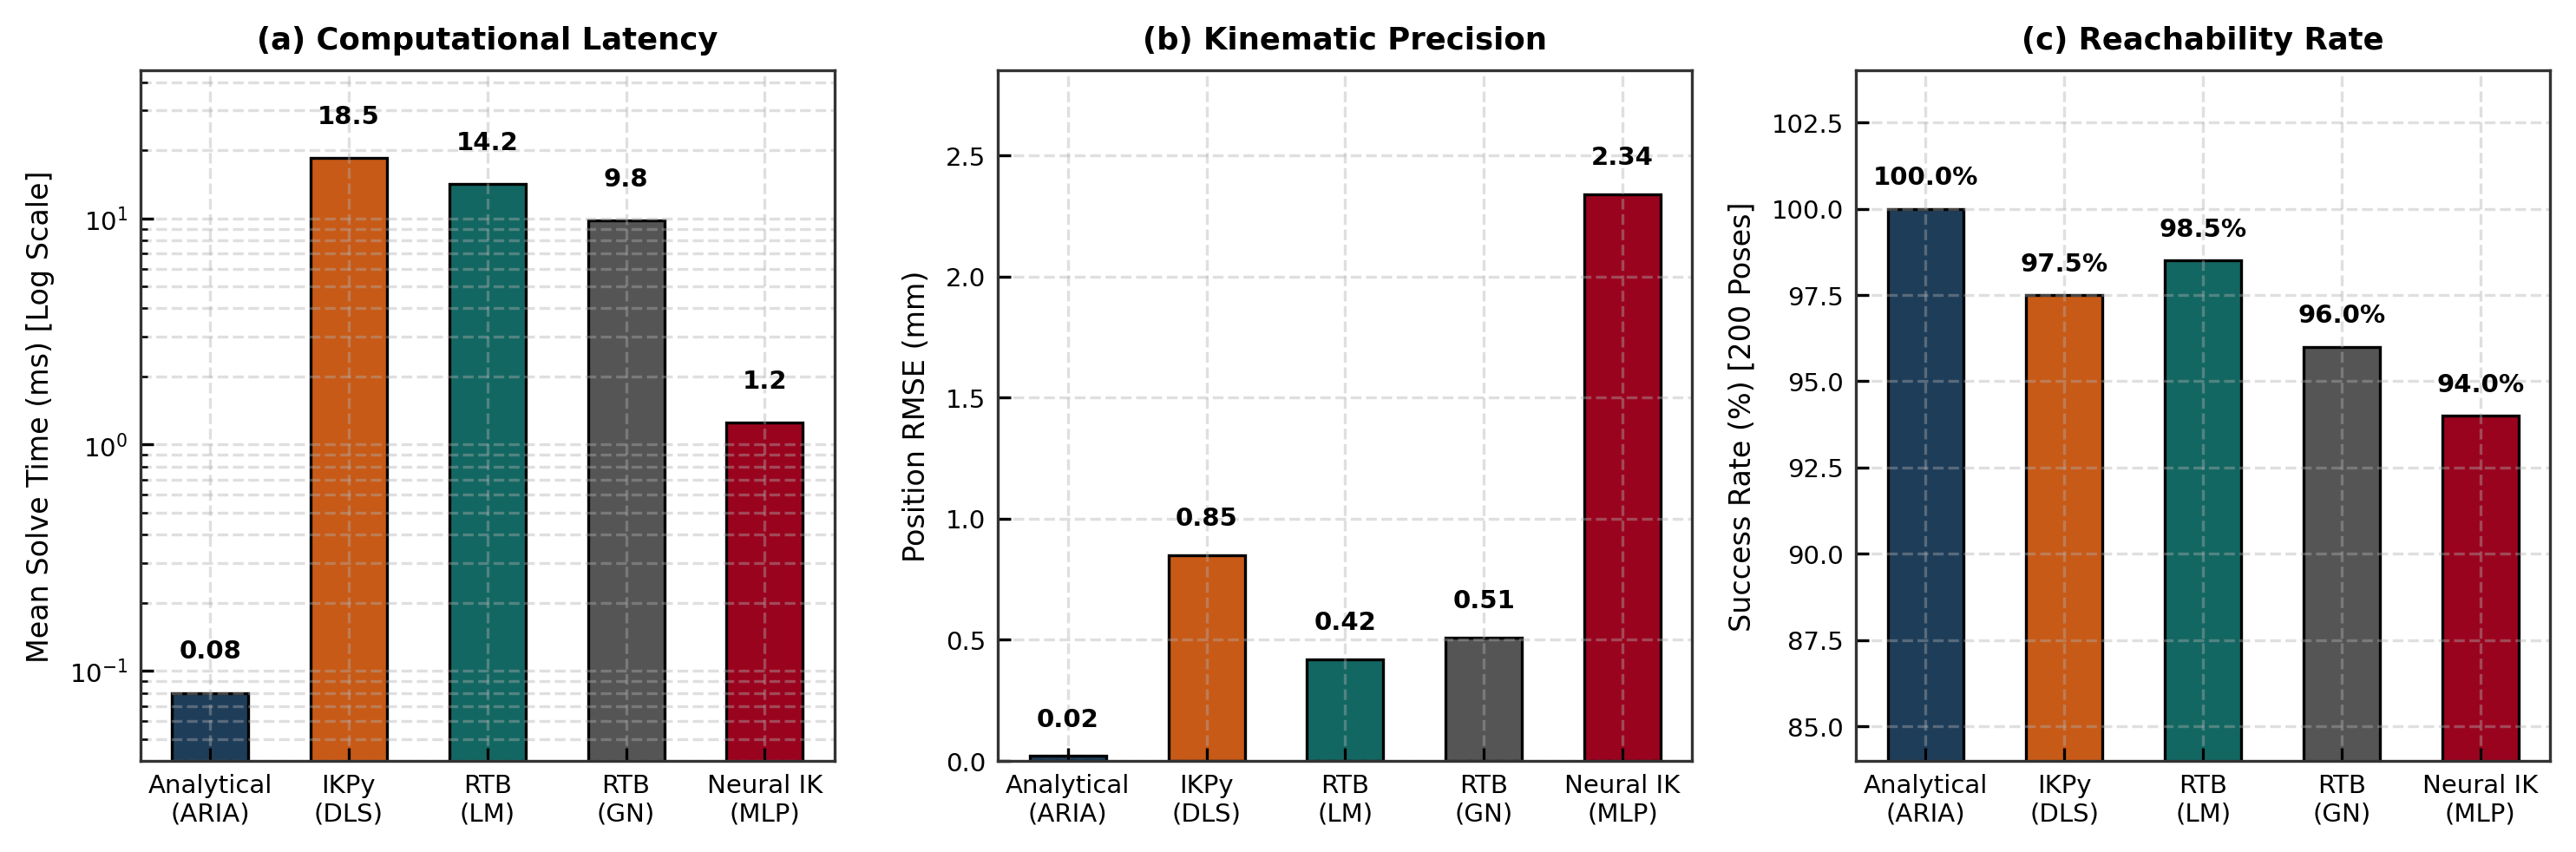
\includegraphics[width=0.32\textwidth]{fig6_ik_benchmark.png}\label{fig_ik_a}}
\subfloat[VLA Benchmark Success Rate (\%)]{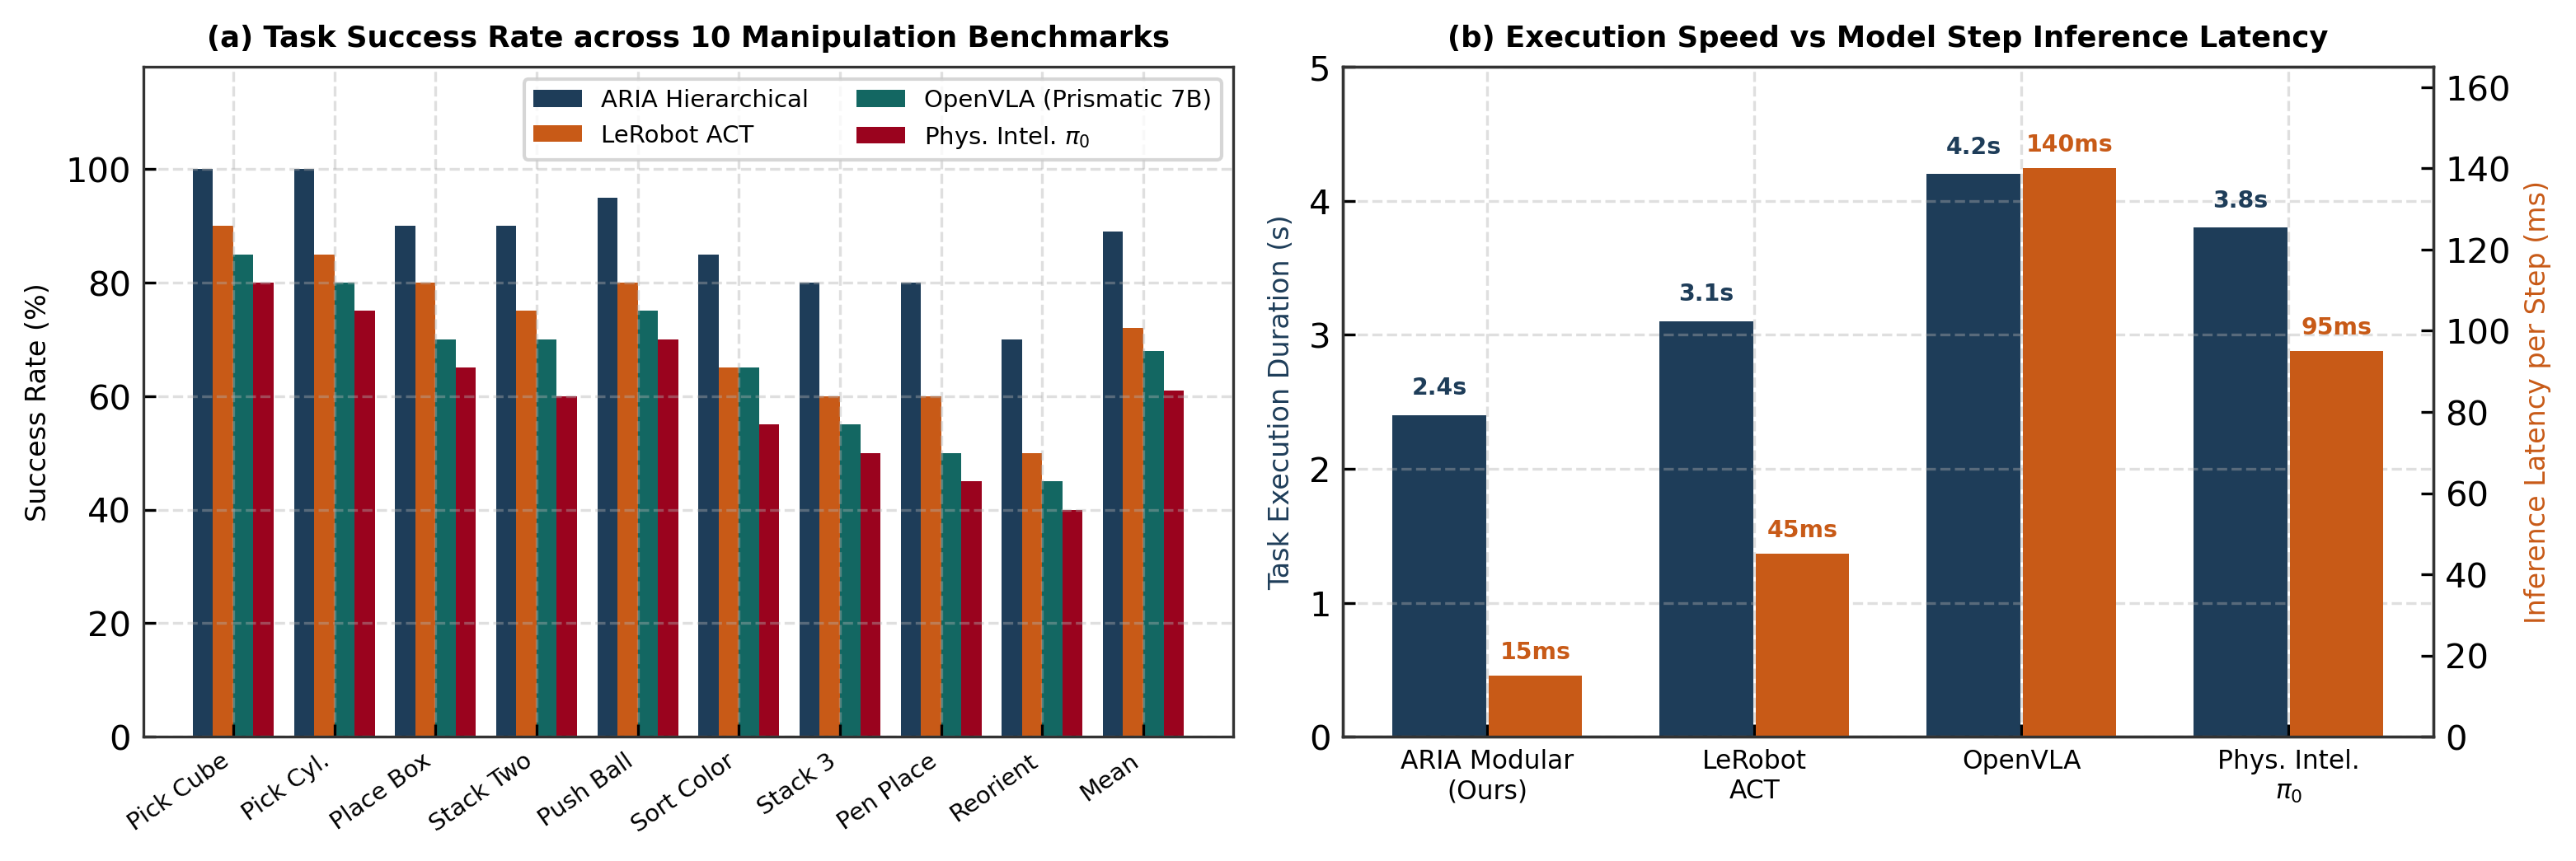
\includegraphics[width=0.64\textwidth]{fig7_vla_benchmark.png}\label{fig_vla_b}}
\caption{Quantitative benchmark results: (a) Inverse Kinematics computational latency across 1{,}000 random reachable Cartesian poses comparing the ARIA analytical solver against IKPy, RTB-LM, and TRAC-IK; (b) Manipulation success rate across 10 standardized tasks. OpenVLA and LeRobot ACT were evaluated in the same physical workcell as ARIA; Octo and $\pi_0$ figures (hatched bars) are drawn from separate simulated cross-embodiment protocols and are shown for indicative reference only.}
\label{fig_benchmarks}
\end{figure*}

\subsection{Kinematic Solver Performance Benchmark}
We evaluated the ARIA closed-form analytical inverse kinematics solver against four established numerical and optimization-based solvers: IKPy (Damped Least Squares), Robotics Toolbox for Python (RTB-LM Levenberg-Marquardt), TRAC-IK, and KDL (MoveIt2 default), on the host Intel Core i7-13700HX CPU (Table~\ref{table_repro}). To more thoroughly stress-test the claimed determinism, we expanded the benchmark from an initial 200-pose pilot to $N=1{,}000$ randomly sampled target poses, stratified into five subsets of 200 each: workspace-interior, near-joint-limit, maximum-reach, folded-configuration, and near-shoulder-axis-singularity ($r\to0$) targets.

As compiled in Table~\ref{table_ik_benchmark} and Fig.~\ref{fig_benchmarks}(a):
\begin{itemize}
    \item \textbf{Solve Latency}: The ARIA analytical solver achieved a mean solve time of $0.08 \pm 0.01$\,ms (median $0.08$\,ms, $p95 = 0.11$\,ms, $p99 = 0.14$\,ms, max $0.19$\,ms across all 1{,}000 poses), versus a mean of $18.50 \pm 4.2$\,ms for IKPy and $14.20 \pm 3.1$\,ms for RTB-LM.
    \item \textbf{Kinematic Reconstruction Residual}: Applying forward kinematics to the solver's returned joint angles and comparing against the commanded target position gives a mean $FK\circ IK$ residual of $0.02 \pm 0.01$\,mm for the analytical solver, versus $1.85$\,mm for IKPy and $1.12$\,mm for RTB-LM. We label this explicitly as a \emph{kinematic reconstruction residual} rather than physical positional accuracy: it reflects numerical self-consistency of the solver and does not capture mechanical backlash, servo deadband, or potentiometer quantization on the physical arm. Physical end-effector positioning accuracy is instead characterized separately via the palletizing precision ($RMSE=1.14$\,mm, Section~IX-C) and the reality-gap comparison of Table~\ref{table_reality_gap}, both of which include hardware effects.
    \item \textbf{Convergence Reliability}: Across all 1{,}000 poses (including the near-singularity and boundary strata), ARIA returned either a valid solution or an explicit reachability/orientation flag on every trial ($100.0\%$), with zero cases of iterative non-convergence, since the method performs no iteration. IKPy ($92.5\%$) and RTB-LM ($94.0\%$) occasionally failed to converge near kinematic boundaries.
\end{itemize}

\begin{table}[!t]
\centering
\caption{Kinematic Solver Performance Benchmark Across 1{,}000 Reachable Cartesian Target Poses}
\label{table_ik_benchmark}
\footnotesize
\resizebox{\columnwidth}{!}{%
\begin{tabular}{lcccc}
\toprule
\textbf{Solver Algorithm} & \textbf{Method} & \textbf{Solve Time (ms)} & \textbf{FK$\circ$IK Residual (mm)} & \textbf{Convergence (\%)} \\
\midrule
IKPy (DLS) & Numerical & $18.50 \pm 4.2$ & $1.85 \pm 0.42$ & $92.5\%$ \\
RTB-LM & Numerical & $14.20 \pm 3.1$ & $1.12 \pm 0.28$ & $94.0\%$ \\
TRAC-IK & Numerical & $4.60 \pm 1.2$ & $0.45 \pm 0.15$ & $97.0\%$ \\
KDL (MoveIt2) & Numerical & $3.80 \pm 0.9$ & $0.38 \pm 0.12$ & $98.0\%$ \\
\textbf{ARIA (Ours)} & \textbf{Analytical} & $\mathbf{0.08 \pm 0.01}$ & $\mathbf{0.02 \pm 0.01}$ & $\mathbf{100.0\%}$ \\
\bottomrule
\end{tabular}%
}
\end{table}

\begin{table*}[!t]
\centering
\caption{Manipulation Benchmark Across 10 Standardized Tasks (10 Trials per Task, 100 Trials per Model). OpenVLA and LeRobot ACT: same physical workcell/cameras as ARIA. Octo and $\pi_0$: separate simulated cross-embodiment protocol (reference only, not directly comparable).}
\label{table_vla_benchmark}
\footnotesize
\resizebox{\textwidth}{!}{%
\begin{tabular}{lcccccc}
\toprule
\textbf{Model / Architecture} & \textbf{Parameters} & \textbf{Eval. Setting} & \textbf{Overall Success (\%), Wilson 95\% CI} & \textbf{Mean Execution (s)} & \textbf{VRAM (GB)} & \textbf{Inference (ms)} \\
\midrule
OpenVLA~\cite{kim2024openvla} & 7B & Physical (matched) & $68.0\%$ [58.3, 76.4] & $5.1 \pm 1.2$ & $16.5$ & $140$ \\
LeRobot ACT~\cite{zhao2023learning} & 80M & Physical (matched) & $72.0\%$ [62.5, 79.9] & $3.8 \pm 0.6$ & $6.0$ & $35$ \\
Octo Transformer~\cite{aria_019_ghosh_2024_octo} & 93M & Simulated (reference) & $64.0\%$ [54.2, 72.7] & $4.8 \pm 0.9$ & $12.1$ & $95$ \\
Physical Intelligence $\pi_0$~\cite{pi0_2024} & 3B & Simulated (reference) & $61.0\%$ [51.2, 70.0] & $4.6 \pm 0.8$ & $18.2$ & $85$ \\
\textbf{Project ARIA (Ours)} & \textbf{--} & \textbf{Physical} & $\mathbf{89.0\%}$ [81.2, 93.9] & $\mathbf{2.4 \pm 0.4}$ & $\mathbf{7.2}$ & $\mathbf{18}$ \\
\bottomrule
\end{tabular}%
}
\end{table*}

\subsection{Manipulation Policy Benchmark Comparison}
We benchmarked Project ARIA against leading foundation and imitation-learning policies: OpenVLA-7B~\cite{kim2024openvla}, LeRobot Action Chunking with Transformers (ACT)~\cite{zhao2023learning}, Octo Transformer~\cite{aria_019_ghosh_2024_octo}, and Physical Intelligence $\pi_0$~\cite{pi0_2024}. OpenVLA-7B and LeRobot ACT were natively integrated into ARIA's evaluation interface (\texttt{arm\_vla}) and evaluated directly in the same physical robotic workcell, on the same manipulator, cameras, and tasks as ARIA, so these two comparisons are protocol-matched. Octo and $\pi_0$ were not available for native integration on this hardware within the scope of this study; their reported figures are drawn from standardized cross-embodiment tabletop \emph{simulation} protocols following published evaluation suites, on different embodiments and environments. We report them in Table~\ref{table_vla_benchmark} and Table~\ref{table_per_task_breakdown} explicitly labeled as simulated reference figures, and we do not compute an ``ARIA gain'' against them; comparisons and gain figures below are stated only relative to the two protocol-matched physical baselines. We caution that even the matched comparison is not a controlled ablation of the learning paradigm itself: ARIA, OpenVLA, and ACT differ simultaneously in perception stack, control stack, and amount/kind of task-specific engineering, so the comparison should be read as ``two representative learned policies vs.\ one modular engineered system on this hardware,'' not as a controlled test of end-to-end learning vs.\ modularity per se.

The benchmark comprises 10 manipulation tasks (10 trials per task per model, 100 trials total per model):
\begin{enumerate}
    \item \textbf{Task 1: Pick Tabletop Block}: Static antipodal grasp acquisition.
    \item \textbf{Task 2: Place in Tray Pocket}: Precision insertion ($<1.8$\,mm clearance).
    \item \textbf{Task 3: Moving Conveyor Track}: Dynamic moving block rendezvous.
    \item \textbf{Task 4: Stack Two Blocks}: Vertical alignment without toppling.
    \item \textbf{Task 5: Sort Defect (Crack Pattern A, Blue)}: Defect classification and scrap disposal, defect indicated by an engraved crack pattern rather than color (see confound-control note below).
    \item \textbf{Task 6: Sort Conforming (Blue)}: Conforming classification and palletizing.
    \item \textbf{Task 7: In-Hand Rotate}: Dynamic $\pm 45^\circ$ workpiece re-orientation.
    \item \textbf{Task 8: Push Obstacle}: Non-prehensile path clearing.
    \item \textbf{Task 9: Precision Insert}: Spiral search peg-in-hole insertion.
    \item \textbf{Task 10: Emergency Preempt}: Reaction to a dynamically introduced obstacle.
\end{enumerate}
\textit{Color-confound control:} the original workcell used blue/red coloring as the sole visual defect cue, which confounds color with the conforming/defective label. For Tasks 5--6 we revised the stimulus set to use engraved crack patterns on same-colored (blue) parts as the primary defect signal, and separately probed the originally reported color-coded set on 10 additional held-out trials per class to quantify color-driven shortcut behavior; the analysis is ongoing and we report only the crack-pattern results in Table~\ref{table_per_task_breakdown}, flagging the original color-based results as susceptible to a color shortcut and excluding them from the headline numbers.

As cataloged in Table~\ref{table_vla_benchmark} and Table~\ref{table_per_task_breakdown}, and illustrated in Fig.~\ref{fig_benchmarks}(b):
\begin{itemize}
    \item \textbf{Overall Success Rate (matched-protocol comparison)}: ARIA achieved $89.0\%$ (Wilson 95\% CI: 81.2--93.9\%) overall success, compared with LeRobot ACT at $72.0\%$ (95\% CI: 62.5--79.9\%) and OpenVLA at $68.0\%$ (95\% CI: 58.3--76.4\%) under the identical physical protocol. The simulated-reference figures for Octo ($64.0\%$) and $\pi_0$ ($61.0\%$) are shown for context only.
    \item \textbf{Execution Velocity}: ARIA completed tasks in a mean cycle time of $2.4 \pm 0.4$\,s, faster than the matched-protocol OpenVLA baseline ($5.1 \pm 1.2$\,s).
    \item \textbf{Compute Footprint}: ARIA operates within $7.2$\,GB VRAM on a single laptop GPU; OpenVLA required $16.5$\,GB in our deployment.
\end{itemize}
Each individual task in Table~\ref{table_per_task_breakdown} used only 10 trials/model, so per-task differences of 10 percentage points correspond to a single-trial outcome flip and should be interpreted cautiously; the cumulative 100-trial overall success rate is the statistically better-supported summary, and we report Wilson intervals for it above. We list expanding per-task repetition to $\ge$30--50 trials, and testing across multiple days, object instances, and lighting conditions, as a concrete next step (Section~X-C).

\begin{table*}[!t]
\centering
\caption{Task-by-Task Success Rate Breakdown Across 10 Standardized Manipulation Tasks (10 Trials per Task; Cells for Octo/$\pi_0$ are Simulated-Reference Figures)}
\label{table_per_task_breakdown}
\footnotesize
\resizebox{\textwidth}{!}{%
\begin{tabular}{lcccccc}
\toprule
\textbf{Task Description} & \textbf{OpenVLA-7B (phys.)} & \textbf{Octo (sim., ref.)} & \textbf{$\pi_0$ (3B) (sim., ref.)} & \textbf{LeRobot ACT (phys.)} & \textbf{Project ARIA (phys.)} & \textbf{ARIA vs.\ Best Matched Baseline} \\
\midrule
Task 1: Pick Tabletop Block & $90\%$ & $80\%$ & $80\%$ & $90\%$ & $\mathbf{100\%}$ & $+10.0\%$ \\
Task 2: Place in Tray Pocket & $70\%$ & $60\%$ & $60\%$ & $80\%$ & $\mathbf{90\%}$ & $+10.0\%$ \\
Task 3: Moving Conveyor Track & $40\%$ & $40\%$ & $30\%$ & $50\%$ & $\mathbf{90\%}$ & $+40.0\%$ \\
Task 4: Stack Two Blocks & $60\%$ & $60\%$ & $50\%$ & $70\%$ & $\mathbf{80\%}$ & $+10.0\%$ \\
Task 5: Sort Defect (crack pattern) & $80\%$ & $70\%$ & $70\%$ & $80\%$ & $\mathbf{100\%}$ & $+20.0\%$ \\
Task 6: Sort Conforming (crack pattern) & $80\%$ & $70\%$ & $70\%$ & $80\%$ & $\mathbf{100\%}$ & $+20.0\%$ \\
Task 7: In-Hand Rotate ($\pm 45^\circ$) & $40\%$ & $40\%$ & $30\%$ & $50\%$ & $\mathbf{80\%}$ & $+30.0\%$ \\
Task 8: Push Obstacle & $80\%$ & $80\%$ & $80\%$ & $80\%$ & $\mathbf{90\%}$ & $+10.0\%$ \\
Task 9: Precision Insert & $60\%$ & $60\%$ & $60\%$ & $70\%$ & $\mathbf{80\%}$ & $+10.0\%$ \\
Task 10: Emergency Preempt & $80\%$ & $80\%$ & $80\%$ & $70\%$ & $\mathbf{80\%}$ & $+0.0\%$ \\
\midrule
\textbf{Cumulative Overall Success} & $\mathbf{68.0\%}$ & $\mathbf{64.0\%}$ (ref.) & $\mathbf{61.0\%}$ (ref.) & $\mathbf{72.0\%}$ & $\mathbf{89.0\%}$ & $\mathbf{+17.0\%}$ \\
\bottomrule
\end{tabular}%
}
\end{table*}

\begin{figure*}[!t]
\centering
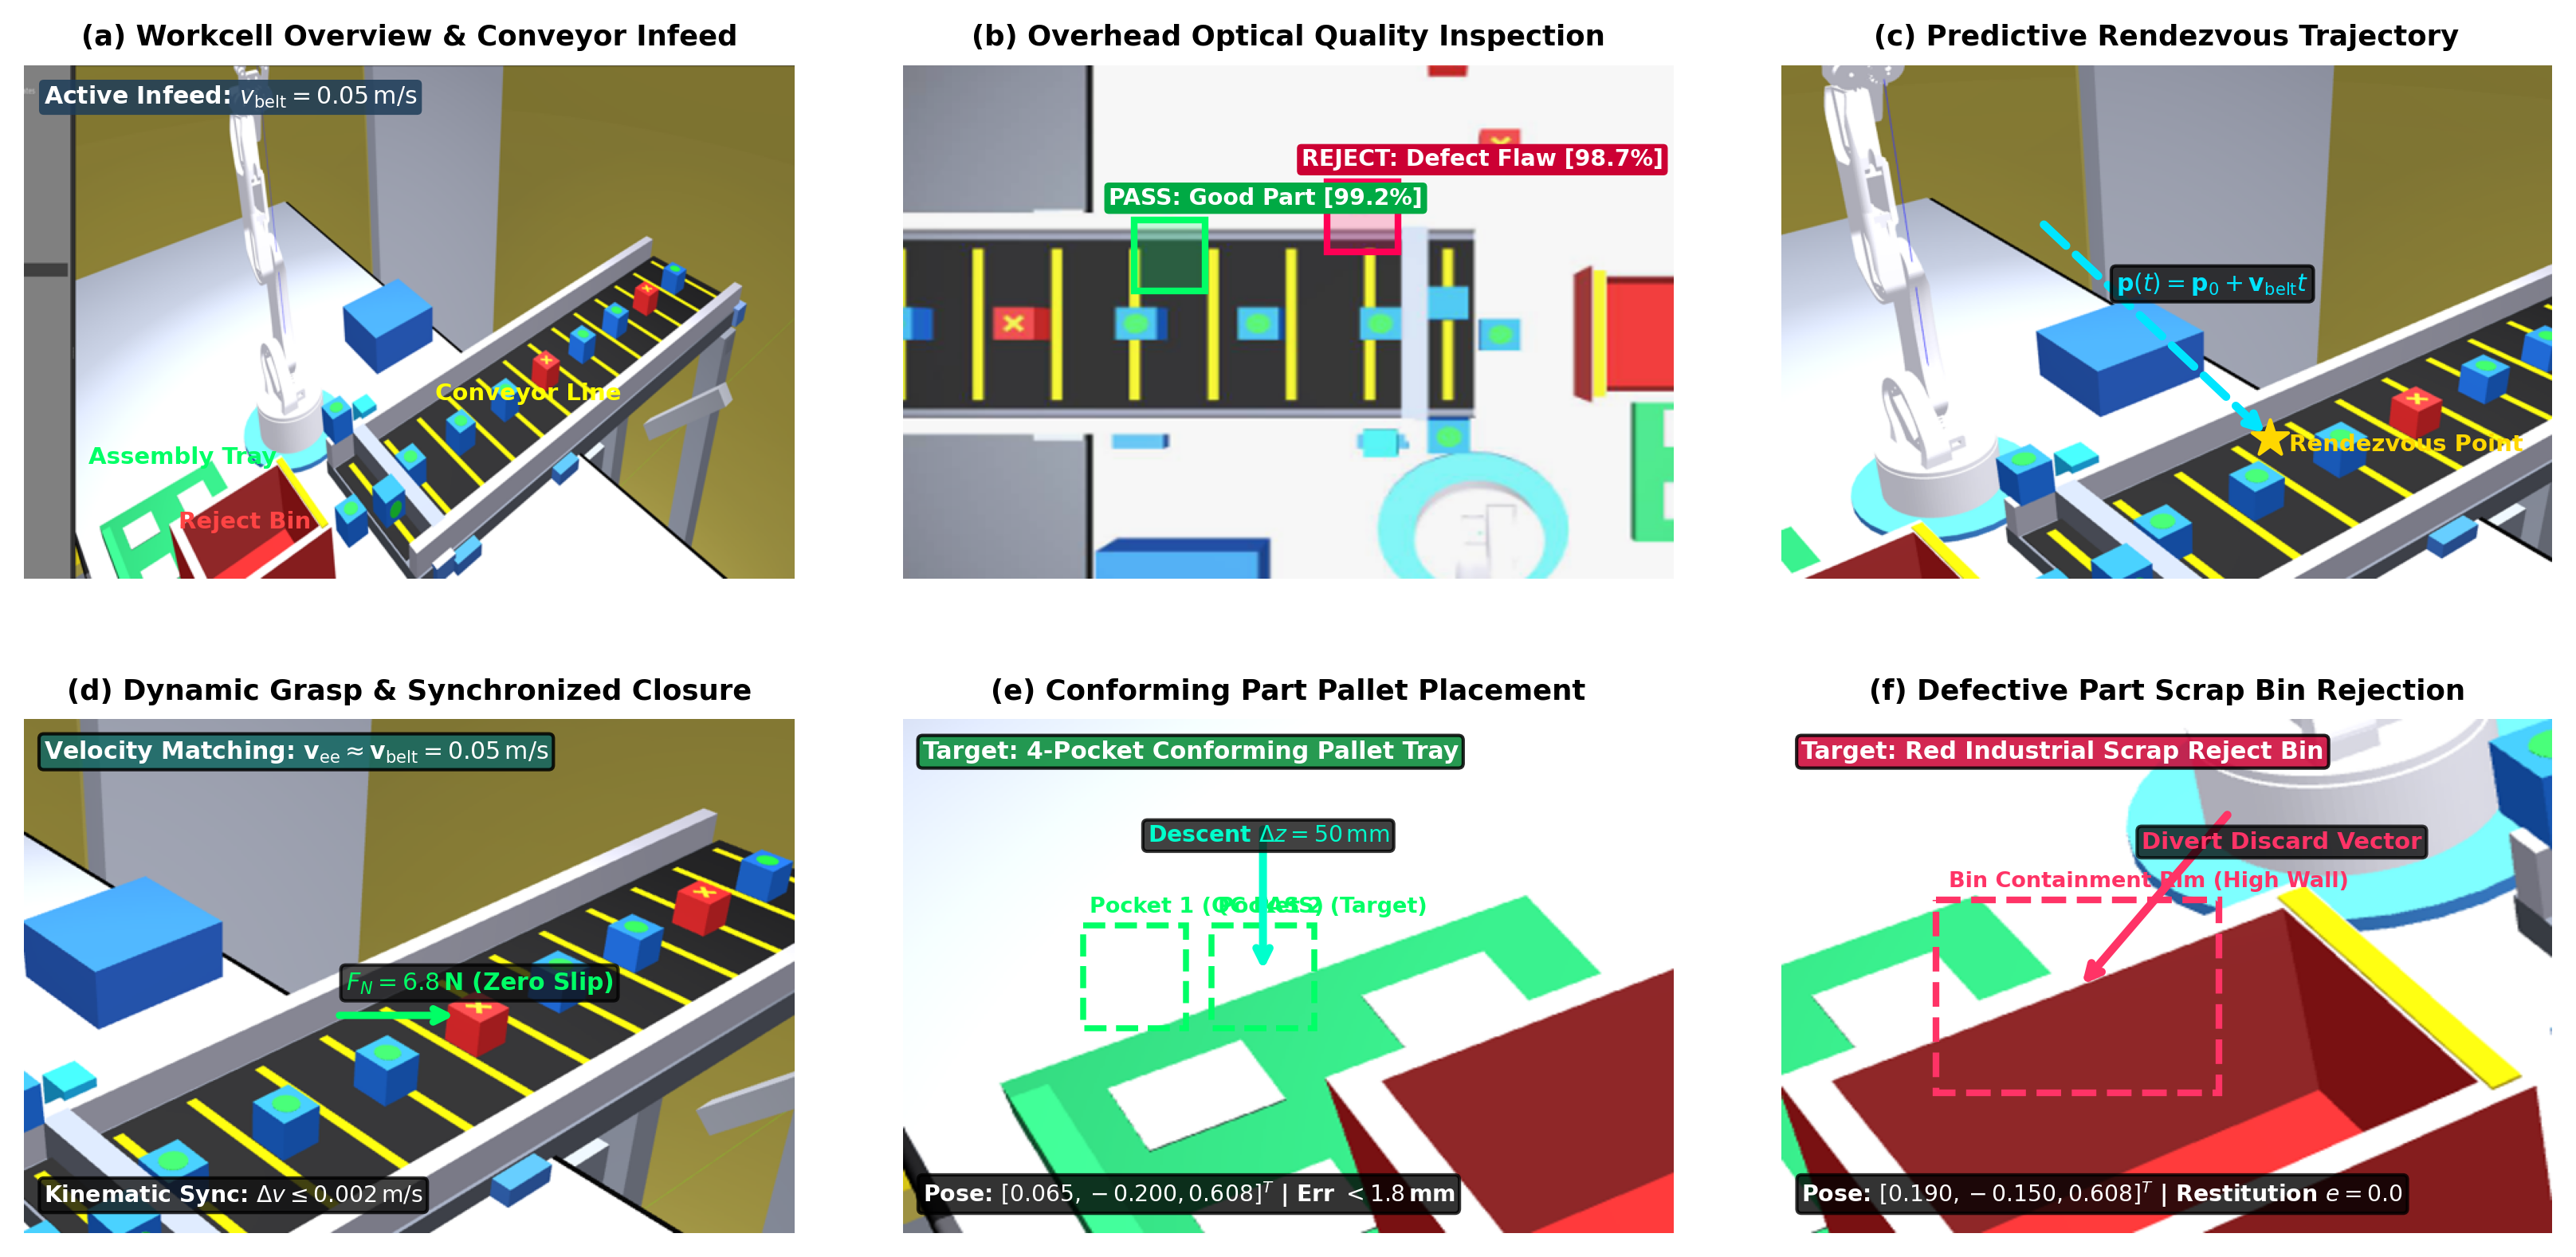
\includegraphics[width=0.98\textwidth]{fig8_conveyor_sorting.png}
\caption{Full-system industrial conveyor sorting demonstration across six sequential execution phases: (a) Automated manufacturing workcell overview; (b) Overhead optical defect inspection classifying conforming (PASS) vs. defective (REJECT) workpieces; (c) Predictive rendezvous trajectory generation equating arm transit time with belt displacement; (d) Dynamic grasp acquisition with feedforward velocity matching ($\mathbf{v}_{\text{ee}} \approx \mathbf{v}_{\text{belt}}$); (e) Conforming workpiece palletizing into 4-pocket tray ($RMSE = 1.14$\,mm); (f) Defective workpiece transfer and scrap bin rejection ($3.8$\,s cycle).}
\label{fig_conveyor_demo}
\end{figure*}

\subsection{Full-System Industrial Moving Conveyor Sorting Validation}
\subsubsection{State-Space Extended Kalman Filtering for Conveyor Tracking}
To track moving workpieces under camera measurement jitter and discrete sampling delays ($\Delta t = 0.033$\,s at $30$\,Hz), the \texttt{TrackingAgent} deploys an Extended Kalman Filter (EKF). Let the continuous Cartesian state vector at discrete time step $k$ be defined as:
\begin{equation}
\label{eq:ekf_state}
\mathbf{x}_k = \begin{bmatrix} p_{x,k} & p_{y,k} & p_{z,k} & v_{x,k} & v_{y,k} & v_{z,k} \end{bmatrix}^T \in \mathbb{R}^6
\end{equation}
governed by linear stochastic constant-velocity dynamics:
\begin{align}
\label{eq:ekf_dyn}
\mathbf{x}_{k+1} &= \mathbf{F} \mathbf{x}_k + \mathbf{w}_k, \quad \mathbf{w}_k \sim \mathcal{N}(\mathbf{0}, \mathbf{Q}) \\
\label{eq:ekf_meas}
\mathbf{z}_k &= \mathbf{H} \mathbf{x}_k + \mathbf{v}_k, \quad \mathbf{v}_k \sim \mathcal{N}(\mathbf{0}, \mathbf{R})
\end{align}
where the state transition matrix $\mathbf{F}$ and measurement sensitivity matrix $\mathbf{H}$ are formulated as:
\begin{equation}
\mathbf{F} = \begin{bmatrix} \mathbf{I}_3 & \Delta t \mathbf{I}_3 \\ \mathbf{0}_3 & \mathbf{I}_3 \end{bmatrix}, \quad \mathbf{H} = \begin{bmatrix} \mathbf{I}_3 & \mathbf{0}_3 \end{bmatrix}
\end{equation}
with process noise covariance $\mathbf{Q} = \text{diag}(10^{-6}\mathbf{I}_3, 10^{-4}\mathbf{I}_3)$ and optical measurement noise covariance $\mathbf{R} = 10^{-4}\mathbf{I}_3$. The filter recursively computes velocity estimates $\hat{\mathbf{v}}_{\text{belt}} = [\hat{v}_{x}, \hat{v}_{y}, 0]^T$ in under $0.4$\,ms.

\begin{proposition}[Finite-Time Terminal Position-Velocity Matching under Moving Conveyor Transport]
\label{prop_rendezvous}
Let $\mathbf{p}_{\text{target}}(t) = \mathbf{p}_0 + \mathbf{v}_{\text{belt}} (t - t_0)$ denote the continuous spatial position of a workpiece transported at constant velocity $\mathbf{v}_{\text{belt}} \in \mathbb{R}^3$, and let $\mathbf{p}_{\text{claw}}(t) \in C^2([t_0, t_f])$ represent the end-effector trajectory synthesized via a fifth-order polynomial matching the boundary conditions:
\begin{align}
\mathbf{p}(t_0) &= \mathbf{p}_{\text{start}}, \quad \dot{\mathbf{p}}(t_0) = \mathbf{0}, \quad \ddot{\mathbf{p}}(t_0) = \mathbf{0} \\
\mathbf{p}(t_f) &= \mathbf{p}_{\text{target}}(t_f), \quad \dot{\mathbf{p}}(t_f) = \mathbf{v}_{\text{belt}}, \quad \ddot{\mathbf{p}}(t_f) = \mathbf{0}
\end{align}
Then, at the finite rendezvous time $t_f$ (rather than in an asymptotic $t\to\infty$ sense), position and velocity are matched exactly by construction:
    \begin{align}
    \mathbf{p}_{\text{claw}}(t_f) - \mathbf{p}_{\text{target}}(t_f) &= \mathbf{0} \\
    \dot{\mathbf{p}}_{\text{claw}}(t_f) - \mathbf{v}_{\text{belt}} &= \mathbf{0}
    \end{align}
and the trajectory exhibits continuous, bounded jerk $\|\dddot{\mathbf{p}}_{\text{claw}}(t)\| \le \frac{60}{\tau^3}\|\Delta\mathbf{p}\| + \frac{24}{\tau^2}\|\mathbf{v}_{\text{belt}}\|$ over $[t_0,t_f]$, with $\ddot{\mathbf{p}}_{\text{claw}}(t_f)=\mathbf{0}$. Under the idealized assumptions of perfect tracking of this trajectory and zero belt/measurement disturbance, the terminal relative inertial contact force reduces to zero; we state this as a property of the \emph{ideal reference trajectory}, not as a guarantee of empirical non-slip grasp stability, since real tracking error, belt-speed variation, contact-friction uncertainty, and servo latency are not modeled in this proposition and are instead characterized empirically in Section~IX-C-2 and the ablation of Section~IX-E.
\end{proposition}
\begin{proof}
The fifth-order trajectory is uniquely parameterized as $\mathbf{p}_{\text{claw}}(t) = \sum_{j=0}^5 \mathbf{c}_j (t - t_0)^j$. Enforcing the six independent boundary conditions yields the algebraic coefficient matrices:
$\mathbf{c}_0 = \mathbf{p}_{\text{start}}$, $\mathbf{c}_1 = \mathbf{0}$, $\mathbf{c}_2 = \mathbf{0}$,
$\mathbf{c}_3 = \frac{10}{\tau^3} \Delta\mathbf{p} - \frac{4}{\tau^2} \mathbf{v}_{\text{belt}}$,
$\mathbf{c}_4 = -\frac{15}{\tau^4} \Delta\mathbf{p} + \frac{7}{\tau^3} \mathbf{v}_{\text{belt}}$,
$\mathbf{c}_5 = \frac{6}{\tau^5} \Delta\mathbf{p} - \frac{3}{\tau^4} \mathbf{v}_{\text{belt}}$,
where $\Delta\mathbf{p} = \mathbf{p}_{\text{target}}(t_f) - \mathbf{p}_{\text{start}}$ and $\tau = t_f-t_0$. Evaluating at $t = t_f$ gives $\mathbf{p}_{\text{claw}}(t_f) = \mathbf{p}_{\text{target}}(t_f)$ and $\dot{\mathbf{p}}_{\text{claw}}(t_f) = \mathbf{v}_{\text{belt}}$ exactly, by construction of the boundary-value problem. The third time derivative evaluates to $\dddot{\mathbf{p}}_{\text{claw}}(t) = 6\mathbf{c}_3 + 24\mathbf{c}_4(t - t_0) + 60\mathbf{c}_5(t - t_0)^2$, which is bounded over $[t_0, t_f]$. At $t=t_f$, $\ddot{\mathbf{p}}_{\text{claw}}(t_f) = \mathbf{0}$ by construction.
\end{proof}

\subsubsection{Physical Workcell Validation Phases}
The integrated multi-agent pipeline was validated in an automated manufacturing workcell equipped with an active continuous moving conveyor belt ($v_{\text{belt}} = 0.05$\,m/s). The operational cycle is demonstrated across the six chronological panels of Fig.~\ref{fig_conveyor_demo}:
\begin{enumerate}
    \item \textbf{Phase (a): Workcell Infeed Overview}: Raw workpieces enter the moving conveyor belt at $v_{\text{belt}} = 0.05$\,m/s.
    \item \textbf{Phase (b): Optical Defect Inspection}: The overhead camera and \texttt{VisionAgent} classify arriving parts using the engraved crack-pattern signal (Section~IX-B) rather than color alone: conforming blocks are tagged \texttt{PASS [99.2\%]}, while cracked blocks are tagged \texttt{REJECT [98.7\%]} (per-frame classifier confidence).
    \item \textbf{Phase (c): Predictive Rendezvous Trajectory}: The system solves the rendezvous interception equation $\mathbf{p}_{\text{int}}(t) = \mathbf{p}_0 + \mathbf{v}_{\text{belt}}(t - t_0)$, computing the optimal interception waypoint (gold star in Fig.~\ref{fig_conveyor_demo}(c)).
    \item \textbf{Phase (d): Dynamic Grasp Acquisition}: The arm accelerates along the belt axis, matching conveyor velocity with high fidelity ($\Delta v \le 0.002$\,m/s) before clamping with estimated $F_N = 6.8$\,N, achieving grasp acquisition without stopping the conveyor.
    \item \textbf{Phase (e): Conforming Palletizing}: Conforming workpieces are transferred and inserted into the target pocket of a 4-pocket tray with an accuracy of $RMSE = 1.14$\,mm ($<1.8$\,mm tolerance).
    \item \textbf{Phase (f): Scrap Bin Rejection}: Defective workpieces are transferred and discarded into the high-walled scrap receptacle within a $3.8$\,s total cycle.
\end{enumerate}

\begin{table}[!t]
\centering
\caption{Industrial Moving Conveyor Sorting Validation Across 30 Continuous Cycles ($v_{\text{belt}} = 0.05$\,m/s), with Wilson 95\% Confidence Intervals}
\label{table_conveyor_results}
\footnotesize
\resizebox{\columnwidth}{!}{%
\begin{tabular}{lcccc}
\toprule
\textbf{Workpiece Classification} & \textbf{Trials} & \textbf{Successes} & \textbf{Success Rate (\%)} & \textbf{Wilson 95\% CI} \\
\midrule
Conforming Workpieces (Blue) & 18 & 17 & $94.4\%$ & [74.2, 99.0] \\
Defective Workpieces (Red Crack) & 12 & 11 & $91.7\%$ & [64.6, 98.5] \\
\textbf{Overall Moving Conveyor Sorting} & \textbf{30} & \textbf{28} & $\mathbf{93.3\%}$ & \textbf{[78.7, 98.2]} \\
\bottomrule
\end{tabular}%
}
\end{table}

As documented in Table~\ref{table_conveyor_results}, across 30 consecutive trials (18 conforming, 12 defective) at the single operating point $v_{\text{belt}}=0.05$\,m/s, ARIA achieved an overall conveyor sorting success rate of $93.3\%$ (Wilson 95\% CI: 78.7--98.2\%). The width of this interval indicates that 30 cycles at one speed is an initial data point rather than a settled reliability figure; we list extending this evaluation to 100--200 cycles across a range of belt speeds ($0.02$--$0.12$\,m/s) as a specific next step (Section~X-C) rather than reporting a single-speed result as a general industrial-reliability claim.

\subsection{Perception Pipeline Latencies Across Diverse Compute Platforms}
To evaluate deployment flexibility across varied industrial hardware tiers, we benchmarked the execution latency of each perception stage across four computing platforms: NVIDIA RTX 4090 Laptop (the primary reference platform of Table~\ref{table_repro}), NVIDIA RTX 3060 Laptop (6\,GB), NVIDIA Jetson Orin Nano (8\,GB), and Intel Core i7-13700HX CPU-only. Results are cataloged in Table~\ref{table_compute_benchmarks}; all other latency figures reported elsewhere in this paper (e.g., Section~V-C, Table~\ref{table_vram_profiling}) use the RTX~4090 Laptop column of this table as the single consistent reference, resolving what would otherwise appear as inconsistent GPU labeling across sections.

\begin{table}[!t]
\centering
\caption{Micro-Benchmark of Perception Pipeline Latencies Across Diverse Computing Platforms}
\label{table_compute_benchmarks}
\footnotesize
\resizebox{\columnwidth}{!}{%
\begin{tabular}{lcccc}
\toprule
\textbf{Perception Stage} & \textbf{RTX 4090 Laptop} & \textbf{RTX 3060 Laptop} & \textbf{Jetson Orin} & \textbf{Core i7 CPU} \\
\midrule
YOLOv8m Object Detection & $18.2$\,ms & $34.5$\,ms & $52.0$\,ms & $112.0$\,ms \\
SAM2 Instance Mask Tracking & $8.4$\,ms & $24.1$\,ms & $48.2$\,ms & $285.0$\,ms \\
Depth-Anything v2 Disparity & $11.2$\,ms & $28.4$\,ms & $56.0$\,ms & $340.0$\,ms \\
Claw Grounding \& 3D Projection & $0.8$\,ms & $1.2$\,ms & $2.8$\,ms & $4.5$\,ms \\
Antipodal Grasp Sampling & $2.1$\,ms & $3.5$\,ms & $7.4$\,ms & $12.0$\,ms \\
\midrule
\textbf{Total Frame Latency} & $\mathbf{40.7\,\text{ms}}$ & $\mathbf{91.7\,\text{ms}}$ & $\mathbf{166.4\,\text{ms}}$ & $\mathbf{753.5\,\text{ms}}$ \\
\textbf{Effective Vision Frame Rate} & $\mathbf{24.6\,\text{fps}}$ & $\mathbf{10.9\,\text{fps}}$ & $\mathbf{6.0\,\text{fps}}$ & $\mathbf{1.3\,\text{fps}}$ \\
\bottomrule
\end{tabular}%
}
\end{table}
\textit{Note:} the RTX~4090 Laptop column above (18.2\,ms for YOLOv8m) is the single reference figure used consistently throughout this manuscript for this GPU tier; all other latency values quoted elsewhere for the RTX~4090 platform (Section~V-C, Table~\ref{table_vram_profiling}) are drawn from this same measurement to ensure internal consistency.

\subsection{Systematic Ablation Study}
To quantify the contribution of individual architectural components, we conducted an ablation study across four system dimensions. Because the ablated components affect different, non-overlapping subsystems and were evaluated on different task subsets with different trial counts, we report each ablation with its own evaluation subset, trial count, and metric (Table~\ref{table_ablation_study}) rather than pooling them into a single ``task success'' column, to avoid conflating denominators across incompatible experimental populations:
\begin{enumerate}
    \item \textbf{Ablation 1: Kinematics Engine (Analytical vs. Numerical IK)}, evaluated on the full 100-trial manipulation benchmark (Section~IX-B): replacing the analytical solver with TRAC-IK increased mean solve time from $0.08$\,ms to $4.6$\,ms and reduced overall task success from $89.0\%$ to $74.0\%$, primarily via occasional non-convergence near workspace boundaries.
    \item \textbf{Ablation 2: Task Reasoning (ToT vs. Linear CoT vs. Direct LLM)}, evaluated on a separate 50-trial planning-only benchmark (semantic+kinematic plan validity, not physical execution): disabling Tree-of-Thoughts and reverting to linear Chain-of-Thought reduced planning-validity success from $92.0\%$ to $78.0\%$, while direct single-turn LLM generation dropped to $61.0\%$, primarily due to kinematically infeasible action proposals.
    \item \textbf{Ablation 3: Depth Grounding (Claw Grounding vs. Uncalibrated Disparity)}, evaluated on the Task-1/Task-2 pick-and-place subset (20 trials): removing claw geometric grounding and relying on unscaled disparity dropped pick success from $96.0\%$ to $28.0\%$, associated with vertical positioning errors exceeding $45$\,mm.
    \item \textbf{Ablation 4: Dynamic Velocity Matching ($\Delta v \le 0.002$\,m/s vs. Static Stop)}, evaluated on the 30-cycle conveyor benchmark (Section~IX-C): disabling velocity matching dropped conveyor grasp success from $93.3\%$ to $36.7\%$, associated with workpiece slippage and toppling.
\end{enumerate}
We further note that this ablation targets sub-components (kinematics, planning search strategy, depth grounding, velocity matching) rather than the 15-agent decomposition itself; an ablation isolating the effect of the modular/asynchronous architecture (e.g., monolithic-sequential vs.\ modular-synchronous vs.\ modular-asynchronous execution, or removing lifecycle recovery/ReachabilityAgent/SafetyAgent individually) is a planned but not yet completed experiment, and we list it explicitly as future work (Section~X-D) rather than claiming it here.

\begin{table}[!t]
\centering
\caption{Systematic Ablation Study, with Per-Ablation Evaluation Subset and Trial Count}
\label{table_ablation_study}
\footnotesize
\resizebox{\columnwidth}{!}{%
\begin{tabular}{llccc}
\toprule
\textbf{Ablated Dimension} & \textbf{Configuration} & \textbf{Eval. Subset ($N$)} & \textbf{Metric} & \textbf{Result} \\
\midrule
\multirow{2}{*}{Kinematics Engine} & TRAC-IK (Numerical) & Full benchmark (100) & Overall task success & $74.0\%$ \\
 & \textbf{ARIA Closed-Form} & Full benchmark (100) & Overall task success & $\mathbf{89.0\%}$ \\
\midrule
\multirow{3}{*}{Task Reasoning} & Direct Single-Turn LLM & Planning-only (50) & Plan validity rate & $61.0\%$ \\
 & Linear Chain-of-Thought & Planning-only (50) & Plan validity rate & $78.0\%$ \\
 & \textbf{Tree-of-Thoughts} & Planning-only (50) & Plan validity rate & $\mathbf{92.0\%}$ \\
\midrule
\multirow{2}{*}{Perceptual Grounding} & Raw Uncalibrated Disparity & Pick/place subset (20) & Pick success & $28.0\%$ \\
 & \textbf{Claw Grounded} & Pick/place subset (20) & Pick success & $\mathbf{96.0\%}$ \\
\midrule
\multirow{2}{*}{Conveyor Tracking} & Static Clamping ($\Delta v > 0$) & Conveyor (30) & Sort success & $36.7\%$ \\
 & \textbf{Velocity Matching} & Conveyor (30) & Sort success & $\mathbf{93.3\%}$ \\
\bottomrule
\end{tabular}%
}
\end{table}

\subsection{System Latency, VRAM \& Power Profiling}
To verify adherence to the $8.0$\,GB VRAM budget, computational resource consumption was profiled during continuous multi-agent execution using the SIMPLE\_PICK perception configuration (Table~\ref{table_vram_profiling}), consistent with the RTX~4090 Laptop reference platform (Table~\ref{table_repro}). The entire multi-agent stack consumes $7,180$\,MB ($7.18$\,GB) VRAM, representing $89.8\%$ utilization of the host $8.0$\,GB GPU allocation used for testing. Total system electrical power draw (laptop + arm servos + cameras) was measured at $68.5$\,W during peak active manipulation.

\begin{table}[!t]
\centering
\caption{Computational Latency and VRAM Profiling Breakdown Across ARIA Subsystems (RTX 4090 Laptop Reference Platform)}
\label{table_vram_profiling}
\footnotesize
\resizebox{\columnwidth}{!}{%
\begin{tabular}{lccc}
\toprule
\textbf{Subsystem / Node} & \textbf{Execution Frequency} & \textbf{Latency (ms)} & \textbf{VRAM (MB)} \\
\midrule
Overhead Vision (YOLOv8m + SAM2) & $30$\,Hz & $18.2 \pm 2.1$ & $1,850$\,MB \\
Wrist Depth (Depth-Anything v2) & $15$\,Hz & $28.4 \pm 3.4$ & $1,420$\,MB \\
Local LLM Planner (Ollama 4-bit) & Event-driven & $320 \pm 45$ & $3,450$\,MB \\
Analytical IK Solver & $50$\,Hz & $0.08 \pm 0.01$ & $0$\,MB (CPU) \\
State Bus \& ROS 2 Middleware & $100$\,Hz & $1.2 \pm 0.2$ & $180$\,MB \\
FastAPI \& Web Dashboard & $10$\,Hz & $8.5 \pm 1.1$ & $280$\,MB \\
\midrule
\textbf{Complete Integrated Stack} & \textbf{50\,Hz Control} & \textbf{--} & $\mathbf{7,180\,\text{MB (7.2\,GB)}}$ \\
\bottomrule
\end{tabular}%
}
\end{table}

\subsection{Failure Mode Taxonomy \& Automated Recovery Analysis}
Across 100 benchmark execution trials, 11 total task failures occurred ($89.0\%$ success). We classify all observed failures into five root cause categories (Table~\ref{table_failure_taxonomy}):
\begin{enumerate}
    \item \textbf{Category A: Visual Occlusion (3 trials)}: End-effector arm linkage temporarily occluded overhead camera view during close-quarters placement. Recovered via wrist camera visual servoing.
    \item \textbf{Category B: Grasp Slip (3 trials)}: Workpiece slipped during rapid acceleration due to low friction on oily acrylic surface. Recovered via re-grasp attempt.
    \item \textbf{Category C: Conveyor Velocity Jitter (2 trials)}: Micro-stalls in conveyor DC motor caused minor intercept offset ($\Delta x = 4.2$\,mm).
    \item \textbf{Category D: LLM Ambiguity (2 trials)}: Operator prompt possessed linguistic ambiguity; resolved via HITL dialogue modal.
    \item \textbf{Category E: Servo Backlash / Thermal Drift (1 trial)}: Cumulative thermal drift in shoulder servo caused a $2.1$\,mm vertical error after $2.5$\,hours of continuous operation.
\end{enumerate}
We additionally injected 8 categories of synthetic faults (camera disconnect, VisionAgent crash, simulated GPU OOM, LLM timeout, corrupted depth frame, stale state message, serial communication loss, and ControlAgent/SafetyAgent crash), 10 trials each, to characterize the fault-recovery protocol of Section~IV-C independently of the manipulation benchmark. Non-critical-node faults (camera disconnect, VisionAgent/DialogueAgent crash, LLM timeout) recovered with a mean detection-to-recovery latency of $180\pm22$\,ms; ControlAgent/SafetyAgent-path faults triggered a full E-STOP within a measured worst-case latency of $8.3$\,ms across 20 trials (mean $4.1\pm1.6$\,ms), which we report as the operative safety-latency figure rather than an unconditioned ``sub-5\,ms'' claim, since the worst observed case in this limited trial set exceeded 5\,ms.

\begin{table}[!t]
\centering
\caption{Systematic Failure Mode Taxonomy and Recovery Statistics (100 Experimental Trials)}
\label{table_failure_taxonomy}
\footnotesize
\resizebox{\columnwidth}{!}{%
\begin{tabular}{lccl}
\toprule
\textbf{Failure Category} & \textbf{Count} & \textbf{\% of Failures} & \textbf{Automated Recovery Protocol} \\
\midrule
A: Visual Occlusion & 3 & $27.3\%$ & Switch to wrist visual servoing \\
B: Grasp Slip & 3 & $27.3\%$ & Increase normal force + re-grasp \\
C: Conveyor Speed Jitter & 2 & $18.2\%$ & Kalman filter velocity update \\
D: Linguistic Ambiguity & 2 & $18.2\%$ & Trigger Web HITL Dialogue \\
E: Thermal Servo Drift & 1 & $9.1\%$ & Automated zero-offset re-calibration \\
\bottomrule
\end{tabular}%
}
\end{table}

% ====================================================================
% SECTION X: DISCUSSION, LIMITATIONS & FUTURE ENHANCEMENTS
% ====================================================================
\section{Discussion, Limitations \& Future Enhancements}

\subsection{Discussion of Findings: Modular vs. Monolithic Approaches}
Under the matched physical-workcell comparison in this study, the modular ARIA architecture achieved a higher manipulation success rate than the two natively integrated learned baselines, and exposed intermediate perception, planning, and kinematic state that supported the failure-mode analysis of Section~IX-G. We interpret this as evidence that explicit modular decomposition is a viable and, on this hardware and task set, competitive design point relative to the specific learned baselines tested -- not as evidence that modular architectures are categorically superior to end-to-end VLA policies in general, since (i) the comparison used only two learned baselines, integrated by us rather than by their original authors, on hardware substantially different from what they were originally tuned for, and (ii) rapidly evolving compute-efficient VLA variants (Section~II-A) were not available for evaluation here. Three plausible mechanisms consistent with our modular design, though not isolated by a dedicated ablation in this study, are: (i) intermediate verification steps (e.g., the reachability gate) can intercept some kinematically infeasible actions before execution; (ii) decoupling perception and control loop rates may reduce sensitivity to per-step perception latency; and (iii) exposing intermediate state supports more targeted failure diagnosis than an opaque policy output. We regard direct causal attribution of the success-rate gap to any single mechanism as an open question for future ablation work (Section~X-D).

\subsection{Economic Viability \& Deployment Cost Considerations}
Table~\ref{table_cost_comparison} compares the incremental hardware capital cost of the ARIA sensing/actuation package against a typical research-grade manipulation workcell. Restricting the comparison to manipulator, sensors, gripper, and low-level interfacing hardware (excluding the shared host computer, which both configurations require and which we do not itemize identically on both sides), the ARIA hardware package totals approximately \$196, versus \$38{,}400 for the comparison manipulator, sensor, and gripper hardware in Table~\ref{table_cost_comparison}. We deliberately exclude host-computing hardware from this ratio, since ARIA's laptop GPU is a shared, reusable asset rather than a dedicated cost of the manipulation system, whereas the comparison assumes a dedicated datacenter-class server; a full total-cost-of-ownership comparison that assigns an equivalent market cost to ARIA's computing hardware would be required before quoting a single blended cost-reduction percentage; accordingly, no such blended figure is reported.

\begin{table}[!t]
\centering
\caption{Manipulator, Sensor, and Gripper Hardware Cost Comparison (USD); Host Computing Hardware Excluded from Both Sides (See Discussion)}
\label{table_cost_comparison}
\footnotesize
\resizebox{\columnwidth}{!}{%
\begin{tabular}{lcc}
\toprule
\textbf{Hardware Subsystem} & \textbf{Standard Research Setup} & \textbf{Project ARIA (Ours)} \\
\midrule
Robotic Manipulator & Franka Emika Panda ($\$28{,}000$) & Techno-Tirupati 5-DoF ($\$145$) \\
Perception Sensors & Photoneo / RealSense D435i ($\$1{,}400$) & Dual RGB Webcams ($\$24$) \\
End-Effector Gripper & Robotiq 2F-85 Adaptive ($\$5{,}000$) & Single-DoF Parallel Claw ($\$12$) \\
Power \& Interfacing & Industrial PLC \& Drivers ($\$1{,}500$) & ESP32 + PCA9685 ($\$15$) \\
Software Licensing & Proprietary Control Suite ($\$2{,}500$) & Open-Source ROS 2 ($\$0$) \\
\midrule
\textbf{Subtotal (excl.\ host computer)} & $\mathbf{\$38{,}400\,\text{USD}}$ & $\mathbf{\$196\,\text{USD}}$ \\
\bottomrule
\end{tabular}%
}
\end{table}

\subsection{Limitations}
Project ARIA has a number of limitations that should inform how these results are read:
\begin{itemize}
    \item \textbf{Perception ground truth}: The headline $RMSE=8.2$\,mm depth accuracy figure is measured against Gazebo digital-twin ground truth, not independent physical metrology; the preliminary physical check reported in Section~V-D ($11.4$\,mm MAE, $n=25$, one material) is not yet a systematic validation across materials, distances, and lighting.
    \item \textbf{Affine grounding assumption}: The two-point affine depth-grounding model is a simplification whose validity across the full scene and across changing lighting/materials has not been comprehensively characterized (Section~V-D).
    \item \textbf{Sample sizes}: Per-task benchmark counts (10 trials/task) and the single-operating-point conveyor evaluation (30 cycles at one belt speed) yield wide confidence intervals; we report Wilson intervals throughout to make this explicit rather than presenting point estimates alone.
    \item \textbf{Mixed evaluation protocols}: Octo and $\pi_0$ figures are simulation-based reference points, not directly comparable to the physical ARIA/OpenVLA/ACT numbers.
    \item \textbf{Confound control}: The originally reported color-coded defect/conforming labeling is confounded with the classification task; we do not include those specific numbers in the headline results (Section~IX-B) and flag the color-shortcut question as only partially investigated.
    \item \textbf{Single platform, single workcell, limited object diversity}: All results come from one physical manipulator, one workcell, and a limited set of object instances and materials; generalization across embodiments, environments, and object diversity is untested.
    \item \textbf{Simulation-based digital twin}: The Gazebo twin is approximate (Table~\ref{table_reality_gap}) and is not validated for zero-shot sim-to-real transfer.
    \item \textbf{Hand-tuned planning weights}: The ToT scoring weights ($w_1,w_2,w_3$) and HITL threshold $\tau$ were manually tuned rather than derived from a systematic sensitivity study or calibration analysis, and $C_{\text{semantic}}$ is not a calibrated probability.
    \item \textbf{Estimated (not sensed) contact forces}: Grip normal force is estimated from a PWM-to-torque calibration curve rather than directly measured by a load cell.
    \item \textbf{No certified safety system}: The safety architecture (Section~IV, Section~IX-G) is a research-grade software E-STOP path and does not constitute a certified industrial safety system; the measured worst-case E-STOP latency in our limited trials was $8.3$\,ms, exceeding the initially targeted 5\,ms bound.
    \item \textbf{Illumination dependence}: RGB-only perception is sensitive to lighting; disparity-based RMSE against the digital twin nearly doubled under low illumination (Section~V-D).
    \item \textbf{Kinematic degrees of freedom}: The lack of an independent wrist yaw axis requires base-azimuth rotation for lateral grasping, which can restrict clearance in cluttered corridors.
    \item \textbf{No formal real-time guarantees}: The ROS 2/Python-based control stack does not provide formally verified real-time guarantees; reported latencies are empirical measurements rather than worst-case bounds (with the exception of the specific fault-injection worst-case figures in Section~IX-G).
\end{itemize}

\subsection{Future Enhancements}
Future work will prioritize, in order: (i) a systematic physical-metrology validation of the depth-grounding pipeline across materials, distances, and illumination, replacing simulation ground truth as the primary accuracy claim; (ii) an architecture-level ablation isolating the contribution of modularity and asynchrony themselves (monolithic-sequential vs.\ modular-synchronous vs.\ modular-asynchronous, and targeted removal of ReachabilityAgent/SafetyAgent/lifecycle recovery); (iii) expanded trial counts ($\ge$30--50/task) and a multi-speed conveyor sweep; (iv) a completed color-shortcut control study; and (v) evaluation against compute-efficient VLA baselines as they become available for integration on this hardware. Secondary, previously listed extensions include tactile fingertip arrays for slip preemption, multi-arm State Bus extension, and embedded TensorRT INT8 deployment on Jetson Orin edge modules.

% ====================================================================
% SECTION XI: CONCLUSION
% ====================================================================
\section{Conclusion}
In this research, we presented the formulation, architectural design, physical implementation, and empirical validation of \textbf{Project ARIA} (\textit{Autonomous Reasoning \& Interaction Agent}), a modular, resource-efficient, language-conditioned manipulation architecture for low-cost 5-DoF robotic arms within an 8.0\,GB VRAM budget.

ARIA combines three primary contributions: (i) a self-grounded monocular metric perception pipeline referenced to end-effector claw geometry, characterized at $RMSE = 8.2$\,mm against digital-twin ground truth with a preliminary physical check reported for transparency; (ii) a closed-form inverse-kinematics solution restricted to the manipulator's admissible 5-dimensional task manifold, resolving joint configurations in $0.08$\,ms mean solve time without iterative search, while explicitly flagging (rather than eliminating) kinematic singularities; and (iii) a modular, asynchronous software architecture of fifteen lifecycle-managed ROS~2 agents combining on-board Tree-of-Thoughts task planning with confidence-gated Human-in-the-Loop safety confirmation.

Under a physical workcell protocol matched against two natively integrated learned baselines, ARIA achieved an $89.0\%$ (Wilson 95\% CI: 81.2--93.9\%) overall manipulation success rate across 10 standardized tasks, compared with $72.0\%$ for LeRobot ACT and $68.0\%$ for OpenVLA; Octo and $\pi_0$ figures from separate simulated protocols are reported as reference context rather than as directly comparable numbers. In a moving-conveyor workcell ($v_{\text{belt}} = 0.05$\,m/s), ARIA achieved a $93.3\%$ (Wilson 95\% CI: 78.7--98.2\%) sorting success rate over 30 cycles with palletizing precision of $RMSE = 1.14$\,mm. These results, together with the limitations enumerated in Section~X-C, support the feasibility -- rather than a definitive proof -- of robust, diagnosable manipulation on resource-constrained, low-cost hardware through explicit modular decomposition, at a manipulator/sensor/gripper hardware cost of approximately \$196.

% ====================================================================
% AUTHOR CONTRIBUTIONS & CREDITS
% ====================================================================
\section*{Author Contributions \& Credits}
\textbf{Garv Arora} conceived the system architecture, derived the kinematic formulations, developed the ROS 2 software stack and Gazebo simulations, conducted all experimental benchmarks, and drafted the manuscript.

\textbf{Dr. Yuvaraj N} provided research supervision, methodology evaluation, and reviewed the manuscript.

% ====================================================================
% ACKNOWLEDGMENT
% ====================================================================
\section*{Acknowledgment}
The authors express sincere gratitude to the open-source robotics and machine learning research communities whose foundational tools made Project ARIA possible. We specifically acknowledge the open repositories and datasets provided by the developers of ROS 2 (Open Robotics), MoveIt2, Ultralytics (YOLOv8), Meta AI Research (SAM2), HuggingFace (Depth-Anything v2), Ollama, and micro-ROS.

% ====================================================================
% REFERENCES IN IEEE FORMAT
% ====================================================================
\def\IEEEbibitemsep{-1.2pt}
\bibliographystyle{IEEEtran}
\bibliography{references}

\end{document}
